\documentclass[10pt,a4paper]{article}
\usepackage[margin=0.7in]{geometry}
\usepackage{multicol}
\usepackage{amsmath}
\usepackage{tikz}
\usepackage{enumitem}
\usepackage{titlesec}
\usepackage{booktabs}
\usepackage{fontspec}
\usepackage{xcolor}
\usepackage{fancyhdr}
\usepackage{hyperref}
\usepackage{pdfpages}

% Page style for the entire document
\pagestyle{fancy}
\fancyhf{}
\fancyhead[L]{\footnotesize \textbf{Economics Comprehensive Notes}}
\fancyhead[R]{\footnotesize \thepage}
\renewcommand{\headrulewidth}{0.5pt}
\renewcommand{\footrulewidth}{0pt}

\begin{document}

% ============================================================================
% INSERT COVER PAGE
% ============================================================================
\includepdf[pages=-]{cover.pdf}

% ============================================================================
% TABLE OF CONTENTS
% ============================================================================
\thispagestyle{empty}
\begin{center}
{\LARGE \textbf{Table of Contents}}\\[1cm]
{\normalsize \textit{Complete Course Notes for Economics}}\\[1.5cm]
\end{center}

\vspace{0.5cm}

\begin{enumerate}[leftmargin=*, itemsep=0.8cm]
    \item[1.] \textbf{Basic Concepts:} Definition and Scope of Economics, Basic Economic Problems, Choice, Tradeoff, Opportunity Cost, Economic Systems, Microeconomics \& Macroeconomics
    
    \item[2.] \textbf{Demand and Supply:} Definition, Factors, Schedules \& Curves, Law of Demand, Market Equilibrium, Shifts \& Effects, Special Cases
    
    \item[3.] \textbf{Elasticity:} Concepts, Price Elasticity, Income Elasticity, Cross Elasticity, Total Revenue Relationship, Consumer Expenditure Pattern
    
    \item[4.] \textbf{Consumer Behavior and Utility:} Cardinal \& Ordinal Utility, Total \& Marginal Utility, Law of Diminishing MU, Equimarginal Principle, Slutsky Equation, Consumer's Surplus
    
    \item[5.] \textbf{Indifference Curve Analysis:} Properties, MRS, Consumer's Equilibrium, Income \& Price Effects, Comparison with Marshallian Analysis
    
    \item[6.] \textbf{Production and Cost:} Production Function, Factors of Production, TP/AP/MP, Law of Diminishing Returns, Returns to Scale, Cost Concepts, Short-Run \& Long-Run Costs
    
    \item[7.] \textbf{Firm Decisions, Revenue \& Market Structure:} Isoquants, Isocosts, Least Cost Combination, Revenue Concepts, Profit Maximization, Perfect Competition, Monopoly, Oligopoly, Game Theory, Monopolistic Competition
    
    \item[8.] \textbf{Macroeconomics:} GDP/GNP, Real vs Nominal GDP, Price Deflators, Saving/Consumption/Investment, National Income, Inflation, Unemployment, Fiscal \& Monetary Policy, Investment Appraisal (NPV, IRR, Payback)
\end{enumerate}

\vspace{1.5cm}
\begin{center}
\rule{0.5\textwidth}{0.5pt}\\[0.5cm]
{\footnotesize \textit{Notes feature: 2-Column Layout | Small Font | Black \& White Design | Definitions | Memory Triggers | Mathematical Formulae | Graphs | Comprehensive Case Studies | Exam Questions \& Answers}}
\end{center}

\newpage

% ============================================================================
% TOPIC 1: Basic Concepts
% ============================================================================
\documentclass[10pt,a4paper]{article}
\usepackage[margin=0.8in]{geometry}
\usepackage{multicol}
\usepackage{amsmath}
\usepackage{tikz}
\usepackage{enumitem}
\usepackage{titlesec}
\usepackage{fontspec}
\usepackage{lipsum}

% Compact formatting
\setlength{\columnsep}{0.7cm}
\setlength{\parindent}{0pt}
\setlength{\parskip}{0.1cm}
\titlespacing{\section}{0pt}{0.3cm}{0.1cm}
\titlespacing{\subsection}{0pt}{0.2cm}{0.05cm}

% Custom section style
\titleformat{\section}{\large\bfseries}{}{0em}{}
\titleformat{\subsection}{\normalsize\bfseries}{}{0em}{}

\begin{document}

\begin{center}
{\LARGE \textbf{Economics: Basic Concepts}}\\[0.2cm]
\textit{Topic 1: Foundations of Economic Thought}
\end{center}
\vspace{-0.3cm}

\begin{multicols}{2}
\footnotesize

% --- DEFINITION ---
\section*{Definition}
\textbf{Economics} is the social science studying how individuals, businesses, and societies allocate \textbf{scarce resources} to satisfy \textbf{unlimited wants}. It analyzes production, distribution, and consumption of goods/services.

\textbf{Scope:} Spans from individual choices (micro) to national policies (macro), covering markets, growth, unemployment, inflation, and global trade.

% --- HOW TO REMIND ---
\subsection*{Memory Triggers}
\begin{itemize}[leftmargin=*,nosep]
    \item \textbf{``Scarce Resources + Unlimited Wants = Economics''} -- The fundamental equation.
    \item \textbf{``No Free Lunch''} (TANSTAAFL) -- Every choice involves a cost.
    \item \textbf{Three Questions:} \textit{What, How, For Whom} to produce? -- Core of economic systems.
\end{itemize}

% --- MATHEMATICAL TERM ---
\subsection*{Mathematical Representation}
\textbf{Opportunity Cost (Explicit Formula):}
\[
OC_x = \frac{\text{Loss in Good Y}}{\text{Gain in Good X}}
\]
\textbf{Production Possibility Frontier (PPF):} Shows maximum output combos. Slope = Marginal Rate of Transformation (MRT).
\[
MRT = -\frac{dy}{dx} = \frac{MC_x}{MC_y}
\]
Moving along the PPF, increasing production of X requires sacrificing Y -- this is the \textbf{tradeoff}.

% --- GRAPH STUDY ---
\subsection*{Graph Study: Production Possibility Frontier}
\begin{center}
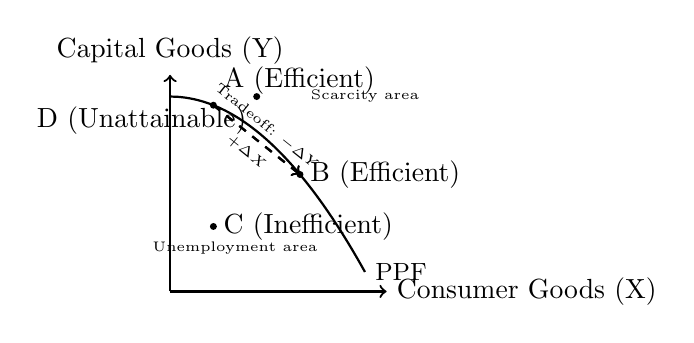
\begin{tikzpicture}[scale=0.55, thick]
    % Axes
    \draw[->] (0,0) -- (5,0) node[right] {Consumer Goods (X)};
    \draw[->] (0,0) -- (0,5) node[above] {Capital Goods (Y)};
    % PPF Curve
    \draw[domain=0:4.5, smooth] plot (\x, {4.5 - 0.2*\x*\x}) node[right] {\small PPF};
    % Points
    \filldraw (1,4.3) circle (1.5pt) node[above right] {A (Efficient)};
    \filldraw (3,2.7) circle (1.5pt) node[right] {B (Efficient)};
    \filldraw (2,4.5) circle (1.5pt) node[below left] {D (Unattainable)};
    \filldraw (1,1.5) circle (1.5pt) node[right] {C (Inefficient)};
    % Tradeoff arrow
    \draw[->, dashed] (1,4.3) -- node[above,sloped] {\tiny Tradeoff: $-\Delta Y$} (3,2.7);
    \draw[->, dashed] (1,4.3) -- node[below,sloped] {\tiny $+\Delta X$} (3,2.7);
    % Region labels
    \node at (4.5,4.5) {\tiny Scarcity area};
    \node at (1.5,1) {\tiny Unemployment area};
\end{tikzpicture}
\end{center}
\textit{Interpretation:} Scarcity forces choice between X and Y. Point D requires economic growth (shift outward). Point C shows idle resources. Movement A$\to$B incurs opportunity cost of lost capital goods.

\columnbreak

% --- ECONOMIC PROBLEMS ---
\section*{Basic Economic Problems}
\begin{enumerate}[leftmargin=*,nosep]
    \item \textbf{What to produce?} -- Choice of goods based on demand and resources.
    \item \textbf{How to produce?} -- Technique (labor/capital intensive), efficiency.
    \item \textbf{For whom to produce?} -- Distribution of income and output in society.
\end{enumerate}
\textbf{Source:} Rooted in \textbf{scarcity} of resources (land, labor, capital, entrepreneurship) versus unlimited human wants.

% --- CHOICE, TRADEOFF, OPPORTUNITY COST ---
\subsection*{Choice, Tradeoff, Opportunity Cost}
\begin{itemize}[leftmargin=*,nosep]
    \item \textbf{Choice:} Selecting one option over alternatives due to scarcity.
    \item \textbf{Tradeoff:} Sacrificing one goal to achieve another (all alternatives forgone).
    \item \textbf{Opportunity Cost:} The \textit{value} of the \textbf{next best alternative} forgone. Includes explicit + implicit costs.
    \[ OC = \text{Explicit Cost} + \text{Implicit Cost} \]
\end{itemize}

% --- ECONOMIC SYSTEMS ---
\subsection*{Economic Systems}
\begin{enumerate}[leftmargin=*,nosep]
    \item \textbf{Command Economy (Planned):}
    \begin{itemize}[nosep]
        \item Government controls production, prices, distribution.
        \item \textit{Ex: Former USSR, North Korea.}
        \item \textbf{Pro:} Low inequality. \textbf{Con:} Inefficiency, lacks innovation.
    \end{itemize}
    \item \textbf{Market Economy (Capitalism):}
    \begin{itemize}[nosep]
        \item Prices determined by supply/demand; private ownership.
        \item \textit{Ex: USA (19th century, laissez-faire).}
        \item \textbf{Pro:} Efficiency, innovation. \textbf{Con:} Inequality, market failures.
    \end{itemize}
    \item \textbf{Mixed Economy:}
    \begin{itemize}[nosep]
        \item Combines market mechanisms with government regulation and public services.
        \item \textit{Ex: Most modern economies (UK, France, India).}
        \item \textbf{Pro:} Balances efficiency and welfare. \textbf{Con:} Regulatory burden, taxation.
    \end{itemize}
\end{enumerate}

% --- MICRO vs MACRO ---
\subsection*{Microeconomics vs Macroeconomics}
\begin{itemize}[leftmargin=*,nosep]
    \item \textbf{Micro:} Study of \textit{individual} units -- households, firms, industries. Focus on demand/supply, prices, market structures. (\textit{Trees})
    \item \textbf{Macro:} Study of economy as a \textit{whole}. Focus on GDP, inflation, unemployment, monetary/fiscal policy. Aggregates. (\textit{Forest})
\end{itemize}
\textbf{Interdependence:} Macro outcomes arise from micro decisions; micro agents act within macro environment.

% --- CASE STUDIES ---
\subsection*{Case Studies}
\begin{enumerate}[leftmargin=*,nosep]
    \item \textbf{The Soviet Union (Command Economy):} Chronic shortages and surpluses occurred because central planners couldn’t set efficient prices. \textit{Concept:} Scarcity persisted despite planning; lack of tradeoff signals caused misallocation.
    \item \textbf{Covid-19 Vaccine Development (Choice \& Opportunity Cost):} Governments invested billions in vaccine research (Operation Warp Speed, US). The \textbf{opportunity cost} was forgone spending on other health programs or infrastructure. The \textbf{tradeoff} was speed vs. routine safety testing protocols.
\end{enumerate}

% --- EXAM QUESTIONS ---
\subsection*{Exam Practice}
\textbf{Q1:} Define opportunity cost. A farmer can grow 100 kg wheat or 200 kg rice on his land. What is the opportunity cost of growing 1 kg wheat?\\[0.1cm]
\textbf{Answer:} Opportunity cost is the next best alternative forgone. For 100 kg wheat, farmer sacrifices 200 kg rice. So, OC of 1 kg wheat = $\frac{200 \text{ kg rice}}{100 \text{ kg wheat}} = \mathbf{2 \text{ kg rice}}$.\\[0.2cm]

\textbf{Q2:} Why is scarcity considered a permanent economic problem even in rich countries?\\[0.1cm]
\textbf{Answer:} Scarcity arises from unlimited human wants vs. finite resources. Even wealthy nations cannot satisfy all desires (newer tech, better healthcare, leisure), forcing continuous choice and allocation decisions.


% --- DEFINITION ---
\section*{Definition}
\textbf{Demand:} The quantity of a good/service that consumers are \textbf{willing and able} to purchase at various prices over a given period, \textit{ceteris paribus}.

\textbf{Supply:} The quantity of a good/service that producers are \textbf{willing and able} to offer for sale at various prices over a given period, \textit{ceteris paribus}.

\textbf{Market Equilibrium:} The price where quantity demanded equals quantity supplied ($Q_d = Q_s$). No tendency for change.

% --- HOW TO REMIND ---
\subsection*{Memory Triggers}
\begin{itemize}[leftmargin=*,nosep]
    \item \textbf{Demand: ``D''ownward slope -- Price $\uparrow$, Quantity Demanded $\downarrow$} (Law of Demand).
    \item \textbf{Supply: ``S''kyward slope -- Price $\uparrow$, Quantity Supplied $\uparrow$} (Law of Supply).
    \item \textbf{Movement = Price change} (along curve). \textbf{Shift = Non-price factor} (whole curve moves).
    \item \textbf{Mnemonic for Demand Shifters -- ``PIRATES'':} \textbf{P}opulation, \textbf{I}ncome, \textbf{R}elated goods prices, \textbf{A}dvertising/Tastes, \textbf{T}axes, \textbf{E}xpectations, \textbf{S}eason.
\end{itemize}

% --- MATHEMATICAL TERM ---
\subsection*{Mathematical Representation}
\textbf{Demand Function:} $Q_d = a - bP$ \quad (Linear, inverse relationship)
\textbf{Supply Function:} $Q_s = c + dP$ \quad (Linear, direct relationship)
\textbf{Equilibrium Condition:}
\[
Q_d = Q_s \quad \Rightarrow \quad a - bP = c + dP
\]
\[
P^* = \frac{a-c}{b+d}, \qquad Q^* = a - b\left(\frac{a-c}{b+d}\right)
\]
Where $a, c$ = intercepts; $b, d$ = slopes (responsiveness to price).
\textbf{Excess Demand:} $Q_d > Q_s$ (shortage). \textbf{Excess Supply:} $Q_s > Q_d$ (surplus).

% --- GRAPH STUDY ---
\subsection*{Graph Study: Market Equilibrium}
\begin{center}
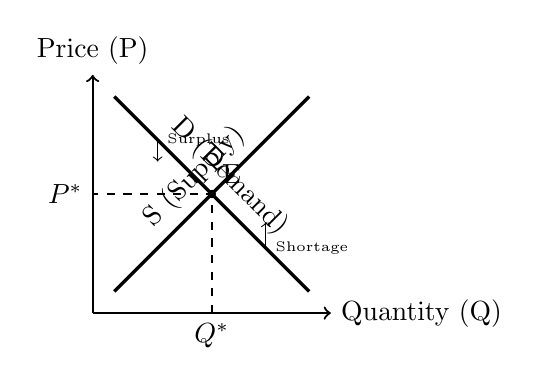
\begin{tikzpicture}[scale=0.55, thick]
    % Axes
    \draw[->] (0,0) -- (5.5,0) node[right] {Quantity (Q)};
    \draw[->] (0,0) -- (0,5.5) node[above] {Price (P)};
    % Demand curve
    \draw[very thick] (0.5,5) -- (5,0.5) node[midway, above, sloped] {D (Demand)};
    % Supply curve
    \draw[very thick] (0.5,0.5) -- (5,5) node[midway, above, sloped] {S (Supply)};
    % Equilibrium point
    \filldraw (2.75,2.75) circle (2pt) node[above right] {E};
    \draw[dashed] (2.75,0) node[below] {$Q^*$} -- (2.75,2.75) -- (0,2.75) node[left] {$P^*$};
    % Surplus region
    \draw[->, thin] (1.5,4) node[right] {\tiny Surplus} -- (1.5,3.5);
    % Shortage region
    \draw[->, thin] (4,1.5) node[right] {\tiny Shortage} -- (4,2.1);
\end{tikzpicture}
\end{center}
\textit{Interpretation:} At $P > P^*$, surplus drives price down. At $P < P^*$, shortage drives price up. Market forces push toward equilibrium automatically.

% --- MOVEMENTS vs SHIFTS ---
\subsection*{Movements Along vs. Shifts}
\begin{center}
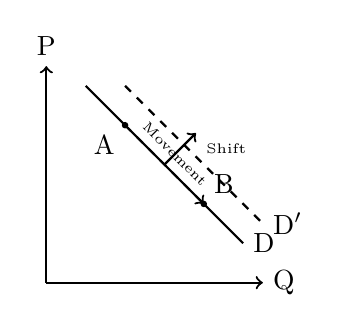
\begin{tikzpicture}[scale=0.5, thick]
    % Axes
    \draw[->] (0,0) -- (5.5,0) node[right] {Q};
    \draw[->] (0,0) -- (0,5.5) node[above] {P};
    % Demand curve
    \draw (1,5) -- (5,1) node[right] {D};
    % Movement along
    \filldraw (2,4) circle (1.5pt) node[below left] {A};
    \filldraw (4,2) circle (1.5pt) node[above right] {B};
    \draw[->, dashed] (2,4) -- (4,2) node[midway, above, sloped] {\tiny Movement};
    % Shift right
    \draw[dashed] (2,5) -- (5.5,1.5) node[right] {D$'$};
    \draw[->] (3,3) -- (3.8,3.8) node[below right] {\tiny Shift};
\end{tikzpicture}
\end{center}
\textbf{Movement:} Caused by change in own price (contraction/expansion).\\
\textbf{Shift:} Caused by non-price determinants (increase/decrease in demand/supply).

\columnbreak

% --- FACTORS INFLUENCING ---
\section*{Factors Influencing Demand \& Supply}

\subsection*{Demand Determinants (Shifters)}
\begin{enumerate}[leftmargin=*,nosep]
    \item \textbf{Income:} Normal goods (demand $\uparrow$ with income); Inferior goods (demand $\downarrow$).
    \item \textbf{Prices of Related Goods:} Substitutes (tea $\uparrow$ $\to$ coffee demand $\uparrow$); Complements (car $\uparrow$ $\to$ petrol demand $\downarrow$).
    \item \textbf{Tastes \& Preferences:} Trends, advertising, seasons.
    \item \textbf{Expectations:} Future price rise $\to$ current demand $\uparrow$.
    \item \textbf{Number of Buyers:} Population growth $\to$ demand $\uparrow$.
    \item \textbf{Government Policies:} Taxes, subsidies.
\end{enumerate}

\subsection*{Supply Determinants (Shifters)}
\begin{enumerate}[leftmargin=*,nosep]
    \item \textbf{Input/Cost of Production:} Raw material, labor cost $\uparrow$ $\to$ supply $\downarrow$.
    \item \textbf{Technology:} Improvement $\to$ supply $\uparrow$.
    \item \textbf{Prices of Related Goods in Production:} Substitutes in supply (wheat vs corn).
    \item \textbf{Expectations:} Future price $\uparrow$ $\to$ current supply $\downarrow$ (withhold).
    \item \textbf{Number of Sellers:} More firms $\to$ market supply $\uparrow$.
    \item \textbf{Natural Factors:} Weather, disasters (especially agriculture).
    \item \textbf{Government Policies:} Subsidies $\uparrow$ supply; taxes $\downarrow$ supply.
\end{enumerate}

% --- SCHEDULES ---
\subsection*{Demand \& Supply Schedules}
\textit{Individual Demand Schedule (Orange Market):}
\begin{center}
\begin{tabular}{|c|c|}
\hline
Price (\$/kg) & Qty Demanded (kg/week) \\
\hline
5 & 2 \\
4 & 4 \\
3 & 6 \\
2 & 8 \\
1 & 10 \\
\hline
\end{tabular}
\end{center}
\textit{Market Supply Schedule (Orange Market):}
\begin{center}
\begin{tabular}{|c|c|}
\hline
Price (\$/kg) & Qty Supplied (kg/week) \\
\hline
5 & 12 \\
4 & 10 \\
3 & 8 \\
2 & 6 \\
1 & 4 \\
\hline
\end{tabular}
\end{center}
\textbf{Market Demand/Supply:} Horizontal summation of all individual demand/supply curves at each price. $Q_{\text{market}} = \sum Q_{\text{individual}}$.

% --- LAW OF DEMAND ---
\subsection*{Law of Demand}
\textit{Ceteris paribus}, there is an \textbf{inverse relationship} between price and quantity demanded.
\begin{itemize}[leftmargin=*,nosep]
    \item \textbf{Reasons:} Income effect (purchasing power), Substitution effect (relatively cheaper alternatives).
    \item \textbf{Exceptions (Giffen/Veblen goods):} Price $\uparrow$ $\to$ demand $\uparrow$ (rare).
\end{itemize}

% --- EFFECTS OF SHIFTS ON EQUILIBRIUM ---
\subsection*{Shifts Effects on Equilibrium}
\begin{center}
\begin{tabular}{|c|c|c|c|}
\hline
\textbf{Change} & \textbf{D} & \textbf{S} & \textbf{P*, Q*} \\
\hline
D $\uparrow$ & Shift right & Constant & P $\uparrow$, Q $\uparrow$ \\
D $\downarrow$ & Shift left & Constant & P $\downarrow$, Q $\downarrow$ \\
S $\uparrow$ & Constant & Shift right & P $\downarrow$, Q $\uparrow$ \\
S $\downarrow$ & Constant & Shift left & P $\uparrow$, Q $\downarrow$ \\
\hline
\end{tabular}
\end{center}
\textbf{Simultaneous Shifts:} Effect on P and Q depends on relative magnitudes of shifts (draw graphs).

% --- SPECIAL CASES ---
\subsection*{Special Cases}
\begin{enumerate}[leftmargin=*,nosep]
    \item \textbf{Perfectly Inelastic Demand ($Q_d$ fixed):} Vertical demand curve (e.g., life-saving drug). Supply shift only changes price, quantity unchanged.
    \item \textbf{Perfectly Elastic Demand:} Horizontal demand curve (e.g., identical products in perfect competition). Any price above market $\to$ demand zero.
    \item \textbf{Price Floor (Minimum Price):} Set above equilibrium $\to$ persistent surplus (e.g., agricultural support price).
    \item \textbf{Price Ceiling (Maximum Price):} Set below equilibrium $\to$ persistent shortage (e.g., rent control).
    \item \textbf{Black Markets:} Emerge under binding price ceilings where goods sell at illegal higher prices.
\end{enumerate}

% --- CASE STUDIES ---
\subsection*{Case Studies}
\begin{enumerate}[leftmargin=*,nosep]
    \item \textbf{Housing Crisis \& Rent Control (New York, WWII):} Price ceiling on rents kept housing below market rate. Result: Persistent \textbf{shortage} of rental units, deterioration of buildings, black market sublets. \textit{Concept:} Binding price ceiling below equilibrium creates excess demand.
    \item \textbf{Global Semiconductor Shortage (2020--2022):} COVID disrupted supply chains ($S \downarrow$), while demand for electronics spiked with remote work ($D \uparrow$). Result: Prices rose sharply, auto industry stalled. \textit{Concept:} Simultaneous leftward supply shift and rightward demand shift $\to$ unambiguously higher price, ambiguous quantity effect (here Q fell due to dominant supply shock).
\end{enumerate}

% --- EXAM QUESTIONS ---
\subsection*{Exam Practice}
\textbf{Q1:} The demand and supply functions for a good are: $Q_d = 100 - 5P$ and $Q_s = 20 + 3P$. Find equilibrium price and quantity.\\[0.1cm]
\textbf{Answer:} Set $Q_d = Q_s$: $100 - 5P = 20 + 3P \Rightarrow 8P = 80 \Rightarrow \mathbf{P^* = 10}$. $Q^* = 100 - 5(10) = \mathbf{50}$ units.\\[0.2cm]

\textbf{Q2:} Distinguish between a ``movement along'' and a ``shift in'' the demand curve using an example.\\[0.1cm]
\textbf{Answer:} A movement along occurs when own price changes (e.g., price of apples falls from \$3 to \$2 $\to$ quantity demanded rises -- Law of Demand). A shift occurs when a non-price determinant changes (e.g., health study reveals apples reduce disease risk $\to$ demand curve shifts right, more bought at every price).\\[0.2cm]

\textbf{Q3:} Explain the effect of a government subsidy to wheat farmers on the equilibrium price and quantity of wheat. Illustrate.\\[0.1cm]
\textbf{Answer:} A subsidy reduces production costs, shifting the \textbf{supply curve rightward} ($S \to S'$). This creates surplus at original price, driving price \textbf{down} and equilibrium quantity \textbf{up}. Consumers benefit from lower prices; producers receive price + subsidy.
\end{multicols}
\end{document}
\newpage

% ============================================================================
% TOPIC 2: Demand and Supply
% ============================================================================
\documentclass[10pt,a4paper]{article}
\usepackage[margin=0.7in]{geometry}
\usepackage{multicol}
\usepackage{amsmath}
\usepackage{tikz}
\usepackage{enumitem}
\usepackage{titlesec}
\usepackage{booktabs}
\usepackage{fontspec}
\usepackage{xcolor}

% Compact formatting
\setlength{\columnsep}{0.7cm}
\setlength{\parindent}{0pt}
\setlength{\parskip}{0.12cm}
\titlespacing{\section}{0pt}{0.4cm}{0.15cm}
\titlespacing{\subsection}{0pt}{0.25cm}{0.08cm}
\titlespacing{\subsubsection}{0pt}{0.2cm}{0.05cm}

% Custom section style
\titleformat{\section}{\large\bfseries}{}{0em}{}
\titleformat{\subsection}{\normalsize\bfseries}{}{0em}{}
\titleformat{\subsubsection}{\normalsize\bfseries\itshape}{}{0em}{}

\begin{document}

\begin{center}
{\LARGE \textbf{Demand, Supply \& Market Equilibrium}}\\[0.15cm]
{\normalsize \textit{Topic 2: The Price Mechanism and Resource Allocation}}\\[0.15cm]
\hrule
\end{center}
\vspace{-0.3cm}

\begin{multicols}{2}
\footnotesize

% ============================================================================
% PART 1: DEFINITIONS AND FOUNDATIONS
% ============================================================================
\section*{1. Core Definitions}

\subsection*{Demand (Detailed)}
\textbf{Demand} is not merely desire; it is \textbf{effective demand} -- the quantity of a good or service that consumers are both \textit{willing} and \textit{financially able} to purchase at each possible price during a specific time period, holding all other factors constant (\textit{ceteris paribus}).

\textbf{Key Elements:}
\begin{itemize}[leftmargin=*,nosep]
    \item \textbf{Willingness:} Derived from utility/preference.
    \item \textbf{Ability:} Backed by purchasing power (income).
    \item \textbf{Time Dimension:} Flow concept (per day/week/year).
    \item \textbf{Price Range:} A schedule, not a single quantity.
\end{itemize}

\textbf{Individual vs. Market Demand:} Market demand is the \textbf{horizontal summation} of all individual demand curves. If consumer A demands 3 units at \$5 and consumer B demands 4 units at \$5, market demand at \$5 is $3+4=7$ units.

\subsection*{Supply (Detailed)}
\textbf{Supply} represents the quantity of a good or service that producers are willing and able to bring to market at each possible price over a given period, \textit{ceteris paribus}.

\textbf{Key Elements:}
\begin{itemize}[leftmargin=*,nosep]
    \item \textbf{Willingness:} Profit motive; price must cover marginal cost.
    \item \textbf{Ability:} Production capacity, technology, resource access.
    \item \textbf{Time Dimension:} Supply elasticity varies with time horizon.
\end{itemize}

% ============================================================================
% PART 2: MEMORY TRIGGERS AND CONCEPTUAL ANCHORS
% ============================================================================
\section*{2. How to Remember (Conceptual Anchors)}

\begin{enumerate}[leftmargin=*,nosep]
    \item \textbf{Demand = Consumer Story:} ``Price high? I buy less.'' (Downward slope). Imagine yourself at a store -- sale prices entice, high prices repel.
    \item \textbf{Supply = Producer Story:} ``Price high? I produce more!'' (Upward slope). Higher price means higher profit margin; firms expand output.
    \item \textbf{Movement vs. Shift -- The ``P'' Test:}
    \begin{itemize}[nosep]
        \item If only \textbf{P} (own price) changes $\to$ \textbf{Movement} along the curve.
        \item If any other factor changes $\to$ \textbf{Shift} of the entire curve.
    \end{itemize}
    \item \textbf{Demand Shifters -- ``PIRATES-CO''}: \textbf{P}opulation, \textbf{I}ncome, \textbf{R}elated goods, \textbf{A}dvertising/Taste, \textbf{T}axes, \textbf{E}xpectations, \textbf{S}eason -- \textbf{C}redit, \textbf{O}ther factors.
    \item \textbf{Supply Shifters -- ``TIC-NES''}: \textbf{T}echnology, \textbf{I}nput costs, \textbf{C}ompeting goods (in production) -- \textbf{N}atural factors, \textbf{E}xpectations, \textbf{S}ellers (number of).
    \item \textbf{Equilibrium = Balance Point}: Imagine a see-saw; the market price is the pivot where the weight of buyers (demand) exactly balances the weight of sellers (supply).
\end{enumerate}

% ============================================================================
% PART 3: MATHEMATICAL FRAMEWORK
% ============================================================================
\section*{3. Mathematical Formulation and Analysis}

\subsection*{Linear Demand Function}
\[
Q_d = a - bP
\]
Where: $a$ = quantity demanded when $P=0$ (intercept), $b$ = slope coefficient (rate at which $Q_d$ changes with $P$). Note: $b > 0$, indicating inverse relationship. \textbf{Inverse Demand:} $P = \frac{a}{b} - \frac{1}{b}Q_d$ (useful for graphing with $P$ on vertical axis).

\subsection*{Linear Supply Function}
\[
Q_s = c + dP
\]
Where: $c$ = quantity supplied when $P=0$ (often negative, as firms need a minimum price to produce), $d$ = slope coefficient ($d > 0$, direct relationship). \textbf{Inverse Supply:} $P = \frac{-c}{d} + \frac{1}{d}Q_s$.

\subsection*{Equilibrium Solution}
At equilibrium, $\mathbf{Q_d = Q_s}$:
\begin{align*}
a - bP &= c + dP \\
a - c &= (b + d)P \\
P^* &= \frac{a - c}{b + d}
\end{align*}
Substituting $P^*$ into either function yields $Q^*$.

\subsection*{Numerical Example}
Given: $Q_d = 80 - 4P$ and $Q_s = -10 + 6P$.
\[
80 - 4P = -10 + 6P \;\Rightarrow\; 90 = 10P \;\Rightarrow\; \mathbf{P^* = 9}
\]
\[
Q^* = 80 - 4(9) = 44 \quad \text{(or } -10 + 6(9) = 44\text{)}
\]

\subsection*{Consumer and Producer Surplus (Advanced)}
\begin{itemize}[leftmargin=*,nosep]
    \item \textbf{Consumer Surplus (CS):} Area below demand curve, above price, up to $Q^*$. $CS = \frac{1}{2} \times Q^* \times (\text{Choke Price} - P^*)$, where choke price = $a/b$.
    \item \textbf{Producer Surplus (PS):} Area above supply curve, below price, up to $Q^*$. $PS = \frac{1}{2} \times Q^* \times (P^* - \text{Min Supply Price})$.
    \item \textbf{Total Welfare:} $CS + PS$; maximized at free-market equilibrium.
\end{itemize}

% ============================================================================
% PART 4: GRAPHICAL ANALYSIS
% ============================================================================
\section*{4. Graphical Analysis}

\subsection*{Basic Market Equilibrium}
\begin{center}
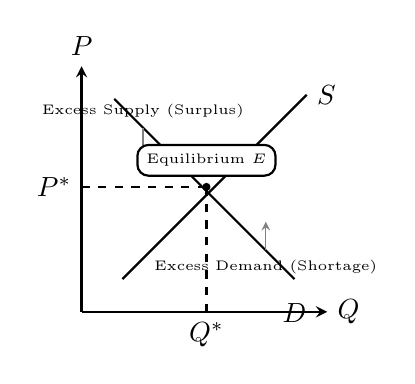
\begin{tikzpicture}[scale=0.52, thick, >=stealth]
    \draw[->] (0,0) -- (6,0) node[right] {$Q$};
    \draw[->] (0,0) -- (0,6) node[above] {$P$};
    \draw[thick] (0.8,5.2) -- (5.2,0.8) node[below=5pt] {$D$};
    \draw[thick] (1,0.8) -- (5.5,5.3) node[right] {$S$};
    \filldraw (3.05,3.05) circle (2pt);
    \draw[dashed] (3.05,0) node[below] {$Q^*$} -- (3.05,3.05);
    \draw[dashed] (0,3.05) node[left] {$P^*$} -- (3.05,3.05);
    % Surplus zone (P > P*)
    \draw[->, thin, gray] (1.5,4.5) node[above, black] {\tiny Excess Supply (Surplus)} -- (1.5,3.8);
    \draw[->, thin, gray] (4.5,1.5) node[below, black] {\tiny Excess Demand (Shortage)} -- (4.5,2.2);
    \node[draw, fill=white, rounded corners] at (3.05,3.7) {\tiny Equilibrium $E$};
\end{tikzpicture}
\end{center}

\subsection*{Panel A: Shift in Demand (Increase)}
\begin{center}
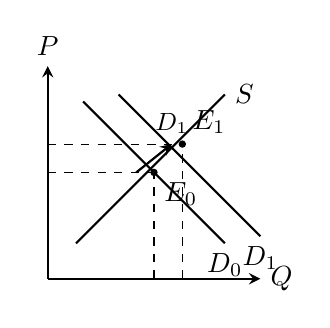
\begin{tikzpicture}[scale=0.45, thick, >=stealth]
    \draw[->] (0,0) -- (6,0) node[right] {$Q$};
    \draw[->] (0,0) -- (0,6) node[above] {$P$};
    \draw (1,5) -- (5,1) node[below] {$D_0$};
    \draw[thick, ->] (2.5,3) -- (3.5,3.8) node[above] {\small $D_1$};
    \draw (2,5.2) -- (6,1.2) node[below] {$D_1$};
    \draw (0.8,1) -- (5,5.2) node[right] {$S$};
    \filldraw (3,3) circle (2pt) node[below right] {$E_0$};
    \filldraw (3.8,3.8) circle (2pt) node[above right] {$E_1$};
    \draw[dashed, thin] (3,0) -- (3,3); \draw[dashed, thin] (3.8,0) -- (3.8,3.8);
    \draw[dashed, thin] (0,3) -- (3,3); \draw[dashed, thin] (0,3.8) -- (3.8,3.8);
\end{tikzpicture}
\end{center}
\textbf{Result:} $P^* \uparrow$, $Q^* \uparrow$. Caused by: income rise, preference surge, price of substitute rises, etc.

\subsection*{Panel B: Shift in Supply (Decrease)}
\begin{center}
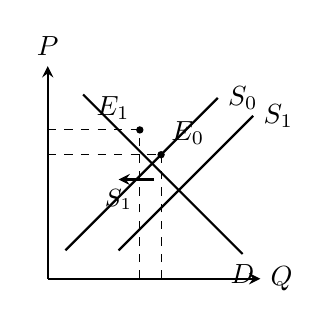
\begin{tikzpicture}[scale=0.45, thick, >=stealth]
    \draw[->] (0,0) -- (6,0) node[right] {$Q$};
    \draw[->] (0,0) -- (0,6) node[above] {$P$};
    \draw (1,5.2) -- (5.5,0.7) node[below] {$D$};
    \draw (0.5,0.8) -- (4.8,5.1) node[right] {$S_0$};
    \draw[thick, ->] (3,2.8) -- (2,2.8) node[below] {\small $S_1$};
    \draw (2,0.8) -- (5.8,4.6) node[right] {$S_1$};
    \filldraw (3.2,3.5) circle (2pt) node[above right] {$E_0$};
    \filldraw (2.6,4.2) circle (2pt) node[above left] {$E_1$};
    \draw[dashed, thin] (3.2,0) -- (3.2,3.5);
    \draw[dashed, thin] (2.6,0) -- (2.6,4.2);
    \draw[dashed, thin] (0,3.5) -- (3.2,3.5);
    \draw[dashed, thin] (0,4.2) -- (2.6,4.2);
\end{tikzpicture}
\end{center}
\textbf{Result:} $P^* \uparrow$, $Q^* \downarrow$. Caused by: input cost rise, natural disaster, tax increase, fewer sellers.

\columnbreak

% ============================================================================
% PART 5: DETERMINANTS (DETAILED EXPLANATIONS)
% ============================================================================
\section*{5. Factors Influencing Demand \& Supply (In-Depth)}

\subsection*{Demand Determinants (Shifters)}
\begin{enumerate}[leftmargin=*,nosep]
    \item \textbf{Income:}
    \begin{itemize}[nosep]
        \item \textbf{Normal Goods:} Income $\uparrow \to$ Demand $\uparrow$ (e.g., branded clothing, restaurant meals). Demand curve shifts \textbf{right}.
        \item \textbf{Inferior Goods:} Income $\uparrow \to$ Demand $\downarrow$ (e.g., instant noodles, public bus transport). Demand curve shifts \textbf{left}.
    \end{itemize}
    \item \textbf{Prices of Related Goods:}
    \begin{itemize}[nosep]
        \item \textbf{Substitutes:} Goods that satisfy similar wants (tea \& coffee). Price of coffee $\uparrow$ $\to$ demand for tea $\uparrow$ (shift right).
        \item \textbf{Complements:} Goods used together (car \& petrol, printer \& ink). Price of car $\uparrow$ $\to$ demand for petrol $\downarrow$ (shift left).
        \item \textbf{Cross-Price Elasticity:} $E_{xy} = \frac{\%\Delta Q_x}{\%\Delta P_y}$. Positive for substitutes, negative for complements.
    \end{itemize}
    \item \textbf{Tastes, Preferences \& Social Trends:} Advertising, celebrity endorsements, cultural shifts, health consciousness (e.g., demand for organic food rising).
    \item \textbf{Consumer Expectations:}
    \begin{itemize}[nosep]
        \item Future price rise expected $\to$ current demand $\uparrow$ (buy now before it's expensive).
        \item Future income rise expected $\to$ current demand $\uparrow$ (spend confidently today).
    \end{itemize}
    \item \textbf{Demographics (Population):} Larger population $\to$ more buyers $\to$ market demand shifts right. Aging population changes composition of demand (more healthcare, less baby products).
    \item \textbf{Government Policies:} Subsidies to consumers (e.g., electric vehicle rebate) shift demand right; taxes on goods (e.g., sugar tax) shift demand left.
    \item \textbf{Seasonal/Climatic Factors:} Demand for ice cream rises in summer, woolen clothes in winter.
    \item \textbf{Availability of Credit:} Easy loans/EMIs $\to$ demand for durable goods (cars, homes) rises.
\end{enumerate}

\subsection*{Supply Determinants (Shifters)}
\begin{enumerate}[leftmargin=*,nosep]
    \item \textbf{Input Prices (Cost of Production):} Wages $\uparrow$, raw material $\uparrow$, energy cost $\uparrow$ $\to$ production cost $\uparrow$ $\to$ supply shifts \textbf{left}. Vice versa.
    \item \textbf{Technology:} Technological progress lowers cost per unit $\to$ supply shifts \textbf{right}. (e.g., automation in manufacturing, AI-driven logistics).
    \item \textbf{Prices of Related Goods in Production:}
    \begin{itemize}[nosep]
        \item \textbf{Substitutes in Production:} A farmer can grow wheat or corn on the same land. Corn price $\uparrow$ $\to$ farmer shifts land to corn $\to$ supply of wheat $\downarrow$ (shift left).
        \item \textbf{Joint Products:} Beef and leather are joint products. Beef demand $\uparrow$ $\to$ leather supply $\uparrow$ (shift right).
    \end{itemize}
    \item \textbf{Producer Expectations:} If firms expect higher future prices, they may withhold current supply (shift left) to sell later at a profit.
    \item \textbf{Number of Sellers (Market Structure):} More firms entering the industry $\to$ market supply shifts \textbf{right}. Exit $\to$ shifts left.
    \item \textbf{Natural/Social Factors:} Weather (drought, flood), pandemics, strikes, war disrupt production $\to$ supply shifts left.
    \item \textbf{Government Policies:}
    \begin{itemize}[nosep]
        \item \textbf{Subsidies:} Reduce effective cost $\to$ supply shifts right.
        \item \textbf{Taxes (Indirect):} Increase cost $\to$ supply shifts left.
        \item \textbf{Regulations:} Environmental/safety compliance costs $\to$ supply shifts left.
    \end{itemize}
\end{enumerate}

% ============================================================================
% PART 6: MARKET EQUILIBRIUM MECHANISM
% ============================================================================
\section*{6. Price Theory: The Market Mechanism}

\subsection*{The Invisible Hand (Adam Smith)}
Prices act as \textbf{signals} in a market economy. When a shortage exists ($Q_d > Q_s$), buyers bid prices up; the higher price incentivizes producers to supply more and discourages some consumption, moving the market toward equilibrium. Conversely, a surplus ($Q_s > Q_d$) leads firms to cut prices, clearing the market. No central planner is needed -- the \textbf{price mechanism} coordinates millions of independent decisions.

\subsection*{Comparative Statics: Effects of Shifts}
\begin{center}
\begin{tabular}{@{}p{1.8cm}p{1.5cm}p{1.2cm}p{1.2cm}@{}}
\toprule
\textbf{Scenario} & \textbf{Shift} & \textbf{$\Delta P^*$} & \textbf{$\Delta Q^*$} \\
\midrule
$D \uparrow$, $S$ constant & $D$ right & $\uparrow$ & $\uparrow$ \\
$D \downarrow$, $S$ constant & $D$ left & $\downarrow$ & $\downarrow$ \\
$S \uparrow$, $D$ constant & $S$ right & $\downarrow$ & $\uparrow$ \\
$S \downarrow$, $D$ constant & $S$ left & $\uparrow$ & $\downarrow$ \\
\addlinespace
$D \uparrow$, $S \uparrow$ (equal) & Both right & \textbf{Same} & $\uparrow$ \\
$D \uparrow$, $S \downarrow$ & $D$ right, $S$ left & $\uparrow$ & \textbf{Ambiguous} \\
$D \downarrow$, $S \uparrow$ & $D$ left, $S$ right & $\downarrow$ & \textbf{Ambiguous} \\
$D \downarrow$, $S \downarrow$ & Both left & \textbf{Ambiguous} & $\downarrow$ \\
\bottomrule
\end{tabular}
\end{center}

\subsection*{Special Cases in Detail}
\begin{enumerate}[leftmargin=*,nosep]
    \item \textbf{Perfectly Inelastic Demand (Vertical $D$):} $E_d = 0$. Quantity demanded fixed regardless of price (e.g., life-saving insulin). Any shift in supply changes only price; quantity remains unchanged. A supply reduction severely raises price without reducing consumption -- a policy concern.
    \item \textbf{Perfectly Elastic Demand (Horizontal $D$):} $E_d = \infty$. Consumers will buy any quantity at exactly one price, but nothing above it (e.g., agricultural commodities in a perfectly competitive global market). A single producer cannot raise price without losing all customers.
    \item \textbf{Government Price Controls:}
    \begin{itemize}[nosep]
        \item \textbf{Price Ceiling} (below $P^*$): Creates persistent \textbf{shortage}. Legal maximum price (e.g., rent control). Quantity supplied falls, quantity demanded rises $\to$ excess demand.
        \item \textbf{Price Floor} (above $P^*$): Creates persistent \textbf{surplus}. Legal minimum price (e.g., agricultural price supports, minimum wage). Quantity supplied exceeds quantity demanded $\to$ excess supply.
    \end{itemize}
    \item \textbf{Veblen Goods (Conspicuous Consumption):} As price rises, snob appeal increases $\to$ demand rises. An \textbf{exception} to the Law of Demand (luxury brands, diamonds).
    \item \textbf{Giffen Goods:} Staple inferior good (e.g., bread in 19th century Ireland). Price rise soaks up so much income that consumers buy more of the staple and less of superior goods (potatoes vs. meat). Extremely rare.
\end{enumerate}

% ============================================================================
% PART 7: EXTENSIVE CASE STUDIES
% ============================================================================
\section*{7. Comprehensive Case Studies}

\subsection*{Case Study 1: The Global Semiconductor Chip Crisis (2020--2023)}

\textbf{Background:} Semiconductors are essential inputs for automobiles, smartphones, medical devices, and virtually all modern electronics. The industry is concentrated in Taiwan (TSMC), South Korea (Samsung), and a few other players.

\textbf{Events (Chronological Analysis):}

\textit{Early 2020 -- Demand Shock:} COVID-19 pandemic triggers global lockdowns. Automakers, anticipating a prolonged recession, \textbf{cancel semiconductor orders}. Simultaneously, remote work and online learning surge, causing a massive spike in demand for laptops, tablets, gaming consoles, and cloud computing hardware. \textbf{Demand for chips shifts sharply right} in consumer electronics segment.

\textit{Mid 2020--2021 -- Supply Shock:} Chip fabrication plants (fabs) face COVID-related shutdowns, worker shortages, and logistics bottlenecks. Key raw material (silicon wafers) supply tightens. A major fire at Renesas plant (Japan, March 2021) and drought in Taiwan (water-intensive chip production) further constrain output. \textbf{Supply curve shifts left dramatically.}

\textit{Late 2021--2022 -- Cascading Effects:} Automakers, having cancelled orders, find themselves at the back of the queue when they try to re-order. Chip foundries are running at full capacity fulfilling tech sector contracts. The auto industry, which uses less advanced chips, cannot get supply. \textbf{A double shock:} $D_{\text{overall}}$ right, $S_{\text{overall}}$ left.

\textbf{Economic Analysis Using Demand-Supply Framework:}

\begin{center}
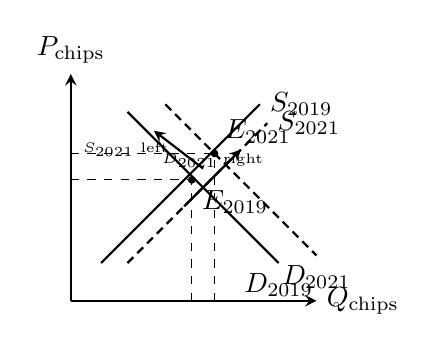
\begin{tikzpicture}[scale=0.48, thick, >=stealth]
    \draw[->] (0,0) -- (6.5,0) node[right] {$Q_{\text{chips}}$};
    \draw[->] (0,0) -- (0,6) node[above] {$P_{\text{chips}}$};
    % Original curves
    \draw (1.5,5) -- (5.5,1) node[below] {$D_{2019}$};
    \draw (0.8,1) -- (5,5.2) node[right] {$S_{2019}$};
    \filldraw (3.2,3.2) circle (2pt) node[below right] {$E_{2019}$};
    % New curves
    \draw[->, thick] (3,2.5) -- (4.5,4) node[midway, above] {\tiny $D_{2021}$ right};
    \draw[thick, densely dashed] (2.5,5.2) -- (6.5,1.2) node[below] {$D_{2021}$};
    \draw[->, thick] (3.5,3.5) -- (2.2,4.5) node[midway, left] {\tiny $S_{2021}$ left};
    \draw[thick, densely dashed] (1.5,1) -- (5.2,4.7) node[right] {$S_{2021}$};
    \filldraw (3.8,3.9) circle (2pt) node[above right] {$E_{2021}$};
    \draw[dashed, thin] (0,3.2) -- (3.2,3.2); \draw[dashed, thin] (0,3.9) -- (3.8,3.9);
    \draw[dashed, thin] (3.2,0) -- (3.2,3.2); \draw[dashed, thin] (3.8,0) -- (3.8,3.9);
\end{tikzpicture}
\end{center}

\textbf{Outcome:}
\begin{itemize}[leftmargin=*,nosep]
    \item \textbf{Price} of semiconductors rose dramatically (spot prices for some chips increased 300--500\%).
    \item \textbf{Quantity} effect was ambiguous in theory, but in practice, severe supply constraints meant overall unit shipments fell slightly despite skyrocketing demand.
    \item \textbf{Automotive Knock-on Effects:} Car production dropped; new car inventory collapsed; used car prices in the US spiked over 40\% year-on-year (a market for a \textit{complement} good affected). Global auto industry lost an estimated \$210 billion in revenue in 2021.
    \item \textbf{Policy Response:} US CHIPS Act (\$52 billion subsidies) aimed to shift \textbf{supply right} long-term by incentivizing domestic fabrication.
\end{itemize}

\textbf{Economic Lessons:}
\begin{enumerate}[leftmargin=*,nosep]
    \item Simultaneous demand increase and supply decrease unambiguously raises price.
    \item Concentrated supply chains create systemic vulnerability.
    \item Government subsidies (supply-side policy) can be justified to address strategic shortages.
    \item Markets are interconnected; a shortage in one input (chips) cascades to final goods (cars, electronics).
\end{enumerate}

\subsection*{Case Study 2: Rent Control in New York City -- A Persistent Price Ceiling}

\textbf{Background:} New York City implemented rent control during World War II (1943 Emergency Price Control Act) to prevent profiteering during a housing shortage. While most US cities abandoned controls, NYC retained \textbf{rent stabilization} covering approximately 1 million apartments today.

\textbf{Mechanism:} The government sets a maximum price (ceiling) below the market equilibrium. Let free-market rent be $P^* = \$2,500/\text{month}$, and rental units available = $Q^* = 500,000$. The city imposes a ceiling at $P_c = \$1,500/\text{month}$.

\textbf{Analyzing the Market:}

At $P_c = \$1,500$:
\begin{itemize}[leftmargin=*,nosep]
    \item \textbf{Quantity Supplied ($Q_s$):} At the artificially low price, landlords have reduced incentive to maintain existing units, construct new rental buildings, or even keep properties in the rental market (conversion to condos/co-ops). $Q_s$ falls to, say, $350,000$ units.
    \item \textbf{Quantity Demanded ($Q_d$):} The lower price makes renting more attractive relative to buying, and more households form (roommates splitting, etc.). $Q_d$ rises to $650,000$ units.
    \item \textbf{Shortage:} Persistent excess demand of $650,000 - 350,000 = 300,000$ units.
\end{itemize}

\begin{center}
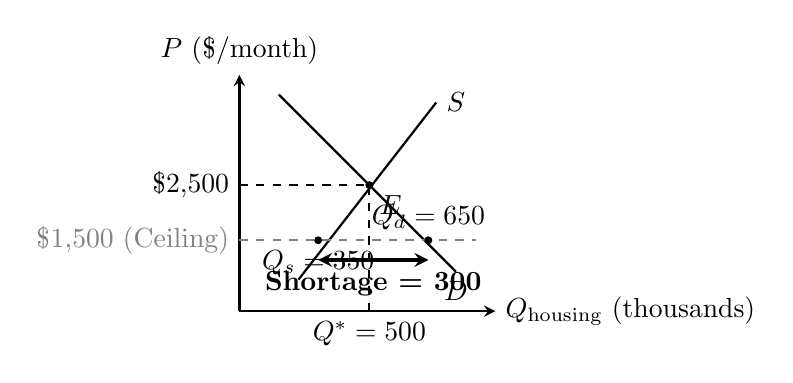
\begin{tikzpicture}[scale=0.5, thick, >=stealth]
    \draw[->] (0,0) -- (6.5,0) node[right] {$Q_{\text{housing}}$ (thousands)};
    \draw[->] (0,0) -- (0,6) node[above] {$P$ (\$/month)};
    \draw (1,5.5) -- (5.5,1) node[below] {$D$};
    \draw (1.5,0.8) -- (5,5.3) node[right] {$S$};
    \filldraw (3.3,3.2) circle (2pt) node[below right] {$E$};
    \draw[dashed, gray, thick] (0,1.8) node[left] {\$1,500 (Ceiling)} -- (6,1.8);
    \filldraw (2,1.8) circle (2pt) node[below] {$Q_s=350$};
    \filldraw (4.8,1.8) circle (2pt) node[above] {$Q_d=650$};
    \draw[<->, very thick] (2,1.3) -- (4.8,1.3) node[midway, below] {\textbf{Shortage = 300}};
    \draw[dashed] (3.3,0) node[below] {$Q^*=500$} -- (3.3,3.2);
    \draw[dashed] (0,3.2) node[left] {\$2,500} -- (3.3,3.2);
\end{tikzpicture}
\end{center}

\textbf{Observed Consequences (Documented by Economists):}

\begin{enumerate}[leftmargin=*,nosep]
    \item \textbf{Misallocation / ``Lock-in'' Effect:} Tenants in rent-controlled units stay for decades, even when the apartment no longer suits their needs (empty nesters in large three-bedrooms), because moving means losing the subsidy. Young families needing space cannot find it. This is \textbf{inefficient allocation} of a scarce resource.
    \item \textbf{Reduced Supply / Deterioration:} Landlords, receiving below-market returns, minimize maintenance (``deferred maintenance''). Buildings deteriorate. Some landlords abandon properties (1960s--70s NYC saw widespread abandonment and arson for insurance). New construction of rental units becomes unprofitable; developers build condos instead.
    \item \textbf{Black Market / Key Money:} Shortage creates illegal side payments. A prospective tenant might pay thousands of dollars ``under the table'' (``key money'') to a departing tenant or broker to secure a rent-controlled lease. The effective price paid (legal rent + key money) approximates the free-market price.
    \item \textbf{Discrimination:} With excess demand, landlords can be highly selective, leading to discrimination based on race, family status, or profession -- because many people compete for each vacancy.
    \item \textbf{Creation of a Dual Market:} A tier emerges: lucky incumbents paying far below market rate, and newcomers paying exorbitant free-market prices for the few available non-controlled units, leading to increased \textbf{inequality}.
    \item \textbf{Economist Consensus:} Surveys show over 90\% of economists agree rent control reduces the quantity and quality of available housing over time. Assar Lindbeck, a prominent economist, famously stated, ``In many cases, rent control appears to be the most efficient technique presently known to destroy a city -- except for bombing.''
\end{enumerate}

\textbf{Economic Lesson:} A binding price ceiling, however well-intentioned, creates a permanent shortage, promotes black markets, reduces quality, and generates deadweight welfare loss. The intended beneficiaries (low-income renters) may suffer from reduced availability and building decay.

% ============================================================================
% PART 8: EXAM QUESTIONS WITH DETAILED ANSWERS
% ============================================================================
\section*{8. Exam Practice Questions \& Model Answers}

\subsection*{Question 1: Analytical}
\textbf{The demand for good X is given by $Q_d = 1200 - 15P$ and supply is $Q_s = 200 + 10P$. The government imposes a per-unit tax of \$5 on producers.}
\textbf{(a) Find pre-tax equilibrium. (b) Find the new supply equation. (c) Calculate post-tax equilibrium price and quantity. (d) Determine tax incidence on consumers and producers. (e) Calculate deadweight loss.}

\vspace{0.1cm}
\textbf{Solution:}
\vspace{0.05cm}
\textbf{(a)} $1200 - 15P = 200 + 10P \Rightarrow 1000 = 25P \Rightarrow \mathbf{P_0^* = 40}$. $Q_0^* = 1200 - 15(40) = \mathbf{600}$.
\vspace{0.05cm}
\textbf{(b)} A \$5 tax on producers means they receive $(P - 5)$ for each unit. Supply function in terms of price received: $Q_s = 200 + 10(P_{\text{received}}) = 200 + 10(P - 5) = 200 + 10P - 50 = \mathbf{150 + 10P}$. New supply: $\mathbf{Q_{s,\text{new}} = 150 + 10P}$.
\vspace{0.05cm}
\textbf{(c)} New equilibrium: $1200 - 15P = 150 + 10P \Rightarrow 1050 = 25P \Rightarrow \mathbf{P_{\text{buyer}} = 42}$. $Q^* = 1200 - 15(42) = \mathbf{570}$. Price received by sellers: $P_{\text{seller}} = 42 - 5 = \mathbf{37}$.
\vspace{0.05cm}
\textbf{(d)} Tax incidence: Consumer pays \$42 (up from \$40, burden = \$2/unit). Producer receives \$37 (down from \$40, burden = \$3/unit). \textbf{Consumer burden: \$2; Producer burden: \$3.} Producers bear more because supply is relatively less elastic ($d=10$) compared to demand ($b=15$). Tax falls more heavily on the less elastic side.
\vspace{0.05cm}
\textbf{(e)} Deadweight loss = $\frac{1}{2} \times \text{Tax} \times \text{Change in Q} = \frac{1}{2} \times 5 \times (600 - 570) = 0.5 \times 5 \times 30 = \mathbf{\$75}$.

\vspace{0.2cm}

\subsection*{Question 2: Conceptual/Discussion}
\textbf{Using the demand-supply framework, explain the likely market effects of a government decision to provide free university education, funded by a tax on high-income earners. Discuss both the education market and potential unintended consequences.}

\vspace{0.1cm}
\textbf{Model Answer:}
Providing free university education is effectively a \textbf{zero price} imposed on students (a price ceiling at \$0) combined with a \textbf{subsidy} to institutions from tax revenue.

\textbf{In the Market for University Seats:}
\begin{itemize}[leftmargin=*,nosep]
    \item \textbf{Demand Side:} Personal cost to attend drops to zero (tuition = 0; though opportunity cost remains). Quantity demanded surges -- many students who would not have attended due to cost now enroll. Demand curve shifts right (or, if modeled as price change, a massive movement down the demand curve).
    \item \textbf{Supply Side:} The government must fund seats through tax revenue, shifting the effective supply curve right if funding is sufficient. However, quantity supplied depends on fiscal capacity. If funding per seat is below true cost, quality may erode.
    \item \textbf{Likely Outcome:} Excess demand (more applicants than funded seats) results in \textbf{non-price rationing} -- admission tests, GPA cutoffs become more competitive. This favors students with better prior schooling (often from higher socioeconomic backgrounds), potentially regressive despite the policy's progressive intent.
\end{itemize}
\textbf{Unintended Consequences:}
\begin{itemize}[leftmargin=*,nosep]
    \item \textbf{Labor Market:} A surge in graduates may depress the wage premium for a degree if demand for skilled labor doesn't keep pace (credential inflation).
    \item \textbf{Opportunity Cost Signal:} Zero tuition removes the price signal that guides students toward fields with high labor demand. Students may choose courses of personal interest over marketable skills, leading to eventual skills mismatch.
    \item \textbf{Tax Burden:} The increased tax on high-income earners may reduce their labor supply, savings, or investment (shift in supply of capital), creating a deadweight loss in other markets.
\end{itemize}
The final welfare effect is ambiguous and depends on the social return to education versus the efficiency cost of taxation.

\vspace{0.2cm}

\subsection*{Question 3: Short Numerical}
\textbf{In the market for coffee, $Q_d = 500 - 2P$ and $Q_s = -100 + 4P$. A technological breakthrough in coffee roasting reduces production cost, shifting supply to $Q_s = 0 + 4P$. Compare the old and new equilibria. Illustrate consumer gain.}

\vspace{0.1cm}
\textbf{Solution:}
\textit{Original:} $500 - 2P = -100 + 4P \Rightarrow 600 = 6P \Rightarrow P = 100, Q = 300$.
\textit{New:} $500 - 2P = 0 + 4P \Rightarrow 500 = 6P \Rightarrow P = 83.33, Q = 333.33$.
\textit{Change:} Price falls by \$16.67; quantity rises by 33.33 units. Consumer surplus increases (area between old and new price, bounded by demand curve). Lower prices benefit all coffee drinkers; producers may earn more total revenue if demand is elastic (here $E_d$ at new point = $|-2 \times 83.33/333.33| \approx 0.5$, inelastic, so TR might fall slightly, but increased volume may raise profit due to lower cost).

\end{multicols}

% ============================================================================
% SINGLE COLUMN SUMMARY TABLE (END OF DOCUMENT)
% ============================================================================
\vspace{0.3cm}
\begin{center}
\fbox{\begin{minipage}{0.9\textwidth}
\footnotesize
\textbf{Summary Table: Cheat Sheet for Exams}
\begin{center}
\begin{tabular}{@{}p{3cm}p{3.5cm}p{3.5cm}@{}}
\toprule
\textbf{Concept} & \textbf{Definition} & \textbf{Key Formula/Effect} \\
\midrule
Law of Demand & Price $\uparrow \to Q_d \downarrow$ & $\frac{\Delta Q_d}{\Delta P} < 0$ \\
Law of Supply & Price $\uparrow \to Q_s \uparrow$ & $\frac{\Delta Q_s}{\Delta P} > 0$ \\
Equilibrium & $Q_d = Q_s$ & $P^* = \frac{a-c}{b+d}$ \\
Movement vs Shift & \textbf{Movement:} Own price change. \textbf{Shift:} Non-price factor change. & Point on same curve vs. new curve. \\
Excess Demand & $Q_d > Q_s$ at given price & Shortage, upward pressure on P \\
Excess Supply & $Q_s > Q_d$ at given price & Surplus, downward pressure on P \\
Price Ceiling & Max price set < $P^*$ & Persistent shortage, black market \\
Price Floor & Min price set > $P^*$ & Persistent surplus, gov't often buys excess \\
Dual Shift Rule & When D \& S both shift & One change (P or Q) always ambiguous \\
\bottomrule
\end{tabular}
\end{center}
\end{minipage}}
\end{center}

\end{document}
\newpage

% ============================================================================
% TOPIC 3: Elasticity
% ============================================================================
\documentclass[10pt,a4paper]{article}
\usepackage[margin=0.7in]{geometry}
\usepackage{multicol}
\usepackage{amsmath}
\usepackage{tikz}
\usepackage{enumitem}
\usepackage{titlesec}
\usepackage{booktabs}
\usepackage{fontspec}

% Compact formatting
\setlength{\columnsep}{0.7cm}
\setlength{\parindent}{0pt}
\setlength{\parskip}{0.12cm}
\titlespacing{\section}{0pt}{0.4cm}{0.15cm}
\titlespacing{\subsection}{0pt}{0.25cm}{0.08cm}
\titlespacing{\subsubsection}{0pt}{0.2cm}{0.05cm}

% Custom section style
\titleformat{\section}{\large\bfseries}{}{0em}{}
\titleformat{\subsection}{\normalsize\bfseries}{}{0em}{}
\titleformat{\subsubsection}{\normalsize\bfseries\itshape}{}{0em}{}

\begin{document}

\begin{center}
{\LARGE \textbf{Elasticity of Demand and Supply}}\\[0.15cm]
{\normalsize \textit{Topic 3: Measuring Responsiveness in Economics}}\\[0.15cm]
\hrule
\end{center}
\vspace{-0.3cm}

\begin{multicols}{2}
\footnotesize

% ============================================================================
% PART 1: DEFINITIONS AND CORE CONCEPTS
% ============================================================================
\section*{1. Definition and Conceptual Foundation}

\subsection*{What is Elasticity?}
\textbf{Elasticity} is a measure of \textbf{responsiveness} -- the degree to which one economic variable changes in response to a change in another variable, \textit{ceteris paribus}. In simple terms, it answers: ``How much does quantity demanded/supplied react when price or income changes?''

\textbf{Why Elasticity Matters:}
\begin{itemize}[leftmargin=*,nosep]
    \item Businesses use it to set prices optimally (will a price hike raise or lower total revenue?).
    \item Governments use it to design taxes (will a sugar tax reduce consumption significantly?).
    \item Policymakers use it to predict effects of subsidies, trade tariffs, or minimum wages.
\end{itemize}

\textbf{General Formula:}
\[
\text{Elasticity} = \frac{\% \text{ Change in Quantity}}{\% \text{ Change in Determinant}} = \frac{\Delta Q / Q}{\Delta X / X} = \frac{\Delta Q}{\Delta X} \cdot \frac{X}{Q}
\]
Where $X$ can be own price, income, price of another good, or any other determinant.

\subsection*{Forms of Demand Elasticity}
\begin{enumerate}[leftmargin=*,nosep]
    \item \textbf{Price Elasticity of Demand ($E_d$ or $\eta_d$):} Responsiveness of $Q_d$ to changes in \textbf{own price}.
    \item \textbf{Income Elasticity of Demand ($E_Y$ or $\eta_Y$):} Responsiveness of $Q_d$ to changes in consumer \textbf{income}.
    \item \textbf{Cross Elasticity of Demand ($E_{xy}$ or $\eta_{xy}$):} Responsiveness of $Q_d$ of good $X$ to changes in \textbf{price of good $Y$}.
    \item \textbf{Price Elasticity of Supply ($E_s$ or $\eta_s$):} Responsiveness of $Q_s$ to changes in \textbf{own price}.
\end{enumerate}

% ============================================================================
% PART 2: MEMORY TRIGGERS
% ============================================================================
\section*{2. How to Remember (Memory Anchors)}
\begin{itemize}[leftmargin=*,nosep]
    \item \textbf{``Elasticity = Sensitivity'':} Think of a rubber band -- some stretch a lot (elastic), others barely move (inelastic).
    \item \textbf{Price Elasticity -- The Revenue Test:} If total revenue ($P \times Q$) moves \textit{opposite} to price, demand is \textbf{elastic}. If they move in the \textit{same} direction, demand is \textbf{inelastic}. (Mnemonic: ``Elastic = Enemies'' -- P and TR are enemies, they move opposite.)
    \item \textbf{Income Elasticity Sign Trick:} \textbf{Positive} $E_Y$ = Normal good; \textbf{Negative} $E_Y$ = Inferior good. (Pos-itive = Pos-h; lifestyle goes up, you buy more.)
    \item \textbf{Cross Elasticity Sign Trick:} \textbf{Positive} $E_{xy}$ = Substitutes (Coke \& Pepsi -- price of one up, you buy more of the other). \textbf{Negative} $E_{xy}$ = Complements (car \& petrol -- price of car up, you buy less petrol).
    \item \textbf{Supply Elasticity -- Time Horizon:} The longer the adjustment period, the \textbf{more elastic} supply becomes. (Farmers can't instantly grow more wheat, but in 5 years they can expand land, buy equipment -- mnemonic: ``Give it time, it becomes flexible.'')
    \item \textbf{Determinants Mnemonic for Demand Elasticity -- ``SLANT'':} \textbf{S}ubstitutes, \textbf{L}uxury vs. necessity, \textbf{A}ddiction, \textbf{N}arrow vs. broad definition, \textbf{T}ime.
\end{itemize}

% ============================================================================
% PART 3: MATHEMATICAL FRAMEWORK
% ============================================================================
\section*{3. Mathematical Formulation and Calculation Methods}

\subsection*{Price Elasticity of Demand ($E_d$)}
\textbf{(a) Point Elasticity Formula:}
\[
E_d = \frac{dQ}{dP} \cdot \frac{P}{Q}
\]
For linear demand $Q = a - bP$, we have $dQ/dP = -b$, so:
\[
E_d = -b \cdot \frac{P}{a - bP}
\]
\textbf{Negative Sign Convention:} $E_d$ is always negative (Law of Demand), but absolute value $|E_d|$ is commonly reported. The elasticity \textbf{varies along a linear demand curve}.

\textbf{(b) Arc Elasticity (Midpoint Method):} Used when price change is large, to avoid inconsistency depending on direction of movement.
\[
E_d = \frac{(Q_2 - Q_1) / \left(\frac{Q_1 + Q_2}{2}\right)}{(P_2 - P_1) / \left(\frac{P_1 + P_2}{2}\right)} = \frac{\Delta Q}{\Delta P} \cdot \frac{P_1 + P_2}{Q_1 + Q_2}
\]

\textbf{Classification by Value:}
\begin{center}
\begin{tabular}{@{}cll@{}}
\toprule
\textbf{$|E_d|$} & \textbf{Classification} & \textbf{Meaning} \\
\midrule
$|E_d| = 0$ & Perfectly Inelastic & $Q_d$ unchanged by $P$ \\
$0 < |E_d| < 1$ & Inelastic & \%$\Delta Q_d$ < \%$\Delta P$ \\
$|E_d| = 1$ & Unit Elastic & \%$\Delta Q_d$ = \%$\Delta P$ \\
$|E_d| > 1$ & Elastic & \%$\Delta Q_d$ > \%$\Delta P$ \\
$|E_d| = \infty$ & Perfectly Elastic & Any $P$ above market $\to Q_d = 0$ \\
\bottomrule
\end{tabular}
\end{center}

\subsection*{Income Elasticity of Demand ($E_Y$)}
\[
E_Y = \frac{\%\Delta Q_d}{\%\Delta Y} = \frac{dQ}{dY} \cdot \frac{Y}{Q}
\]
\begin{itemize}[leftmargin=*,nosep]
    \item $E_Y > 0$: \textbf{Normal good} (if $E_Y > 1$, \textbf{Luxury}; if $0 < E_Y < 1$, \textbf{Necessity}).
    \item $E_Y < 0$: \textbf{Inferior good}.
\end{itemize}

\subsection*{Cross Elasticity of Demand ($E_{xy}$)}
\[
E_{xy} = \frac{\%\Delta Q_{d,x}}{\%\Delta P_y} = \frac{dQ_x}{dP_y} \cdot \frac{P_y}{Q_x}
\]
\begin{itemize}[leftmargin=*,nosep]
    \item $E_{xy} > 0$: $X$ and $Y$ are \textbf{substitutes}.
    \item $E_{xy} < 0$: $X$ and $Y$ are \textbf{complements}.
    \item $E_{xy} \approx 0$: Independent goods.
\end{itemize}

\subsection*{Price Elasticity of Supply ($E_s$)}
\[
E_s = \frac{\%\Delta Q_s}{\%\Delta P} = \frac{dQ_s}{dP} \cdot \frac{P}{Q_s}
\]
For linear supply $Q_s = c + dP$, we have $dQ_s/dP = d$, so:
\[
E_s = d \cdot \frac{P}{c + dP}
\]
$E_s$ is always \textbf{positive}. Key determinant: \textbf{time horizon} (momentary period, short-run, long-run).

% ============================================================================
% PART 4: GRAPHICAL ANALYSIS
% ============================================================================
\section*{4. Graphical Illustrations}

\subsection*{Elasticity Along a Linear Demand Curve}
\begin{center}
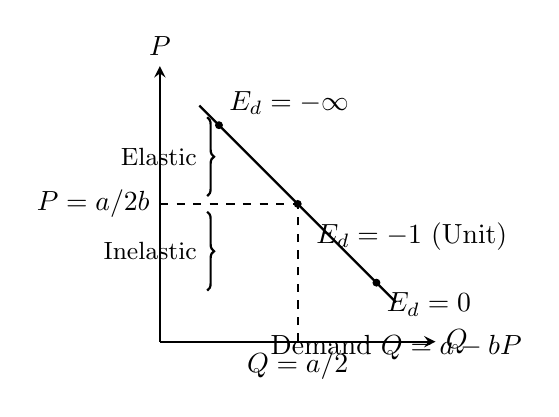
\begin{tikzpicture}[scale=0.5, thick, >=stealth]
    \draw[->] (0,0) -- (7,0) node[right] {$Q$};
    \draw[->] (0,0) -- (0,7) node[above] {$P$};
    \draw[thick] (1,6) -- (6,1) node[below=8pt] {Demand $Q=a-bP$};
    \filldraw (1.5,5.5) circle (2pt) node[above right] {$E_d = -\infty$};
    \filldraw (3.5,3.5) circle (2pt) node[below right=3pt] {$E_d = -1$ (Unit)};
    \filldraw (5.5,1.5) circle (2pt) node[below right] {$E_d = 0$};
    \draw[decorate, decoration=brace] (1.2,5.7) -- (1.2,3.7) node[midway, left] {\small Elastic};
    \draw[decorate, decoration=brace] (1.2,3.3) -- (1.2,1.3) node[midway, left] {\small Inelastic};
    \draw[dashed] (3.5,0) node[below] {$Q=a/2$} -- (3.5,3.5);
    \draw[dashed] (0,3.5) node[left] {$P=a/2b$} -- (3.5,3.5);
\end{tikzpicture}
\end{center}
\textit{Interpretation:} On a straight-line demand curve, elasticity declines as we move down. Upper half: elastic ($|E_d|>1$); Midpoint: unit elastic ($|E_d|=1$); Lower half: inelastic ($0<|E_d|<1$). At vertical intercept, $E_d = -\infty$; at horizontal intercept, $E_d = 0$.

\subsection*{Perfectly Elastic vs. Perfectly Inelastic Demand}
\begin{center}
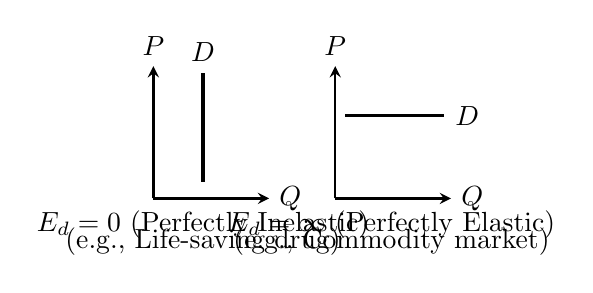
\begin{tikzpicture}[scale=0.42, thick, >=stealth]
    % Perfectly Inelastic
    \draw[->] (0,0) -- (3.5,0) node[right] {$Q$};
    \draw[->] (0,0) -- (0,4) node[above] {$P$};
    \draw[very thick] (1.5,0.5) -- (1.5,3.8) node[above] {$D$};
    \node at (1.5,-0.8) {$E_d = 0$ (Perfectly Inelastic)};
    \node at (1.5,-1.3) {(e.g., Life-saving drug)};
    % Perfectly Elastic
    \draw[->] (5.5,0) -- (9,0) node[right] {$Q$};
    \draw[->] (5.5,0) -- (5.5,4) node[above] {$P$};
    \draw[very thick] (5.8,2.5) -- (8.8,2.5) node[right] {$D$};
    \node at (7.2,-0.8) {$E_d = \infty$ (Perfectly Elastic)};
    \node at (7.2,-1.3) {(e.g., Commodity market)};
\end{tikzpicture}
\end{center}

\subsection*{Total Revenue and Elasticity Relationship}
\begin{center}
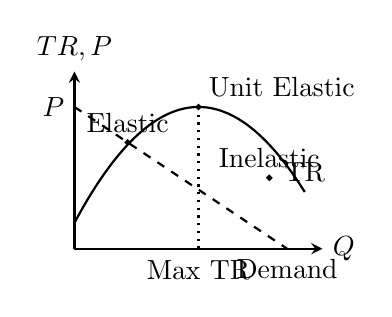
\begin{tikzpicture}[scale=0.45, thick, >=stealth]
    \draw[->] (0,0) -- (7,0) node[right] {$Q$};
    \draw[->] (0,0) -- (0,5) node[above] {$TR, P$};
    % TR curve (inverted U)
    \draw[thick, domain=0:6.5, smooth] plot (\x, {4 - 0.8*(\x-3.5)*(\x-3.5)/3}) node[above] {TR};
    \draw[thick, dashed] (0,4) node[left] {$P$} -- (6,0) node[below] {Demand};
    \filldraw (1.5,3) circle (1.5pt) node[above] {Elastic};
    \filldraw (3.5,4) circle (1.5pt) node[above right] {Unit Elastic};
    \filldraw (5.5,2) circle (1.5pt) node[above] {Inelastic};
    \draw[dotted] (3.5,0) -- (3.5,4);
    \node at (3.5,-0.6) {Max TR};
\end{tikzpicture}
\end{center}
\textit{TR Curve:} Total Revenue ($P \times Q$) reaches maximum at the midpoint (unit elastic point) of a linear demand curve.

% ============================================================================
% PART 5: CALCULATION PROBLEMS AND TECHNIQUES
% ============================================================================
\section*{5. Computing Elasticity -- Detailed Worked Examples}

\subsection*{Example 1: Point Elasticity from Demand Function}
\textbf{Given:} $Q_d = 200 - 4P$. Find $E_d$ at $P = 30$.

\textbf{Solution:}
\begin{enumerate}[leftmargin=*,nosep]
    \item At $P=30$, $Q = 200 - 4(30) = 200 - 120 = 80$.
    \item Derivative: $dQ/dP = -4$.
    \item Point elasticity: $E_d = \frac{dQ}{dP} \cdot \frac{P}{Q} = -4 \cdot \frac{30}{80} = -4 \cdot 0.375 = \mathbf{-1.5}$.
    \item Interpretation: $|E_d| = 1.5 > 1$, demand is \textbf{elastic}. A 1\% price increase leads to a 1.5\% decrease in quantity demanded.
\end{enumerate}

\subsection*{Example 2: Arc Elasticity Calculation}
\textbf{Given:} Price rises from \$10 to \$15, quantity demanded falls from 50 to 30 units.

\textbf{Solution:}
\[
E_d = \frac{(30 - 50) / ((50+30)/2)}{(15 - 10) / ((10+15)/2)} = \frac{-20 / 40}{5 / 12.5} = \frac{-0.5}{0.4} = \mathbf{-1.25}
\]
Interpretation: Over this range, demand is elastic.

\subsection*{Example 3: Income Elasticity from Family Budget Data}
\textbf{Given:} A household's monthly expenditure on meat rises from \$80 to \$96 when monthly income rises from \$2,000 to \$2,400. Calculate income elasticity.

\textbf{Solution:}
\begin{itemize}[leftmargin=*,nosep]
    \item \%$\Delta Q$ = $\frac{96-80}{(96+80)/2} \times 100 = \frac{16}{88} \times 100 = 18.18\%$
    \item \%$\Delta Y$ = $\frac{2400-2000}{(2400+2000)/2} \times 100 = \frac{400}{2200} \times 100 = 18.18\%$
    \item $E_Y = \frac{18.18\%}{18.18\%} = \mathbf{1.0}$ (Unit income elastic -- borderline luxury/necessity).
\end{itemize}

\subsection*{Example 4: Cross Elasticity}
\textbf{Given:} When price of coffee rises from \$4 to \$5 per cup, daily sales of tea increase from 100 to 130 cups. Find $E_{xy}$.

\textbf{Solution:}
\[
\%\Delta Q_{\text{tea}} = \frac{130-100}{(130+100)/2} \times 100 = \frac{30}{115} \times 100 \approx 26.09\%
\]
\[
\%\Delta P_{\text{coffee}} = \frac{5-4}{(5+4)/2} \times 100 = \frac{1}{4.5} \times 100 \approx 22.22\%
\]
\[
E_{xy} = \frac{26.09}{22.22} \approx \mathbf{1.17}
\]
Interpretation: Positive cross elasticity confirms tea and coffee are \textbf{substitutes}. A 1\% rise in coffee price increases tea demand by 1.17\%.

\columnbreak

% ============================================================================
% PART 6: TOTAL REVENUE AND CONSUMER EXPENDITURE PATTERN
% ============================================================================
\section*{6. Elasticity, Total Revenue \& Consumer Expenditure}

\subsection*{The Revenue Test}
Total Revenue ($TR$) = Price $\times$ Quantity = $P \times Q$. The relationship between price change and $TR$ change depends entirely on demand elasticity:

\begin{center}
\begin{tabular}{@{}p{1.5cm}p{2.2cm}p{2.2cm}@{}}
\toprule
\textbf{Elasticity} & \textbf{$P \uparrow$ Effect on $TR$} & \textbf{$P \downarrow$ Effect on $TR$} \\
\midrule
Elastic ($|E_d|>1$) & $TR \downarrow$ & $TR \uparrow$ \\
Unit Elastic ($|E_d|=1$) & $TR$ unchanged & $TR$ unchanged \\
Inelastic ($|E_d|<1$) & $TR \uparrow$ & $TR \downarrow$ \\
\bottomrule
\end{tabular}
\end{center}

\subsection*{Mathematical Proof}
Let $TR = P \cdot Q(P)$. Differentiating with respect to $P$:
\[
\frac{d(TR)}{dP} = Q + P \cdot \frac{dQ}{dP} = Q \left(1 + \frac{P}{Q} \cdot \frac{dQ}{dP}\right) = Q (1 + E_d)
\]
Since $E_d < 0$:
\begin{itemize}[leftmargin=*,nosep]
    \item If $|E_d| > 1$, then $(1+E_d) < 0$, so $d(TR)/dP < 0$: $TR$ falls when $P$ rises.
    \item If $|E_d| < 1$, then $(1+E_d) > 0$, so $d(TR)/dP > 0$: $TR$ rises when $P$ rises.
    \item If $|E_d| = 1$, then $(1+E_d) = 0$, so $d(TR)/dP = 0$: $TR$ is maximized.
\end{itemize}

\subsection*{Consumer Expenditure Pattern}
Consumer expenditure ($E$) on a good = $P \times Q_d$. For normal goods, as price falls, expenditure may rise or fall depending on elasticity:
\begin{itemize}[leftmargin=*,nosep]
    \item \textbf{Elastic goods:} Price cut $\to$ expenditure rises (people buy proportionally more).
    \item \textbf{Inelastic goods:} Price cut $\to$ expenditure falls (people buy only slightly more).
\end{itemize}
This is critical for business pricing strategy: for products with many substitutes (elastic), lowering price increases total sales revenue; for necessities with few alternatives (inelastic), raising price may increase revenue.

\subsection*{Income-Expenditure Patterns (Engel Curve)}
From family budget data, the \textbf{Engel curve} shows relationship between income and expenditure on a good:
\begin{itemize}[leftmargin=*,nosep]
    \item $E_Y > 1$: Share of budget spent on good rises with income (luxuries, e.g., leisure travel).
    \item $0 < E_Y < 1$: Share falls (necessities, e.g., staple food).
    \item $E_Y < 0$: Absolute expenditure falls (inferior goods, e.g., public transport as income rises).
\end{itemize}

% ============================================================================
% PART 7: DETERMINANTS OF ELASTICITY
% ============================================================================
\section*{7. Determinants of Price Elasticity of Demand}

\begin{enumerate}[leftmargin=*,nosep]
    \item \textbf{Availability of Substitutes:} More close substitutes $\to$ higher elasticity (Butter vs. margarine = elastic; Insulin = inelastic). \textit{Most important determinant.}
    \item \textbf{Necessity vs. Luxury:} Necessities (food, water, electricity) tend to be inelastic; luxuries (jewelry, vacation) are elastic.
    \item \textbf{Proportion of Income Spent:} Goods consuming a large fraction of income (housing, cars) are more elastic; small-ticket items (salt, matches) are inelastic.
    \item \textbf{Definition of Market (Breadth):}
    \begin{itemize}[nosep]
        \item Narrowly defined goods (specific brand of rice) have higher elasticity (many substitutes).
        \item Broadly defined categories (all food) have lower elasticity (few substitutes).
    \end{itemize}
    \item \textbf{Time Horizon:} Demand becomes \textbf{more elastic} over time as consumers find alternatives and adjust behavior (short-run gasoline demand is inelastic; long-run, people buy fuel-efficient cars, use transit).
    \item \textbf{Addiction / Habit Formation:} Addictive goods (tobacco, alcohol) tend to have low price elasticity.
    \item \textbf{Durability:} Durable goods (refrigerators, cars) have more elastic demand because purchase can be postponed.
\end{enumerate}

\subsection*{Determinants of Price Elasticity of Supply}
\begin{enumerate}[leftmargin=*,nosep]
    \item \textbf{Time Period:} The most critical factor. \textbf{Momentary supply} (fixed, perfectly inelastic); \textbf{Short-run} (some factors variable, moderately elastic); \textbf{Long-run} (all factors variable, highly elastic).
    \item \textbf{Flexibility of Production:} If resources can be easily shifted in/out (e.g., garment manufacturing), supply is elastic. If specialized capital is needed (e.g., shipbuilding), supply is inelastic.
    \item \textbf{Availability of Inputs:} If inputs are readily available, supply is more elastic.
    \item \textbf{Storage Capacity:} Goods that can be stored cheaply (non-perishables) have more elastic supply; perishables (fresh produce) have inelastic supply.
    \item \textbf{Complexity of Production:} Simple products (textiles) = elastic supply; complex products requiring highly skilled labor (semiconductors) = inelastic supply in short-run.
\end{enumerate}

% ============================================================================
% PART 8: EXTENSIVE CASE STUDIES
% ============================================================================
\section*{8. Comprehensive Case Studies}

\subsection*{Case Study 1: OPEC Oil Price Shocks and the Elasticity of Oil Demand (1973--2023)}

\textbf{Background:} The Organization of Petroleum Exporting Countries (OPEC) is a cartel that controls roughly 40\% of global crude oil production. Understanding the price elasticity of oil demand has been central to predicting cartel power.

\textbf{The 1973 Oil Embargo:} OPEC (Arab members) imposed an oil embargo, sharply cutting supply. Oil prices quadrupled from \$3/barrel to nearly \$12/barrel.

\textbf{Economic Analysis Using Elasticity:}

\textit{Short-Run (1973--1975):}
\begin{itemize}[leftmargin=*,nosep]
    \item \textbf{Demand was highly inelastic ($|E_d| \approx 0.05$ to $0.1$).}
    \item Reasons: No immediate substitutes for gasoline and heating oil; existing stock of cars and furnaces was fuel-inefficient; commuting patterns and housing locations were fixed.
    \item \textbf{Result:} The massive price rise led to only a small decrease in consumption. OPEC revenues soared. The world experienced stagflation -- a supply shock combined with inelastic demand meant high prices without immediate demand adjustment.
\end{itemize}

\textit{Long-Run (1975--1985):}
\begin{itemize}[leftmargin=*,nosep]
    \item \textbf{Demand became more elastic ($|E_d| \approx 0.3$ to $0.5$).}
    \item Reasons: Consumers switched to fuel-efficient Japanese cars; governments mandated Corporate Average Fuel Economy (CAFE) standards; industries adopted energy-saving technologies; home insulation improved; alternative energy (nuclear, coal) expanded.
    \item \textbf{Result:} Oil consumption fell significantly. OPEC's market share and revenue collapsed by the mid-1980s. The price fell below \$10/barrel.
\end{itemize}

\textit{Modern Period (2008--2023):}
\begin{itemize}[leftmargin=*,nosep]
    \item Oil prices spiked to \$147/barrel in 2008, then crashed. The development of fracking technology (shale oil) dramatically increased \textbf{supply elasticity} from non-OPEC sources -- the US became the world's largest producer.
    \item \textbf{Cross-elasticity in action:} Rising oil prices accelerated adoption of electric vehicles (Tesla). EVs are a \textbf{substitute} for gasoline cars. The cross-elasticity of EV demand with respect to gasoline prices is positive and significant ($E_{xy} \approx 0.2$ to $0.4$).
    \item \textbf{2022 Energy Crisis (Russia-Ukraine War):} European natural gas prices surged 5--10 times. Short-run demand for gas was inelastic (winter heating, fixed infrastructure), causing massive expenditure increases for households and industries. Long-run, Europe accelerated renewables and LNG terminals.
\end{itemize}

\textbf{Policy Lesson:} The elasticity of demand determines the effectiveness and consequences of supply shocks. A cartel's long-run power is limited by the long-run demand elasticity being substantially higher than short-run elasticity. Tax/subsidy policies on energy must consider these elasticity dynamics.

\subsection*{Case Study 2: The ``Sin Tax'' -- Cigarette Taxation and Price Elasticity of Demand}

\textbf{Background:} Governments worldwide impose high excise taxes on cigarettes with two objectives: (a) reduce smoking (public health) and (b) raise tax revenue. The effectiveness depends critically on the \textbf{price elasticity of cigarette demand}.

\textbf{The Economic Puzzle:} If demand is inelastic, taxes raise substantial revenue but don't reduce smoking much. If elastic, taxes reduce smoking effectively but raise less revenue. Which is it?

\textbf{Empirical Evidence:}
\begin{itemize}[leftmargin=*,nosep]
    \item \textbf{Adult smokers:} Meta-analyses (Becker, Grossman, Chaloupka) show long-run price elasticity of cigarette demand for adults is approximately $-0.4$ to $-0.6$ (inelastic). A 10\% price increase reduces consumption by 4--6\%.
    \item \textbf{Youth/Teens:} Price elasticity is significantly higher, around $-1.0$ to $-1.4$ (elastic). Young smokers are more price-sensitive due to lower disposable income and less addiction.
    \item \textbf{Income Elasticity:} Cigarettes are an \textbf{inferior good} in developed countries ($E_Y < 0$). As incomes rise, smoking prevalence declines. In developing countries, $E_Y$ may be positive initially.
\end{itemize}

\textbf{Case Study: Australia's Plain Packaging and Tax Hike (2012--2020):}
\begin{itemize}[leftmargin=*,nosep]
    \item Australia imposed plain packaging and raised excise tax annually by 12.5\% (above inflation) from 2013 to 2020. A pack of 25 cigarettes rose from AUD 16 to over AUD 40.
    \item \textbf{Result:} Smoking prevalence fell from 16.1\% (2011--12) to 11.0\% (2019). Daily smokers declined. Government tobacco excise revenue continued to rise despite falling volume because demand is inelastic -- the \textbf{revenue effect} outweighed the quantity effect. Revenue rose from AUD 8.3 billion (2012) to over AUD 17 billion (2019).
    \item \textbf{Deadweight Loss:} Because demand is relatively inelastic, the deadweight loss per dollar of tax raised is smaller than for elastic goods -- making it a relatively ``efficient'' tax from a welfare perspective.
    \item \textbf{Regressive Impact:} Smoking prevalence is higher among lower-income groups. Because demand is inelastic among addicted low-income smokers, the tax burden falls disproportionately on them, raising equity concerns.
    \item \textbf{Illicit Trade:} High taxes create incentives for black market cigarettes. Elasticity of supply of illicit tobacco (highly elastic, mobile) partially offsets the health gains. Australia's extensive border controls limited this.
\end{itemize}

\textbf{Policy Design Implications:}
\begin{enumerate}[leftmargin=*,nosep]
    \item Since youth demand is elastic, price increases are particularly effective at preventing smoking initiation -- a major public health win.
    \item For addicted adult smokers (inelastic demand), complementary policies (cessation support, nicotine replacement therapy) are needed alongside taxes.
    \item Revenue from sin taxes can hypothetically fund health programs, but governments may become dependent on this revenue stream.
    \item Cross-elasticity: As cigarette prices rise, demand for substitutes like e-cigarettes/vaping increases (positive cross-elasticity), creating new regulatory challenges.
\end{enumerate}

\textbf{Economic Concept Summary:} The case demonstrates the power of elasticity analysis in policy -- understanding \textbf{who responds, by how much, and over what time horizon} is essential for predicting outcomes of taxation and designing effective, equitable interventions.

% ============================================================================
% PART 9: EXAM QUESTIONS WITH MODEL ANSWERS
% ============================================================================
\section*{9. Exam Practice Questions \& Detailed Answers}

\subsection*{Question 1: Calculation (Comprehensive)}
\textbf{The demand for a product is given by $Q_d = 500 - 0.5P$.}
\textbf{(a) Find price elasticity at $P = 400$ and $P = 600$. Interpret.}
\textbf{(b) At what price is demand unit elastic?}
\textbf{(c) If the current price is \$400, should the firm raise or lower price to increase total revenue? Explain using elasticity and the total revenue test.}
\textbf{(d) If consumer income increases by 10\% and demand becomes $Q_d = 560 - 0.5P$, calculate the income elasticity of demand at the original price of \$400. Classify the good.}

\vspace{0.1cm}
\textbf{Model Solution:}
\vspace{0.05cm}
\textbf{(a)} $dQ/dP = -0.5$.
\begin{itemize}[nosep]
    \item At $P=400$: $Q = 500 - 0.5(400) = 300$. $E_d = -0.5 \times \frac{400}{300} = -0.667$. $|E_d| = 0.667 < 1$. Demand is \textbf{inelastic}.
    \item At $P=600$: $Q = 500 - 0.5(600) = 200$. $E_d = -0.5 \times \frac{600}{200} = -1.5$. $|E_d| = 1.5 > 1$. Demand is \textbf{elastic}.
\end{itemize}
\textbf{(b)} Unit elastic when $|E_d| = 1$:
$| -0.5 \times \frac{P}{500 - 0.5P} | = 1 \implies 0.5P = 500 - 0.5P \implies P = 500$. At $P=500$, $Q=250$.

\textbf{(c)} At $P=400$, $|E_d| = 0.667 < 1$ (inelastic). With inelastic demand, a price \textbf{increase} will raise Total Revenue ($TR$). $TR$ currently = $400 \times 300 = 120,000$. If $P$ rose to e.g., \$500, $Q=250$, $TR = 125,000$ (higher). The firm should \textbf{raise price}.

\textbf{(d)} At $P=400$, original $Q_1 = 300$, new $Q_2 = 560 - 0.5(400) = 360$.
$\%\Delta Q = \frac{360-300}{(360+300)/2} \times 100 = \frac{60}{330} \times 100 \approx 18.18\%$. $\%\Delta Y = 10\%$.
$E_Y = \frac{18.18}{10} \approx 1.82$. Since $E_Y > 0$ and $> 1$, the good is a \textbf{luxury normal good}.

\vspace{0.2cm}

\subsection*{Question 2: Conceptual Application}
\textbf{Suppose the government imposes a tax on sugary drinks to reduce obesity. Using the concepts of price elasticity of demand and cross-elasticity, explain:}
\textbf{(a) Why the effectiveness of the tax depends on the own-price elasticity of sugary drinks.}
\textbf{(b) Why we must also consider the cross-elasticity with non-sugary drinks and other snacks.}
\textbf{(c) How the tax incidence between consumers and producers relates to elasticity.}

\vspace{0.1cm}
\textbf{Answer:}
\vspace{0.05cm}
\textbf{(a) Effectiveness depends on $E_d$:} The tax raises the price of sugary drinks. The reduction in consumption equals \%$\Delta P \times E_d$. If demand is elastic ($|E_d| > 1$), the quantity consumed falls substantially, achieving health goals. If demand is inelastic ($|E_d| < 1$, e.g., due to addiction/habit), consumption falls only modestly, and the tax primarily raises revenue without significantly changing behavior. Evidence suggests sugary drink demand is moderately elastic ($|E_d| \approx 1.0 - 1.3$), so taxes can be effective.

\textbf{(b) Cross-elasticity matters:} Consumers may substitute away from taxed sugary drinks to \textbf{untaxed alternatives}. If cross-elasticity with diet drinks is positive and high ($E_{xy} \gg 0$), consumers switch to diet sodas -- a positive health outcome. However, if cross-elasticity with other unhealthy goods like sugary snacks or fruit juices (high in natural sugar) is also positive, the net health benefit may be smaller. Cross-elasticity with \textbf{bottled water} is an important policy parameter. If water is a close substitute (high $+E_{xy}$), the tax may have a double benefit -- reduced soda, increased water consumption.

\textbf{(c) Tax incidence:} The burden of the tax falls more heavily on the side of the market that is \textbf{less elastic}. If demand for sugary drinks is relatively inelastic compared to supply, consumers bear most of the tax through higher prices. If supply is inelastic (e.g., limited bottling capacity in short-run), producers bear more. Empirical evidence suggests consumer demand is more inelastic than producer supply (especially given many beverage alternatives in supply), meaning consumers pay the majority of a soda tax.

\vspace{0.2cm}

\subsection*{Question 3: Data Analysis}
\textbf{A household's monthly budget at two income levels is given. Analyze income elasticity and classify each good.}

\begin{center}
\begin{tabular}{@{}lcc@{}}
\toprule
\textbf{Good} & \textbf{Income =\$3,000} & \textbf{Income =\$4,500} \\
\midrule
Food (total) & \$900 & \$1,200 \\
Public Transport & \$200 & \$180 \\
Entertainment & \$150 & \$360 \\
\bottomrule
\end{tabular}
\end{center}

\textbf{Solution:}
\begin{itemize}[leftmargin=*,nosep]
    \item \textbf{Food:} $\%\Delta Q = \frac{300}{1050} \times 100 = 28.57\%$; $\%\Delta Y = \frac{1500}{3750} \times 100 = 40\%$. $E_Y = 28.57/40 = 0.714$. ($0 < E_Y < 1$: \textbf{Necessity}).
    \item \textbf{Public Transport:} $\%\Delta Q = \frac{-20}{190} \times 100 = -10.53\%$. $E_Y = -10.53/40 = -0.263$. ($E_Y < 0$: \textbf{Inferior good} -- as income rises, household spends less on buses, may buy a car).
    \item \textbf{Entertainment:} $\%\Delta Q = \frac{210}{255} \times 100 = 82.35\%$. $E_Y = 82.35/40 = 2.06$. ($E_Y > 1$: \textbf{Luxury}).
\end{itemize}

\vspace{0.2cm}

\subsection*{Question 4: Short Conceptual}
\textbf{Explain why the price elasticity of demand for a specific brand of salt is likely much higher than the elasticity of demand for salt as a whole.}

\textbf{Answer:} A specific brand of salt (e.g., ``Tata Salt'') has many close \textbf{substitutes} -- other branded salts, generic store brands, sea salt, rock salt. If Tata raises its price, consumers easily switch to alternatives, so demand is \textbf{elastic}. Salt as a whole (a broad category) has \textbf{no close substitutes} and constitutes a tiny fraction of consumer income; it is a necessity. Therefore, aggregate salt demand is highly \textbf{inelastic} ($|E_d| \approx 0.1$). This illustrates the principle: \textit{The narrower the market definition, the higher the elasticity}.

\end{multicols}

% ============================================================================
% SINGLE COLUMN SUMMARY TABLE
% ============================================================================
\vspace{0.3cm}
\begin{center}
\fbox{\begin{minipage}{0.9\textwidth}
\footnotesize
\textbf{Summary Cheat Sheet: Elasticity Formulae and Sign Conventions}
\begin{center}
\begin{tabular}{@{}p{2.8cm}p{1.8cm}p{2.2cm}p{2.2cm}@{}}
\toprule
\textbf{Elasticity Type} & \textbf{Formula} & \textbf{Sign} & \textbf{Interpretation} \\
\midrule
Price Elasticity ($E_d$) & $\frac{dQ}{dP} \cdot \frac{P}{Q}$ & Negative ($-$) & $|E_d|>1$ elastic; $<1$ inelastic \\
Income Elasticity ($E_Y$) & $\frac{dQ}{dY} \cdot \frac{Y}{Q}$ & $+$ Normal; $-$ Inferior & $>1$ luxury; $0$--$1$ necessity \\
Cross Elasticity ($E_{xy}$) & $\frac{dQ_x}{dP_y} \cdot \frac{P_y}{Q_x}$ & $+$ Substitutes; $-$ Complements & Magnitude shows strength of relationship \\
Supply Elasticity ($E_s$) & $\frac{dQ_s}{dP} \cdot \frac{P}{Q_s}$ & Positive ($+$) & Higher in long-run \\
Arc Elasticity & $\frac{\Delta Q}{\Delta P} \cdot \frac{P_1+P_2}{Q_1+Q_2}$ & (Depends) & Use for discrete/large changes \\
\bottomrule
\end{tabular}
\end{center}

\vspace{0.1cm}
\textbf{Key Relationships to Remember:}
\begin{itemize}[leftmargin=*,nosep]
    \item $TR$ maximized when $|E_d| = 1$; $MR = P(1 + 1/E_d)$. If $|E_d| > 1$, $MR > 0$; if $|E_d| < 1$, $MR < 0$.
    \item Elasticity varies \textit{along} a linear demand curve; constant only for special forms ($Q = aP^{-b}$).
    \item Engel's Law: As income rises, the proportion of income spent on food falls (food income elasticity $< 1$).
\end{itemize}
\end{minipage}}
\end{center}

\end{document}
\newpage

% ============================================================================
% TOPIC 4: Consumer Behavior and Utility
% ============================================================================
\documentclass[10pt,a4paper]{article}
\usepackage[margin=0.7in]{geometry}
\usepackage{multicol}
\usepackage{amsmath}
\usepackage{tikz}
\usepackage{enumitem}
\usepackage{titlesec}
\usepackage{booktabs}
\usepackage{fontspec}

% Compact formatting
\setlength{\columnsep}{0.7cm}
\setlength{\parindent}{0pt}
\setlength{\parskip}{0.12cm}
\titlespacing{\section}{0pt}{0.4cm}{0.15cm}
\titlespacing{\subsection}{0pt}{0.25cm}{0.08cm}
\titlespacing{\subsubsection}{0pt}{0.2cm}{0.05cm}

% Custom section style
\titleformat{\section}{\large\bfseries}{}{0em}{}
\titleformat{\subsection}{\normalsize\bfseries}{}{0em}{}
\titleformat{\subsubsection}{\normalsize\bfseries\itshape}{}{0em}{}

\begin{document}

\begin{center}
{\LARGE \textbf{Consumer Behavior and Utility Theory}}\\[0.15cm]
{\normalsize \textit{Topic 4: Rational Choice, Utility Maximization, and Welfare}}\\[0.15cm]
\hrule
\end{center}
\vspace{-0.3cm}

\begin{multicols}{2}
\footnotesize

% ============================================================================
% PART 1: DEFINITIONS AND CORE CONCEPTS
% ============================================================================
\section*{1. Definition and Foundational Concepts}

\subsection*{Consumer Behavior}
\textbf{Consumer Behavior} is the study of how individuals make decisions to allocate their limited resources (income, time) among competing goods and services to maximize \textbf{satisfaction} or \textbf{utility}. It forms the microeconomic foundation of the demand curve.

\textbf{Key Questions Addressed:}
\begin{itemize}[leftmargin=*,nosep]
    \item Why does a consumer buy more of a good when its price falls?
    \item How does a consumer choose between two goods given a budget constraint?
    \item What is the welfare gain a consumer receives from market transactions?
\end{itemize}

\subsection*{Utility -- Basic Concept}
\textbf{Utility} ($U$) is the satisfaction, happiness, or pleasure a consumer derives from consuming a good or service. It is a \textbf{subjective} and psychological concept, not an objective physical measure. Economists assume consumers act \textit{as if} they maximize utility.

\textbf{Two Approaches to Measuring Utility:}
\begin{enumerate}[leftmargin=*,nosep]
    \item \textbf{Cardinal Utility:} Utility is \textbf{measurable} in numerical units (``utils''). One can say: ``Bundle A gives 80 utils, Bundle B gives 50 utils, so I prefer A exactly 1.6 times as much.'' This is the classical approach (Marshall, Pigou). Assumes interpersonal comparisons are possible.
    \item \textbf{Ordinal Utility:} Utility is \textbf{not measurable} cardinally; consumers can only \textbf{rank} bundles in order of preference (1st, 2nd, 3rd...). One can say: ``I prefer A to B,'' but not by how much. This is the modern approach (Hicks-Allen, Samuelson). Uses indifference curves and budget lines.
\end{enumerate}

\subsection*{Consumer's Preference Ordering (Ordinal Approach)}
Consumers are assumed to have a rational preference relation $\succsim$ (``at least as good as'') satisfying:
\begin{enumerate}[leftmargin=*,nosep]
    \item \textbf{Completeness:} For any two bundles $A$ and $B$, the consumer can say $A \succsim B$ or $B \succsim A$ (or both, meaning indifference). No indecision.
    \item \textbf{Transitivity:} If $A \succsim B$ and $B \succsim C$, then $A \succsim C$. Preferences are logically consistent.
    \item \textbf{Monotonicity (Non-satiation):} More of a good is always preferred to less (``more is better''), assuming goods are ``goods'' not ``bads.''
    \item \textbf{Convexity:} Averages are preferred to extremes. The consumer prefers a mix of goods rather than extreme bundles (diminishing MRS).
\end{enumerate}

% ============================================================================
% PART 2: MEMORY TRIGGERS
% ============================================================================
\section*{2. How to Remember (Conceptual Anchors)}

\begin{itemize}[leftmargin=*,nosep]
    \item \textbf{Cardinal = Countable (like Calories):} ``Cardinal'' shares root with ``cardinal numbers'' (1, 2, 3...). Think of utils as countable satisfaction points.
    \item \textbf{Ordinal = Order (like Olympic Medals):} You only know Gold > Silver > Bronze, not how much better. Ranking, not measuring.
    \item \textbf{Total Utility (TU) = Total Happiness from all units consumed.} Marginal Utility (MU) = \textbf{Extra} happiness from one \textbf{more} unit. (M for Marginal = More.)
    \item \textbf{Diminishing MU:} The first slice of pizza is heavenly; the 5th slice makes you sick. Each additional unit adds less satisfaction than the previous one.
    \item \textbf{Equimarginal Principle:} Allocate your budget so the ``bang for your buck'' ($MU/P$) is \textbf{equal} across all goods. Mnemonic: ``Balance your bucks for maximum bliss.''
    \item \textbf{Income Effect vs Substitution Effect:}
    \begin{itemize}[nosep]
        \item Price falls $\to$ you feel \textbf{richer} (real income $\uparrow$) $\to$ buy more normal goods = \textbf{Income Effect}.
        \item Price falls $\to$ good is \textbf{cheaper relative} to others $\to$ switch toward it = \textbf{Substitution Effect}.
    \end{itemize}
    \item \textbf{Slutsky Equation:} Total Effect = Substitution Effect (always negative for own-price) + Income Effect (sign depends on normal/inferior good). ``Slutsky Separates the Slopes.''
    \item \textbf{Consumer Surplus = Bargain Joy:} The difference between what you \textit{would} have paid and what you \textit{actually} paid. The area below demand curve, above price. ``The joy of a good deal.''
\end{itemize}

% ============================================================================
% PART 3: MATHEMATICAL FRAMEWORK
% ============================================================================
\section*{3. Mathematical Formulation and Concepts}

\subsection*{Cardinal Utility: Total and Marginal Utility}

Let $U(x)$ be the total utility from consuming $x$ units of a good. \textbf{Marginal Utility} is the additional utility from consuming one more unit:

\[
MU_x = \frac{\Delta TU}{\Delta x} \quad \text{(Discrete)} \qquad MU_x = \frac{dU}{dx} \quad \text{(Continuous)}
\]

\textbf{Relationship between TU and MU:}
\begin{itemize}[leftmargin=*,nosep]
    \item When $MU > 0$, TU is \textbf{increasing}.
    \item When $MU = 0$, TU is at its \textbf{maximum} (satiation point).
    \item When $MU < 0$, TU is \textbf{decreasing} (disutility).
    \item The slope of the TU curve at any point equals the value of MU at that quantity.
\end{itemize}

\textbf{Law of Diminishing Marginal Utility (Gossen's First Law):}
As a consumer consumes successive units of a good, the marginal utility derived from each additional unit eventually \textbf{declines}, \textit{ceteris paribus}.
\[
\frac{d(MU)}{dx} = \frac{d^2 U}{dx^2} < 0
\]
\textit{Example:} The first glass of water when thirsty gives immense satisfaction (high MU); the second gives less; the fifth may give zero or negative MU.

\subsection*{Equimarginal Principle (Gossen's Second Law, Consumer Equilibrium)}

A consumer with income $M$ facing prices $P_x, P_y$ maximizes utility when:
\[
\frac{MU_x}{P_x} = \frac{MU_y}{P_y} = \lambda \quad \text{(Marginal Utility of Money)}
\]
Subject to: $P_x \cdot x + P_y \cdot y = M \quad \text{(Budget Constraint)}$.

\textbf{Intuition:} The last dollar spent on each good must yield the same additional satisfaction. If $MU_x/P_x > MU_y/P_y$, the consumer should reallocate spending from $y$ to $x$ to increase total utility.

\textbf{For $n$ goods:}
\[
\frac{MU_1}{P_1} = \frac{MU_2}{P_2} = \dots = \frac{MU_n}{P_n} = \lambda
\]

\subsection*{Ordinal Utility: Indifference Curves and MRS}

An \textbf{indifference curve} represents all combinations of two goods that give the consumer the same level of utility. \textbf{Marginal Rate of Substitution (MRS)} is the slope of the indifference curve:

\[
MRS_{xy} = -\frac{dy}{dx}\bigg|_{U=\text{const}} = \frac{MU_x}{MU_y}
\]

The consumer maximizes utility where the budget line is \textbf{tangent} to the highest attainable indifference curve:
\[
MRS_{xy} = \frac{P_x}{P_y} \quad \text{and} \quad P_x x + P_y y = M
\]

\subsection*{Substitution Effect, Income Effect, and the Slutsky Equation}

When the price of good $x$ falls ($P_x \downarrow$), two effects occur:

\textbf{(1) Substitution Effect ($\Delta x^s$):} The good is now relatively cheaper. Consumer substitutes \textit{toward} $x$ and away from $y$. This effect is \textbf{always negative} for own-price changes (i.e., consumption of $x$ rises when its price falls).

\textbf{(2) Income Effect ($\Delta x^i$):} The consumer's \textbf{real income} (purchasing power) increases because the same money income can buy more goods. Effect on $x$ depends on good type:
\begin{itemize}[nosep]
    \item \textbf{Normal good:} Income effect is positive ($\uparrow$ real income $\to$ $\uparrow$ consumption $x$). Reinforces substitution effect.
    \item \textbf{Inferior good:} Income effect is negative. Offsets substitution effect.
    \item \textbf{Giffen good:} Negative income effect is so strong it outweighs the substitution effect, leading to upward-sloping demand! (Very rare.)
\end{itemize}

\textbf{The Slutsky Equation (Elasticity Form):}
\[
\underbrace{\frac{\partial x}{\partial P_x}}_{\text{Total Effect}} = \underbrace{\frac{\partial x^c}{\partial P_x}}_{\text{Subst. Effect } (-)} - \underbrace{x \cdot \frac{\partial x}{\partial M}}_{\text{Income Effect}}
\]
Where $x^c$ is compensated (Hicksian) demand. Multiplying both sides by $P_x/x$ gives the elasticity form:
\[
\varepsilon_{xx} = \varepsilon_{xx}^c - s_x \cdot \eta_x
\]
Where:
\begin{itemize}[leftmargin=*,nosep]
    \item $\varepsilon_{xx}$ = Uncompensated (Marshallian) own-price elasticity.
    \item $\varepsilon_{xx}^c$ = Compensated (Hicksian) own-price elasticity (\textbf{always negative}).
    \item $s_x = P_x x / M$ = Budget share of good $x$.
    \item $\eta_x$ = Income elasticity of demand for good $x$.
\end{itemize}

\textbf{From Slutsky equation, compute elasticities:}
If we know compensated elasticity, budget share, and income elasticity, we can derive Marshallian elasticity. For example: Given $\varepsilon_{xx}^c = -1.2$, $s_x = 0.3$, $\eta_x = 0.8$:
\[
\varepsilon_{xx} = -1.2 - (0.3 \times 0.8) = -1.2 - 0.24 = -1.44
\]
(Marshallian demand more elastic than Hicksian because good is normal; income effect reinforces.)

\subsection*{Consumer's Surplus (Marshallian)}

\textbf{Consumer Surplus (CS)} is the difference between the \textbf{maximum amount a consumer is willing to pay} (total utility) and what they \textbf{actually pay} (market price $\times$ quantity).

\[
CS = \int_{0}^{Q^*} P(Q) \, dQ - P^* \cdot Q^*
\]
For a linear demand $P = a - bQ$, with market price $P^*$:
\[
CS = \frac{1}{2} \times (\text{Choke Price} - P^*) \times Q^* = \frac{1}{2} \cdot \frac{(a - P^*)^2}{b}
\]

\textbf{Applications:}
\begin{itemize}[leftmargin=*,nosep]
    \item Measuring welfare gains from trade, price reductions, or new goods.
    \item Evaluating public projects: Cost-Benefit Analysis.
    \item Determining optimal taxation and deadweight loss.
    \item Setting price discrimination strategies (capturing consumer surplus).
\end{itemize}

% ============================================================================
% PART 4: GRAPHICAL ANALYSIS
% ============================================================================
\section*{4. Graphical Illustrations}

\subsection*{Total Utility and Marginal Utility Curves}
\begin{center}
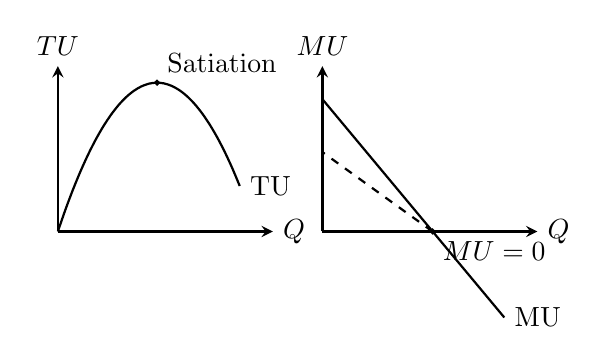
\begin{tikzpicture}[scale=0.42, thick, >=stealth]
    % TU
    \draw[->] (0,0) -- (6.5,0) node[right] {$Q$};
    \draw[->] (0,0) -- (0,5) node[above] {$TU$};
    \draw[thick, domain=0:5.5, smooth] plot (\x, {4 - 1.5*(\x-3)*(\x-3)/3 + 0.5}) node[right] {TU};
    \filldraw (3,4.5) circle (1.5pt) node[above right] {Satiation};
    % MU
    \draw[->] (8,0) -- (14.5,0) node[right] {$Q$};
    \draw[->] (8,0) -- (8,5) node[above] {$MU$};
    \draw[thick, domain=8:13.5, smooth] plot (\x, {4 - 1.2*(\x-8)}) node[right] {MU};
    \filldraw (11.33,0) circle (1.5pt) node[below right] {$MU=0$};
    \draw[dashed] (11.33,0) -- (8,2.4);
\end{tikzpicture}
\end{center}
\textit{Interpretation:} As $Q$ increases, $TU$ rises at a decreasing rate (while $MU>0$), reaches maximum ($MU=0$), then falls ($MU<0$). The $MU$ curve is the derivative (slope) of the $TU$ curve.

\subsection*{Consumer Equilibrium: Cardinal Approach}
\begin{center}
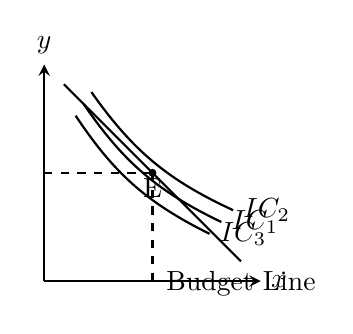
\begin{tikzpicture}[scale=0.5, thick, >=stealth]
    \draw[->] (0,0) -- (5.5,0) node[right] {$x$};
    \draw[->] (0,0) -- (0,5.5) node[above] {$y$};
    \draw[thick] (0.5,5) -- (5,0.5) node[below] {Budget Line};
    \draw[thick] (1,4.5) to[bend right=15] (4.5,1.5) node[right] {$IC_1$};
    \draw[thick] (1.2,4.8) to[bend right=15] (4.8,1.8) node[right] {$IC_2$};
    \draw[thick] (0.8,4.2) to[bend right=15] (4.2,1.2) node[right] {$IC_3$};
    \filldraw (2.75,2.75) circle (2pt);
    \node at (2.75,2.35) {E};
    \draw[dashed] (2.75,0) -- (2.75,2.75);
    \draw[dashed] (0,2.75) -- (2.75,2.75);
\end{tikzpicture}
\end{center}
\textit{At $E$:} $MRS = P_x/P_y$; budget exhausted; consumer on highest attainable indifference curve ($IC_2$).

\subsection*{Substitution and Income Effects (Normal Good)}
\begin{center}
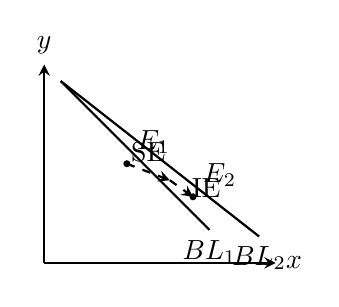
\begin{tikzpicture}[scale=0.42, thick, >=stealth]
    \draw[->] (0,0) -- (7,0) node[right] {$x$};
    \draw[->] (0,0) -- (0,6) node[above] {$y$};
    % Original BL
    \draw (0.5,5.5) -- (5,1) node[below] {$BL_1$};
    % New BL (Px fell)
    \draw (0.5,5.5) -- (6.5,0.8) node[below] {$BL_2$};
    % Tangency points
    \filldraw (2.5,3) circle (2pt) node[above right] {$E_1$};
    \filldraw (4.5,2) circle (2pt) node[above right] {$E_2$};
    % Arrows
    \draw[->, dashed] (2.5,3) -- (3.8,2.5) node[midway, above] {SE};
    \draw[->, dashed] (3.8,2.5) -- (4.5,2) node[midway, right] {IE};
\end{tikzpicture}
\end{center}
\textit{Normal Good:} Total effect ($E_1 \to E_2$) = Substitution Effect (always increases $x$) + Income Effect (also increases $x$).

% ============================================================================
% PART 5: DEEPENED CONCEPTS
% ============================================================================
\section*{5. Deepened Theoretical Concepts}

\subsection*{Slutsky vs. Hicksian Compensation}
\begin{itemize}[leftmargin=*,nosep]
    \item \textbf{Slutsky compensation:} After price change, the consumer is given enough income to buy the \textit{original bundle} at new prices. The substitution effect is measured along a rotated budget line through the original bundle.
    \item \textbf{Hicksian compensation:} After price change, income is adjusted so the consumer remains on the \textit{same indifference curve}. Yields the \textit{pure} substitution effect.
\end{itemize}
For small price changes, both measures converge. Slutsky is observable and used empirically.

\subsection*{Law of Demand: Revisited via Slutsky}
The Law of Demand states: $\partial x / \partial P_x < 0$ (demand curve slopes down). The Slutsky equation shows this holds \textbf{as long as the income effect is not negative and large enough to outweigh the substitution effect}. For a normal good, both effects reinforce -- Law of Demand \textbf{must} hold. For an inferior good, the income effect opposes; if it dominates, we get a \textbf{Giffen good} -- theoretically possible but empirically exceptionally rare.

\subsection*{Consumer's Surplus: Detailed Computation}
For a non-linear demand $Q = f(P)$, consumer surplus is the definite integral:
\[
CS = \int_{P^*}^{P_{\text{max}}} Q(P) \, dP
\]
\textit{Example:} Demand $Q = 100/P^2$. Market price $P^* = 5$, choke price $\infty$ technically, but integrate from 5 to some high value or compute area.

% ============================================================================
% PART 6: EXTENSIVE CASE STUDIES
% ============================================================================
\section*{6. Comprehensive Case Studies}

\subsection*{Case Study 1: The Giffen Good Phenomenon – Potatoes in the Irish Famine (1845--1852)}

\textbf{Background:} During the Great Irish Famine, the staple food of the poor was the potato. When potato prices rose dramatically due to the blight destroying crops, Sir Robert Giffen (and later Alfred Marshall) observed a paradoxical behavior: poor households \textit{increased} their consumption of potatoes as prices rose, contradicting the Law of Demand. This became the classic textbook example of a \textbf{Giffen good}.

\textbf{Economic Mechanism (Detailed Slutsky Decomposition):}

Consider a poor household consuming two goods: \textbf{Potatoes (P)} -- a staple, inferior good that consumes a large share of the budget -- and \textbf{Meat (M)} -- a luxury, normal good.

\textit{Initial Situation:} Household income = \$10/week. Potatoes cost \$1/kg, Meat costs \$5/kg. Baseline consumption: 7 kg potatoes (\$7), 0.6 kg meat (\$3).

\textit{Shock:} Potato blight destroys crops. Potato price rises to \$3/kg.

\textbf{Step 1: Substitution Effect.}
Potatoes are now relatively more expensive compared to meat. Holding real income constant (compensated), the household would substitute \textit{away} from potatoes toward meat. The substitution effect on potato consumption is \textbf{negative}: the household wants fewer potatoes. $\Delta x^s < 0$.

\textbf{Step 2: Income Effect.}
The price increase causes a massive reduction in \textbf{real income}. The household's purchasing power collapses. Before, \$10 bought 7 kg potato + 0.6 kg meat. Now, 7 kg potatoes alone would cost \$21 -- \textbf{more than their entire income}. The household is now substantially poorer.

Because potatoes are an \textbf{inferior good} and consume a very large share of the budget, the income effect is \textbf{positive and very large} (poverty forces the household to buy more inferior staple foods). $\Delta x^i > 0$ and $|\Delta x^i| > |\Delta x^s|$.

\textbf{Step 3: Total Effect.}
\[
\Delta x = \Delta x^s + \Delta x^i
\]
Since $|\Delta x^i| > |\Delta x^s|$, the total effect is \textbf{positive}: $\Delta x > 0$. The household ends up consuming \textit{more} potatoes despite the price rise. Meat becomes completely unaffordable, so the household cuts meat entirely and spends even more of its remaining budget on the now-expensive but still cheapest calorie source: potatoes.

\textbf{Slutsky Equation Application:}
\[
\varepsilon_{PP} = \varepsilon_{PP}^c - s_P \cdot \eta_P
\]
Assume: $\varepsilon_{PP}^c = -0.8$ (compensated elasticity), $s_P = 0.7$ (potatoes are 70\% of budget), $\eta_P = -1.5$ (highly inferior -- income elasticity is negative).
\[
\varepsilon_{PP} = -0.8 - (0.7 \times (-1.5)) = -0.8 + 1.05 = +0.25
\]
Marshallian own-price elasticity is \textbf{positive} ($+0.25$), violating the Law of Demand! A 1\% price increase leads to a 0.25\% \textit{increase} in quantity demanded -- a Giffen good.

\textbf{Conditions for a Giffen Good (All must hold):}
\begin{enumerate}[leftmargin=*,nosep]
    \item The good must be \textbf{strongly inferior} ($\eta < 0$ with large magnitude).
    \item The good must consume a \textbf{large share of the budget} ($s$ must be large).
    \item There must be \textbf{no close substitutes} (otherwise substitution effect would be large).
    \item Applies to poor consumers facing a \textbf{subsistence constraint}.
\end{enumerate}

\textbf{Modern Empirical Evidence:} Jensen and Miller (2008, \textit{American Economic Review}) found evidence of Giffen behavior among extremely poor households in rural China. When the price of rice (staple) was subsidized, households \textit{reduced} rice consumption (as real income rose, they bought more meat). When subsidies were removed and rice price rose, very poor households consumed \textit{more} rice and cut meat consumption. This is the first rigorous empirical confirmation of Giffen behavior.

\textbf{Economic Lesson:} The law of demand is not absolute; it depends on the relative magnitudes of substitution and income effects. Giffen behavior highlights the critical role of income constraints and inferior goods in consumer theory. It also demonstrates why economics distinguishes between theoretical possibilities and empirical regularities.

\subsection*{Case Study 2: Consumer Surplus and the Value of Digital Goods – The Case of Google Search}

\textbf{Background:} Many digital goods (search engines, social media, maps) are provided to consumers at a \textbf{zero monetary price}. GDP and traditional economic metrics fail to capture the value consumers derive from these services because no market transaction occurs. Consumer surplus estimation becomes crucial for measuring welfare in the digital economy.

\textbf{The Problem: How much is ``free'' Google Search worth to consumers?}

\textbf{Methodology: Estimating Consumer Surplus for a Zero-Price Good}

Economists Brynjolfsson, Eggers, and Gannamaneni (2019) used massive online choice experiments to measure the value of digital goods.

\textit{Approach:} They asked representative samples of consumers: ``What is the minimum amount of money you would accept to give up using Google Search for one month?'' This represents the \textbf{compensating variation} -- the income adjustment needed to keep utility unchanged when the good is removed.

\textit{Alternatively:} Infer the demand curve indirectly. Even though the monetary price is zero, the ``full price'' includes \textbf{time costs, attention costs, and privacy costs}. By observing how usage changes with variations in these non-monetary costs (or hypothetical monetary prices in surveys), one can trace out a demand curve.

\textbf{Demand Estimation and Surplus Calculation:}

Assume a survey reveals the following (hypothetical, stylized) demand schedule for Google Search:

\begin{center}
\begin{tabular}{@{ }c@{ }c@{ }}
\toprule
\textbf{Monthly Price (\$)} & \textbf{Users (Millions)} \\
\midrule
\$50  & 10 \\
\$30  & 40 \\
\$20  & 80 \\
\$10  & 150 \\
\$5   & 220 \\
\$0   & 280 \\
\bottomrule
\end{tabular}
\end{center}

\textit{Linear Approximation:} $Q = 280 - 5P$. The choke price (where $Q=0$) is $P_{\text{max}} = 56$.

\[
CS = \int_{0}^{280} \left(56 - \frac{Q}{5}\right) dQ - 0 \times 280 = \frac{1}{2} \times 56 \times 280
\]
\[
CS \approx \mathbf{\$7,840 \text{ million}} = \mathbf{\$7.84 \text{ billion per month}}
\]
Annual consumer surplus from Google Search alone would be on the order of \textbf{\$90+ billion}. This value is \textbf{not captured in GDP} because no transaction occurs. The actual estimates by Brynjolfsson et al. for all free digital goods (search, email, maps, social media) reach several \textbf{hundreds of billions of dollars annually} -- essentially equivalent to a substantial fraction of GDP.

\textbf{Applications and Policy Implications:}
\begin{enumerate}[leftmargin=*,nosep]
    \item \textbf{GDP Mismeasurement:} Massive consumer welfare is generated without any monetary exchange, leading to underestimation of economic well-being and productivity growth in the digital age.
    \item \textbf{Antitrust/Regulation:} If a dominant platform (like Google) were to degrade quality or charge fees, the consumer surplus loss would be enormous. Regulators must weigh this against potential harms when considering break-ups or restrictions.
    \item \textbf{Digital Divide:} Lower-income individuals receive disproportionately large consumer surplus from free digital goods (since they pay zero), reducing effective inequality (real consumption inequality is lower than money-income inequality).
    \item \textbf{Privacy Trade-off:} These services are funded by advertising revenue, which relies on user data. The ``price'' consumers pay is in the form of personal data and attention (non-monetary costs). Consumer surplus analysis must incorporate the \textbf{disutility of privacy loss} as a reduction in net surplus.
    \item \textbf{Cost-Benefit of Internet Access Programs:} Government subsidies for broadband access can be justified by the large consumer surplus generated by access to digital services.
\end{enumerate}

\textbf{Economic Concept Summary:} Consumer surplus is a powerful tool to measure welfare for goods that exist outside traditional markets. In the modern economy, understanding and measuring consumer surplus is increasingly important for policy evaluation, regulation of tech platforms, and assessing real economic well-being beyond GDP metrics.

\columnbreak

% ============================================================================
% PART 7: EXAM QUESTIONS
% ============================================================================
\section*{7. Exam Practice Questions \& Model Answers}

\subsection*{Question 1: Utility Maximization (Cardinal)}
\textbf{A consumer has utility function $U = 10x^{0.5} + 5y$. Prices: $P_x = 2$, $P_y = 4$. Income = \$60.}
\textbf{(a) Find the consumer's optimal consumption bundle.}
\textbf{(b) Verify the equimarginal principle at the optimum.}
\textbf{(c) If $P_x$ falls to \$1, decompose the total change into substitution and income effects.}

\vspace{0.1cm}
\textbf{Solution:}
\textbf{(a)} $MU_x = \frac{10}{2\sqrt{x}} = \frac{5}{\sqrt{x}}$, $MU_y = 5$.
Equimarginal: $\frac{MU_x}{P_x} = \frac{MU_y}{P_y} \Rightarrow \frac{5/\sqrt{x}}{2} = \frac{5}{4} \Rightarrow \frac{5}{2\sqrt{x}} = \frac{5}{4} \Rightarrow 2\sqrt{x} = 4 \Rightarrow \sqrt{x}=2 \Rightarrow \mathbf{x=4}$.
Budget: $2(4) + 4y = 60 \Rightarrow 8 + 4y = 60 \Rightarrow 4y=52 \Rightarrow \mathbf{y=13}$.
Optimal bundle: $\mathbf{(4, 13)}$.

\textbf{(b)} At optimum: $\frac{MU_x}{P_x} = \frac{5/\sqrt{4}}{2} = \frac{2.5}{2} = 1.25$. $\frac{MU_y}{P_y} = \frac{5}{4} = 1.25$. Equal. $\checkmark$

\vspace{0.05cm}
\textbf{(c) New $P_x=1$, New Budget: $x + 4y = 60$.}
New optimum: $\frac{5/\sqrt{x}}{1} = \frac{5}{4} \Rightarrow \frac{5}{\sqrt{x}} = 1.25 \Rightarrow \sqrt{x} = 4 \Rightarrow \mathbf{x=16}$. Budget: $16 + 4y = 60 \Rightarrow 4y=44 \Rightarrow \mathbf{y=11}$. New bundle: $\mathbf{(16, 11)}$.
\textit{Total Effect on x:} $\Delta x = 16 - 4 = +12$.

To decompose: At new prices, find income needed to buy original bundle (Slutsky): $M' = 1(4) + 4(13) = 4 + 52 = 56$. At $M'=56$, find demand: $\frac{5/\sqrt{x}}{1} = \frac{5}{4} \Rightarrow x=16$ (same condition, as demand for $x$ with this utility is independent of income! MU of $y$ is constant, so $x$ depends only on prices). Thus, \textbf{Substitution Effect} = $16 - 4 = 12$. \textbf{Income Effect} = $0$ (because $MU_y$ constant $\to$ quasi-linear utility; all of change is due to price change, none from income). This is a \textbf{zero income effect} good.

\vspace{0.2cm}

\subsection*{Question 2: Slutsky Equation Application}
\textbf{The demand for gasoline is $Q = 100 - 2P$. Original price $P_0 = 10$. New price $P_1 = 15$. Income = \$500.}
\textbf{(a) Calculate the uncompensated (Marshallian) price elasticity at $P_0$.}
\textbf{(b) If the compensated (Hicksian) elasticity is estimated at $-0.2$, and gasoline's budget share is 0.04, what is the implied income elasticity using the Slutsky equation? Is gasoline a normal or inferior good?}

\vspace{0.1cm}
\textbf{Solution:}
\textbf{(a)} At $P_0=10$: $Q = 100 - 2(10) = 80$. $dQ/dP = -2$. $\varepsilon_{xx} = -2 \times (10/80) = \mathbf{-0.25}$.

\textbf{(b)} Slutsky: $\varepsilon_{xx} = \varepsilon_{xx}^c - s_x \cdot \eta_x$.
$-0.25 = -0.2 - 0.04 \cdot \eta_x \Rightarrow -0.05 = -0.04 \cdot \eta_x \Rightarrow \eta_x = \mathbf{1.25}$.
Since $\eta_x > 0$, gasoline is a \textbf{normal good} (more specifically, a luxury since $\eta_x > 1$). The income effect reinforces the substitution effect, making Marshallian demand more elastic ($-0.25$) than Hicksian demand ($-0.2$).

\vspace{0.2cm}

\subsection*{Question 3: Consumer Surplus}
\textbf{Demand for event tickets: $P = 200 - 0.5Q$. Supply is perfectly elastic at $P=50$.}
\textbf{(a) Find equilibrium quantity and consumer surplus.}
\textbf{(b) If the government imposes a tax of \$30 per ticket (suppliers collect), calculate the new consumer surplus, tax revenue, and deadweight loss.}

\vspace{0.1cm}
\textbf{Solution:}
\textbf{(a)} At $P=50$: $50 = 200 - 0.5Q \Rightarrow 0.5Q = 150 \Rightarrow Q^* = 300$.
Choke price: $Q=0 \Rightarrow P=200$. $CS = 0.5 \times (200-50) \times 300 = 0.5 \times 150 \times 300 = \mathbf{\$22,500}$.

\textbf{(b)} \$30 tax shifts supply up to $P=80$ (suppliers must receive 80 to keep 50 after tax). New equilibrium: $80 = 200 - 0.5Q \Rightarrow Q=240$. New $CS = 0.5 \times (200-80) \times 240 = 0.5 \times 120 \times 240 = \mathbf{\$14,400}$.
Tax revenue = $30 \times 240 = \mathbf{\$7,200}$.
Deadweight loss = $0.5 \times 30 \times (300-240) = 0.5 \times 30 \times 60 = \mathbf{\$900}$.
Check: Original $CS$ (22,500) = New $CS$ (14,400) + Tax Revenue (7,200) + DWL (900) = 22,500. $\checkmark$

\vspace{0.2cm}

\subsection*{Question 4: Conceptual}
\textbf{Explain why the substitution effect of a price change is always negative (i.e., quantity demanded moves opposite to the direction of price change), even for Giffen goods.}

\vspace{0.1cm}
\textbf{Answer:} The substitution effect isolates the change in consumption due purely to the change in \textbf{relative prices}, holding real income (utility) constant. When a good becomes relatively cheaper, rationality requires that a consumer substitutes \textit{toward} the now-cheaper good and \textit{away} from relatively more expensive goods to maintain the same utility level. This stems from convexity of indifference curves (diminishing MRS) -- the slope of the curve flattens as we move along it, and tangency with a flatter budget line (due to lower relative price) must occur at a higher quantity of the cheaper good. For a Giffen good, the substitution effect is still negative; however, the income effect is positive (the good is inferior) and so large in magnitude that it dominates the negative substitution effect, creating a positive total effect. The substitution effect itself never violates the law of demand.

\end{multicols}

% ============================================================================
% SUMMARY TABLE
% ============================================================================
\vspace{0.3cm}
\begin{center}
\fbox{\begin{minipage}{0.9\textwidth}
\footnotesize
\textbf{Summary Cheat Sheet: Consumer Theory \& Utility}
\begin{center}
\begin{tabular}{@{}p{3.2cm}p{2.8cm}p{3.2cm}@{}}
\toprule
\textbf{Concept} & \textbf{Formula/Condition} & \textbf{Key Insight} \\
\midrule
Marginal Utility & $MU = \Delta TU / \Delta Q$ & Slope of TU curve \\
Diminishing MU & $d(MU)/dQ < 0$ & Each additional unit adds less satisfaction \\
Equimarginal Principle & $MU_x/P_x = MU_y/P_y$ & Last dollar yields same marginal utility across all goods \\
MRS & $MRS = MU_x/MU_y$ & Slope of indifference curve; willingness to trade \\
Utility Max (Ordinal) & $MRS = P_x/P_y$ & Tangency of BL and IC \\
Slutsky Equation & $\varepsilon = \varepsilon^c - s \cdot \eta$ & Total = Substitution (always $-$) + Income Effect \\
Consumer Surplus & $CS = \int_P^{P_{max}} Q(P)\,dP$ & Welfare measure; area under demand, above price \\
Giffen Good & $\varepsilon > 0$ (positive) & Strong inferior good with large budget share; IE dominates SE \\
\bottomrule
\end{tabular}
\end{center}

\vspace{0.1cm}
\textbf{Quick Sign Summary:}
\begin{itemize}[leftmargin=*,nosep]
    \item Substitution Effect: \textbf{always negative} ($\partial x^c / \partial P_x < 0$).
    \item Income Effect for Normal Good: negative ($-\partial x/\partial M < 0$, so IE negative, reinforces SE).
    \item Income Effect for Inferior Good: positive (offsets SE).
    \item Consumer Surplus increases when price falls; decreases when price rises.
\end{itemize}
\end{minipage}}
\end{center}

\end{document}
\newpage

% ============================================================================
% TOPIC 5: Indifference Curve Analysis
% ============================================================================
\documentclass[10pt,a4paper]{article}
\usepackage[margin=0.7in]{geometry}
\usepackage{multicol}
\usepackage{amsmath}
\usepackage{tikz}
\usepackage{enumitem}
\usepackage{titlesec}
\usepackage{booktabs}
\usepackage{fontspec}

% Compact formatting
\setlength{\columnsep}{0.7cm}
\setlength{\parindent}{0pt}
\setlength{\parskip}{0.12cm}
\titlespacing{\section}{0pt}{0.4cm}{0.15cm}
\titlespacing{\subsection}{0pt}{0.25cm}{0.08cm}
\titlespacing{\subsubsection}{0pt}{0.2cm}{0.05cm}

% Custom section style
\titleformat{\section}{\large\bfseries}{}{0em}{}
\titleformat{\subsection}{\normalsize\bfseries}{}{0em}{}
\titleformat{\subsubsection}{\normalsize\bfseries\itshape}{}{0em}{}

\begin{document}

\begin{center}
{\LARGE \textbf{The Indifference Curve Analysis}}\\[0.15cm]
{\normalsize \textit{Topic 5: Ordinal Utility, Consumer Equilibrium, and Comparative Statics}}\\[0.15cm]
\hrule
\end{center}
\vspace{-0.3cm}

\begin{multicols}{2}
\footnotesize

% ============================================================================
% PART 1: DEFINITION AND INTRODUCTION
% ============================================================================
\section*{1. Definition and Core Concepts}

\subsection*{Indifference Curve Analysis}
\textbf{Indifference Curve Analysis} is a method of analyzing consumer behavior based on \textbf{ordinal utility}. It was developed by \textbf{J.R. Hicks} and \textbf{R.G.D. Allen} (1934) as an improvement over the \textbf{Marshallian cardinal utility} approach. Instead of measuring utility in absolute numerical units (utils), it uses \textbf{indifference curves} and \textbf{budget lines} to study consumer equilibrium through rankings of preference.

\textbf{An Indifference Curve (IC)} is a locus of points representing different combinations of two goods that yield the \textbf{same level of total satisfaction} (utility) to the consumer, making the consumer \textbf{indifferent} among them.

\[
\text{Along an IC: } U(x, y) = \text{constant}
\]

\subsection*{Why Improvement Over Marshallian Analysis?}
\begin{enumerate}[leftmargin=*,nosep]
    \item \textbf{No Need to Measure Utility Cardinally:} Marshall required utility to be measurable in cardinal numbers (1, 2, 3 utils). Hicks-Allen only requires the ability to rank bundles (ordinal). More realistic.
    \item \textbf{No Assumption of Constant Marginal Utility of Money:} Marshall assumed $MU_{\text{money}}$ is constant, which is unrealistic (especially when prices change). Indifference curve analysis does not require this.
    \item \textbf{Decomposes Price Effect:} Marshall could not separate the \textbf{substitution effect} from the \textbf{income effect}. Hicks-Allen explicitly decomposes the total price effect into these two components.
    \item \textbf{Handles Multiple Goods:} The ordinal framework naturally extends to $n$ goods using utility functions and indifference maps.
    \item \textbf{More General:} The law of diminishing marginal utility is replaced by the \textbf{diminishing marginal rate of substitution}, which is a weaker and more intuitive assumption.
\end{enumerate}

\textbf{Underlying Assumptions:}
\begin{itemize}[leftmargin=*,nosep]
    \item Consumer is \textbf{rational} and aims to maximize satisfaction.
    \item Consumer has a consistent and complete \textbf{preference ordering} (completeness, transitivity, reflexivity).
    \item \textbf{Non-satiation:} More of a good is preferred to less.
    \item \textbf{Diminishing MRS:} Indifference curves are convex to the origin.
    \item Goods are \textbf{divisible} and substitutable.
\end{itemize}

% ============================================================================
% PART 2: HOW TO REMEMBER
% ============================================================================
\section*{2. Memory Triggers and Conceptual Anchors}

\begin{itemize}[leftmargin=*,nosep]
    \item \textbf{Indifference Curve = ``Happiness Contour Line'':} Think of a topographic map: each contour line connects points of equal elevation. Here, each IC connects bundles of equal satisfaction. Moving to a higher IC is like climbing a ``happiness mountain.''
    \item \textbf{Properties -- Remember ``C-NOT-C''}: \textbf{C}onvex to origin; \textbf{N}ever intersect; \textbf{O}rdered (higher IC = higher utility); \textbf{T}ouches neither axis (usually); \textbf{C}annot be thick.
    \item \textbf{MRS = Slope of IC:} The Marginal Rate of Substitution tells you how many units of $y$ a consumer willingly gives up to get \textbf{one more unit of $x$} while staying equally happy. Mnemonic: ``My Rate of Swapping.''
    \item \textbf{Diminishing MRS = IC Bow Shape:} As you slide down the curve (getting more $x$), you value additional $x$ less and less, so you're willing to give up fewer and fewer $y$. This ``bowed-in'' shape = convexity.
    \item \textbf{Equilibrium = Tangency:} $MRS = P_x/P_y$. The subjective rate of trade (slope of IC) equals the market rate of trade (slope of budget line). If they differ, you can trade in the market to reach a higher IC. Mnemonic: ``Tangency = Tranquility (no incentive to change).''
    \item \textbf{Budget Line = Affordability Frontier:} Slope $= -P_x/P_y$. The relative price ratio is the opportunity cost of $x$ in terms of $y$ on the market.
    \item \textbf{Income Change = Parallel Shift:} More income shifts the budget line outward parallelly. The path traced by equilibria = \textbf{Income Consumption Curve (ICC)} or Engel curve.
    \item \textbf{Price Change = Rotation:} A fall in $P_x$ rotates the budget line outward from the $y$-intercept. Path of equilibria = \textbf{Price Consumption Curve (PCC)}. From PCC, we derive the demand curve.
\end{itemize}

% ============================================================================
% PART 3: MATHEMATICAL FRAMEWORK
% ============================================================================
\section*{3. Mathematical Formulation}

\subsection*{Utility Function and Indifference Curve}
For a utility function $U = U(x, y)$, an indifference curve for utility level $U_0$ is:
\[
U(x, y) = U_0
\]
Totally differentiating:
\[
\frac{\partial U}{\partial x} dx + \frac{\partial U}{\partial y} dy = 0 \quad \Rightarrow \quad MU_x \, dx + MU_y \, dy = 0
\]

\subsection*{Marginal Rate of Substitution (MRS)}
The \textbf{slope} of the indifference curve (in absolute value) is the MRS:
\[
MRS_{xy} = -\frac{dy}{dx}\bigg|_{U=\text{const}} = \frac{MU_x}{MU_y}
\]
The MRS measures the number of units of $y$ the consumer is willing to sacrifice for one additional unit of $x$, keeping utility constant.

\textbf{Diminishing MRS:}
\[
\frac{d(MRS)}{dx} < 0
\]
As $x$ increases (and $y$ decreases along IC), $MU_x$ falls and $MU_y$ rises (due to diminishing marginal utility), so $MRS = MU_x/MU_y$ declines. Geometrically, the IC is \textbf{convex to the origin}.

\subsection*{Budget Constraint}
\[
P_x \cdot x + P_y \cdot y = M
\]
Slope of budget line: $-\frac{P_x}{P_y}$.

\subsection*{Consumer Equilibrium (Tangency Condition)}
Maximize $U(x,y)$ subject to $P_x x + P_y y = M$. Lagrangian:
\[
\mathcal{L} = U(x,y) + \lambda (M - P_x x - P_y y)
\]
First-order conditions:
\[
\frac{\partial \mathcal{L}}{\partial x} = MU_x - \lambda P_x = 0 \quad (1)
\]
\[
\frac{\partial \mathcal{L}}{\partial y} = MU_y - \lambda P_y = 0 \quad (2)
\]
\[
\frac{\partial \mathcal{L}}{\partial \lambda} = M - P_x x - P_y y = 0 \quad (3)
\]
From (1) and (2):
\[
\frac{MU_x}{MU_y} = \frac{P_x}{P_y} \quad \Rightarrow \quad MRS_{xy} = \frac{P_x}{P_y}
\]
\textbf{Equilibrium Condition:} Slope of indifference curve (MRS) equals slope of budget line (price ratio). Also, the budget must be exhausted.

\subsection*{Corner Solutions}
If MRS never equals price ratio within the feasible range, the consumer maximizes utility at a \textbf{corner} (consuming only one good). Condition:
\[
\frac{MU_x}{P_x} > \frac{MU_y}{P_y} \text{ at } y=0 \quad \Rightarrow \quad \text{Only } x \text{ consumed.}
\]

% ============================================================================
% PART 4: PROPERTIES OF INDIFFERENCE CURVES
% ============================================================================
\section*{4. Properties of Indifference Curves (Detailed)}

\begin{enumerate}[leftmargin=*,nosep]
    \item \textbf{Indifference Curves Slope Downward (Negative Slope):} To keep utility constant, an increase in one good must be compensated by a decrease in the other. If both increase, utility rises (monotonicity). $\to$ Slope is negative.
    \item \textbf{Higher IC Represents Higher Utility:} Due to non-satiation (more is better), bundles on ICs farther from the origin contain more of at least one good (and no less of any), hence higher utility.
    \item \textbf{Indifference Curves Cannot Intersect:} Proof by contradiction: Suppose $IC_1$ and $IC_2$ intersect at point A. Since B is on $IC_1$ and C is on $IC_2$, by transitivity, B and C should be on the same indifference curve if A is common, but they yield different utilities. This violates \textbf{consistency and transitivity} of preferences.
    \item \textbf{Convexity to the Origin:} Due to \textbf{diminishing MRS}. As the consumer moves rightward along the IC (more $x$, less $y$), the willingness to give up $y$ for additional $x$ decreases. The slope flattens. This reflects a \textbf{preference for variety} (balanced bundles preferred to extremes).
    \item \textbf{Indifference Curves Are Not Necessarily Parallel:} MRS may change at different rates across different utility levels, so spacing between curves may vary.
    \item \textbf{Indifference Curves Do Not Touch the Axes (Usually):} In standard analysis with two goods both desired, the consumer always prefers some positive amount of each. However, for perfect substitutes or cases leading to corner solutions, ICs may touch axes.
\end{enumerate}

% ============================================================================
% PART 5: GRAPHICAL ANALYSIS
% ============================================================================
\section*{5. Graphical Illustrations}

\subsection*{Indifference Map and Budget Line}
\begin{center}
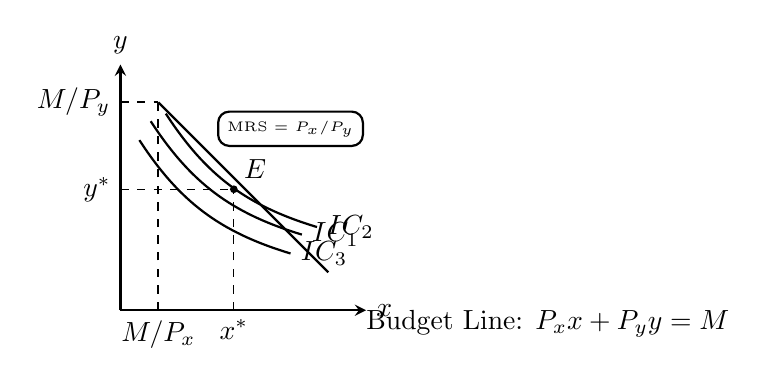
\begin{tikzpicture}[scale=0.48, thick, >=stealth]
    \draw[->] (0,0) -- (6.5,0) node[right] {$x$};
    \draw[->] (0,0) -- (0,6.5) node[above] {$y$};
    % Budget Line
    \draw[thick] (1,5.5) -- (5.5,1) node[below right=10pt] {Budget Line: $P_x x + P_y y = M$};
    \draw[dashed] (1,0) node[below] {$M/P_x$} -- (1,5.5);
    \draw[dashed] (0,5.5) node[left] {$M/P_y$} -- (1,5.5);
    % Indifference curves
    \draw[thick] (0.8,5) to[bend right=20] (4.8,2) node[right] {$IC_1$};
    \draw[thick] (1.2,5.2) to[bend right=20] (5.2,2.2) node[right] {$IC_2$};
    \draw[thick] (0.5,4.5) to[bend right=20] (4.5,1.5) node[right] {$IC_3$};
    % Equilibrium point E
    \filldraw (3,3.2) circle (2pt) node[above right] {$E$};
    \draw[dashed, thin] (3,0) node[below] {$x^*$} -- (3,3.2);
    \draw[dashed, thin] (0,3.2) node[left] {$y^*$} -- (3,3.2);
    \node[draw, fill=white, rounded corners, font=\tiny] at (4.5,4.8) {MRS = $P_x/P_y$};
\end{tikzpicture}
\end{center}
\textit{At $E$, the budget line is tangent to the highest attainable indifference curve ($IC_2$). $IC_3$ is unattainable; $IC_1$ is suboptimal. $MRS = P_x/P_y$.}

\subsection*{Consumer Equilibrium: Corner Solution}
\begin{center}
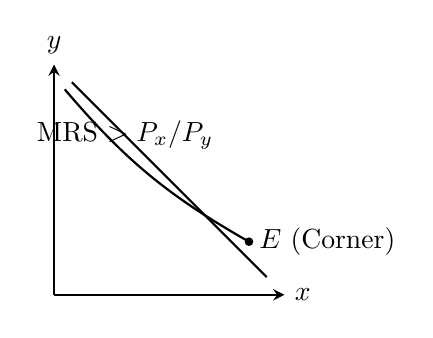
\begin{tikzpicture}[scale=0.45, thick, >=stealth]
    \draw[->] (0,0) -- (6.5,0) node[right] {$x$};
    \draw[->] (0,0) -- (0,6.5) node[above] {$y$};
    \draw (0.5,6) -- (6,0.5);
    \draw[thick] (0.3,5.8) to[bend right=10] (5.5,1.5);
    \filldraw (5.5,1.5) circle (2.5pt) node[right] {$E$ (Corner)};
    \node at (2,4.5) {MRS $> P_x/P_y$};
\end{tikzpicture}
\end{center}
\textit{Corner solution: Consumer spends all income on $x$ because $MU_x/P_x > MU_y/P_y$ everywhere, including at $y=0$. Indifference curve is flatter than budget line at the boundary.}

\subsection*{Income Consumption Curve (ICC) -- Normal Goods}
\begin{center}
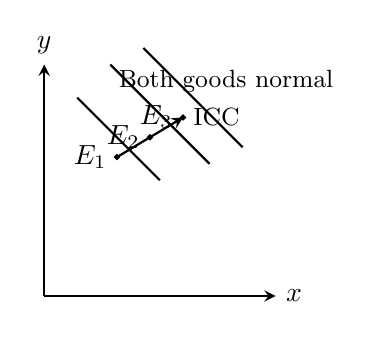
\begin{tikzpicture}[scale=0.42, thick, >=stealth]
    \draw[->] (0,0) -- (7,0) node[right] {$x$};
    \draw[->] (0,0) -- (0,7) node[above] {$y$};
    \draw (1,6) -- (3.5,3.5); \draw (2,7) -- (5,4);
    \draw (3,7.5) -- (6,4.5);
    \filldraw (2.2,4.2) circle (1.5pt) node[left] {$E_1$};
    \filldraw (3.2,4.8) circle (1.5pt) node[left] {$E_2$};
    \filldraw (4.2,5.4) circle (1.5pt) node[left] {$E_3$};
    \draw[thick, ->] (2.2,4.2) -- (3.2,4.8) -- (4.2,5.4) node[right] {\small ICC};
    \node at (5.5,6.5) {\small Both goods normal};
\end{tikzpicture}
\end{center}
\textit{ICC traces equilibrium points as income rises. Upward sloping $\to$ both goods are normal.}

\subsection*{Price Consumption Curve (PCC) and Derivation of Demand}
\begin{center}
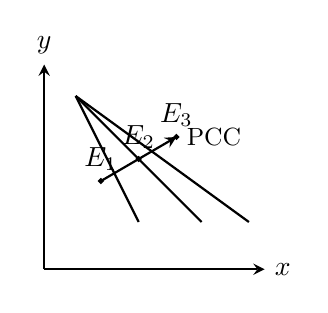
\begin{tikzpicture}[scale=0.4, thick, >=stealth]
    \draw[->] (0,0) -- (7,0) node[right] {$x$};
    \draw[->] (0,0) -- (0,6.5) node[above] {$y$};
    \draw (1,5.5) -- (3,1.5); \draw (1,5.5) -- (5,1.5);
    \draw (1,5.5) -- (6.5,1.5);
    \filldraw (1.8,2.8) circle (1.5pt) node[above] {$E_1$};
    \filldraw (3,3.5) circle (1.5pt) node[above] {$E_2$};
    \filldraw (4.2,4.2) circle (1.5pt) node[above] {$E_3$};
    \draw[thick, ->] (1.8,2.8) -- (3,3.5) -- (4.2,4.2) node[right] {\small PCC};
\end{tikzpicture}
\end{center}
\textit{PCC (or Offer Curve) traces equilibria as $P_x$ falls. From PCC, by plotting $P_x$ against $x^*$, we derive the Marshallian demand curve for $x$.}

\columnbreak

% ============================================================================
% PART 6: EFFECTS OF INCOME AND PRICE CHANGES
% ============================================================================
\section*{6. Income and Price Change Effects}

\subsection*{Income Effect (Income Change)}
When consumer's money income $M$ increases (prices constant), the budget line shifts \textbf{outward parallelly}. The new equilibrium occurs on a higher IC. The line joining equilibria at different income levels is the \textbf{Income Consumption Curve (ICC)}. From ICC, we derive the \textbf{Engel Curve}, showing relationship between income and quantity consumed.

\textbf{Classification by Good Type:}
\begin{itemize}[leftmargin=*,nosep]
    \item \textbf{Normal Good:} ICC slopes upward (both $x$ and $y$ rise with income). Engel curve has positive slope.
    \item \textbf{Inferior Good:} ICC bends backward (consumption of the inferior good falls as income rises, while the other good increases). Engel curve has negative slope beyond a certain income.
    \item \textbf{Luxury Good:} Consumption rises more than proportionately to income.
    \item \textbf{Necessity:} Consumption rises less than proportionately to income.
\end{itemize}

\subsection*{Price Effect (Price Change)}
When $P_x$ falls ($P_y$ and $M$ constant), the budget line \textbf{rotates outward} around the $y$-intercept. The $y$-intercept ($M/P_y$) remains unchanged; the $x$-intercept ($M/P_x$) increases. The line joining equilibria at different prices of $x$ is the \textbf{Price Consumption Curve (PCC)}.

\textbf{Total Price Effect Decomposition (Hicksian Method):}
For a fall in $P_x$:
\begin{enumerate}[leftmargin=*,nosep]
    \item \textbf{Total Effect (TE):} Movement from original equilibrium $E_1$ to final equilibrium $E_2$. $\Delta x = x_2 - x_1$.
    \item \textbf{Substitution Effect (SE):} Draw a hypothetical budget line parallel to the new budget line but tangent to the \textit{original indifference curve}. This removes the income effect (compensated). Movement from $E_1$ to $E_c$ (compensated point). $SE = x_c - x_1$. \textbf{Always positive} (for a price fall, consumption of the cheaper good rises).
    \item \textbf{Income Effect (IE):} Movement from $E_c$ to $E_2$. $IE = x_2 - x_c$. Sign depends on whether the good is normal (positive IE) or inferior (negative IE).
\end{enumerate}
\[
TE = SE + IE \quad \Rightarrow \quad \Delta x = \Delta x^s + \Delta x^i
\]

\subsection*{Graphical Decomposition for Normal Good ($P_x \downarrow$)}
\begin{center}
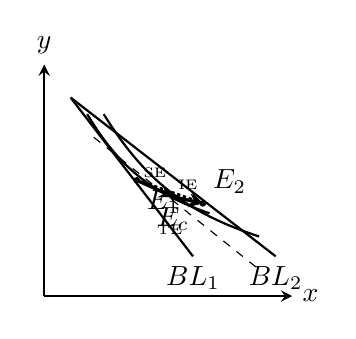
\begin{tikzpicture}[scale=0.42, thick, >=stealth]
    \draw[->] (0,0) -- (7.5,0) node[right] {$x$};
    \draw[->] (0,0) -- (0,7) node[above] {$y$};
    % Original BL
    \draw (0.8,6) -- (4.5,1.2) node[below] {$BL_1$};
    % New BL (Px fell)
    \draw (0.8,6) -- (7,1.2) node[below] {$BL_2$};
    % Hypothetical compensated BL
    \draw[dashed, thin] (1.5,4.8) -- (6.5,0.8);
    % ICs (bowed toward origin)
    \draw (1.3,5.5) to[bend right=20] (5,2.5); % IC1
    \draw (1.8,5.5) to[bend right=20] (6.5,1.8); % IC2
    % Points
    \filldraw (2.8,3.5) circle (1.8pt) node[below right] {$E_1$};
    \filldraw (4.8,2.8) circle (1.8pt) node[above right] {$E_2$};
    \filldraw (3.9,3) circle (1.8pt) node[below] {$E_c$};
    % Arrows
    \draw[->, very thick] (2.8,3.5) -- (3.9,3) node[midway, above] {\tiny SE};
    \draw[->, very thick] (3.9,3) -- (4.8,2.8) node[midway, above] {\tiny IE};
    \draw[->, very thick, densely dotted] (2.8,3.5) -- (4.8,2.8) node[midway, below=8pt] {\tiny TE};
\end{tikzpicture}
\end{center}
\textit{$TE = SE + IE$. For a normal good, both SE and IE work in same direction.}

\subsection*{Special Cases}
\begin{itemize}[leftmargin=*,nosep]
    \item \textbf{Inferior Good ($P_x \downarrow$):} SE positive (increase $x$), IE negative (decrease $x$, because income effect makes consumer feel richer and buy less of inferior good). TE sign ambiguous: if $|SE| > |IE|$, net demand rises (normal demand); if $|IE| > |SE|$, \textbf{Giffen good}, demand falls.
    \item \textbf{Perfect Substitutes:} Straight-line ICs. MRS constant. Equilibrium typically at a corner (consume only cheaper good). No interior tangency unless slopes are equal.
    \item \textbf{Perfect Complements:} L-shaped ICs. MRS not defined at the kink. Consumer always consumes goods in fixed proportions. Income expansion path is a ray from origin. Price change yields only an income effect (no substitution effect, because goods must be consumed together).
\end{itemize}

% ============================================================================
% PART 7: COMPARISON WITH MARSHALLIAN ANALYSIS
% ============================================================================
\section*{7. Indifference Curve vs. Marshallian Utility Analysis}

\begin{center}
\begin{tabular}{@{}p{2.8cm}p{2.8cm}@{}}
\toprule
\textbf{Marshallian (Cardinal)} & \textbf{Hicks-Allen (Ordinal)} \\
\midrule
Utility measurable in utils & Utility only ranked (ordinal) \\
Assumes constant MU of money & No such assumption \\
Law of Diminishing MU & Diminishing MRS (weaker) \\
Single-good analysis focus & Two-good (or multi-good) \\
Cannot separate IE and SE & Explicitly decomposes IE \& SE \\
Budget constraint implicit & Budget line explicit \\
Demand derived from MU = Price & Demand derived from MRS = Price Ratio \\
Substitution effect not isolated & Substitution effect via compensated budget \\
\bottomrule
\end{tabular}
\end{center}

\textbf{Advantage of Indifference Curve:} More general, fewer restrictive assumptions, better analytical tool for welfare, taxation, and policy analysis. The ordinal approach underpins all modern microeconomic consumer theory.

% ============================================================================
% PART 8: EXTENSIVE CASE STUDIES
% ============================================================================
\section*{8. Comprehensive Case Studies}

\subsection*{Case Study 1: Cash vs. In-Kind Transfers -- The Food Stamp Program (US SNAP)}

\textbf{Background:} Governments provide assistance to low-income households either through \textbf{cash transfers} (direct money) or \textbf{in-kind transfers} (specific goods like food stamps, housing vouchers). The US Supplemental Nutrition Assistance Program (SNAP, formerly Food Stamps) provides vouchers that can only be spent on food. Economists have long debated whether cash would be superior using indifference curve analysis.

\textbf{The Economic Question:} Given a fixed government expenditure, which type of transfer provides greater consumer satisfaction (higher utility)?

\textbf{Indifference Curve Analysis Setup:}
Two goods: \textbf{Food (F)} on x-axis, \textbf{All Other Goods (AOG)} on y-axis.

\textit{Initial Situation (No Transfer):} Budget line $BL_0$ with intercepts $M/P_F$ and $M/P_{AOG}$. Equilibrium at $E_0$ on $IC_0$.

\textit{Cash Transfer of Amount \$T:} Income increases by \$T. Budget line shifts outward parallelly from $BL_0$ to $BL_{\text{cash}}$. New equilibrium $E_{\text{cash}}$ on $IC_{\text{cash}}$.

\textit{In-Kind Transfer (Food Stamps of Value \$T, usable only for Food):} The budget line shifts rightward only for food. It becomes \textbf{kinked}: For food quantities up to \$T/$P_F$, the consumer can get them using stamps without sacrificing AOG (the budget line is horizontal at $y = M/P_{AOG}$ for $F \leq \text{stamp quantity}$). Beyond that, the budget line slopes down as usual.

\begin{center}
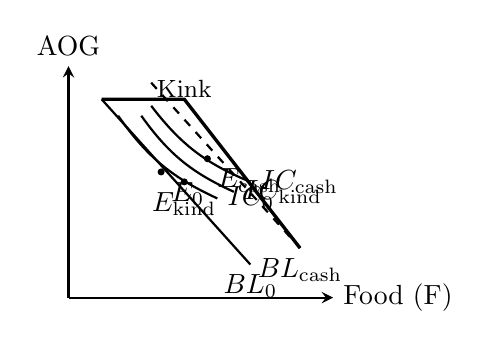
\begin{tikzpicture}[scale=0.42, thick, >=stealth]
    \draw[->] (0,0) -- (8,0) node[right] {Food (F)};
    \draw[->] (0,0) -- (0,7) node[above] {AOG};
    % Original BL
    \draw (1,6) -- (5.5,1) node[below] {$BL_0$};
    % Cash BL
    \draw[dashed] (2.5,6.5) -- (7,1.5) node[below] {$BL_{\text{cash}}$};
    % In-kind kinked BL
    \draw[very thick] (1,6) -- (3.5,6) -- (7,1.5);
    \node at (3.5,6.3) {\small Kink};
    % ICs
    \draw (1.5,5.5) to[bend right=15] (4.5,3) node[right] {$IC_0$};
    \draw (2.5,5.8) to[bend right=15] (5.5,3.5) node[right] {$IC_{\text{cash}}$};
    \draw (2.2,5.5) to[bend right=15] (5,3.2) node[right] {$IC_{\text{kind}}$};
    % Equilibrium points
    \filldraw (2.8,3.8) circle (2pt) node[below right] {$E_0$};
    \filldraw (4.2,4.2) circle (2pt) node[below right] {$E_{\text{cash}}$};
    \filldraw (3.5,3.5) circle (2pt) node[below] {$E_{\text{kind}}$};
\end{tikzpicture}
\end{center}

\textbf{Analysis of Outcomes:}

\textbf{Case A: Consumer Initially Buys Less Food Than Stamp Value.}
The consumer's optimal choice with stamps is at the kink (or beyond where the cash-equivalent BL is available). The in-kind transfer forces the consumer to a point on a \textbf{lower indifference curve} ($IC_{\text{kind}}$) than with cash ($IC_{\text{cash}}$). The consumer would prefer cash because they could allocate spending to more valued AOG rather than being forced to over-consume food relative to their preferences. \textbf{Cash is Pareto-superior} -- it gives the consumer the option to choose the same bundle as with stamps, but also others that yield higher utility.

\textbf{Case B: Consumer Initially Buys More Food Than Stamp Value.}
If the consumer already consumed more food than the stamp quantity, the in-kind transfer is \textbf{equivalent to cash} (the extra stamps simply free up money that would have been spent on food, which is then spent on AOG). The consumer reaches the same $IC_{\text{cash}}$. In this case, the restriction is non-binding.

\textbf{Empirical Evidence and Policy Implications:}
\begin{itemize}[leftmargin=*,nosep]
    \item Studies show most SNAP recipients are \textbf{infra-marginal} (Case B: their food spending exceeds the voucher amount), so the distortion is small for them.
    \item However, \textbf{marginal recipients} (new entrants, those with higher AOG preferences) would indeed be better off with cash.
    \item \textbf{Paternalism:} Policymakers often prefer in-kind transfers to ensure the money is spent on ``merit goods'' (food, housing, education) rather than ``temptation goods'' (alcohol, tobacco). This is a normative judgment overriding consumer sovereignty.
    \item \textbf{Political Economy:} Taxpayers may be more willing to fund food stamps than cash transfers, perceiving less ``waste.'' This political feasibility can make in-kind transfers more generous than cash, potentially making even recipients better off despite the distortion.
    \item The analysis demonstrates how indifference curves can evaluate \textbf{welfare effects of government policy} beyond simple cost analysis.
\end{itemize}

\textbf{Economic Lesson:} Indifference curve analysis provides a rigorous framework for comparing policy instruments. While cash is generally more efficient (higher utility per dollar spent), in-kind transfers may be justified on paternalistic or political grounds. The binding vs. non-binding constraint distinction is critical.

\subsection*{Case Study 2: Work-Leisure Choice and the Backward-Bending Labor Supply Curve}

\textbf{Background:} The labor supply decision involves a trade-off between two ``goods'': \textbf{Income} (consumption of goods) and \textbf{Leisure} (time not working). Indifference curve analysis explains why an increase in the wage rate may either increase or decrease hours worked, leading to a \textbf{backward-bending labor supply curve}.

\textbf{The Model:}
\begin{itemize}[leftmargin=*,nosep]
    \item \textbf{Goods on axes:} Leisure ($L$) on x-axis (hours per day), Income ($Y$) on y-axis.
    \item \textbf{Time Constraint:} $L + H = T$, where $H$ = hours worked, $T$ = total time endowment (e.g., 24 hours/day).
    \item \textbf{Budget Constraint:} $Y = w \cdot H = w (T - L)$. Slope $= -w$ (the wage rate is the opportunity cost of an hour of leisure).
    \item \textbf{Utility:} $U = U(Y, L)$. Leisure is a normal good (usually).
\end{itemize}

\textbf{Increase in Wage Rate ($w$): Decomposition.}
\begin{center}
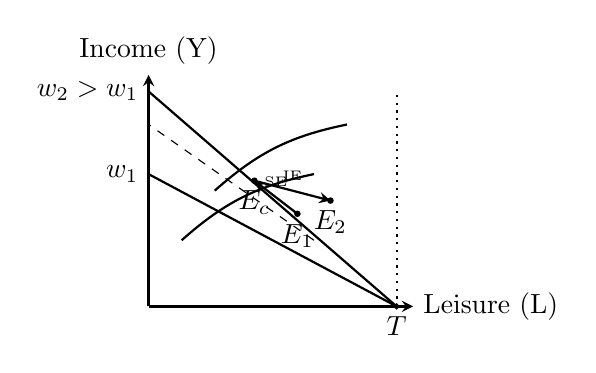
\begin{tikzpicture}[scale=0.42, thick, >=stealth]
    \draw[->] (0,0) -- (8,0) node[right] {Leisure (L)};
    \draw[->] (0,0) -- (0,7) node[above] {Income (Y)};
    % Time endowment
    \filldraw (7.5,0) circle (1.5pt) node[below] {$T$};
    \draw[dotted] (7.5,0) -- (7.5,6.5);
    % Budget lines
    \draw (7.5,0) -- (0,4) node[left] {$w_1$};
    \draw (7.5,0) -- (0,6.5) node[left] {$w_2 > w_1$};
    % Compensated BL (dashed)
    \draw[dashed, thin] (5,2) -- (0,5.5);
    % Indifference curves
    \draw (5,4) to[bend right=15] (1,2);
    \draw (6,5.5) to[bend right=15] (2,3.5);
    \filldraw (4.5,2.8) circle (1.8pt) node[below] {$E_1$};
    \filldraw (3.2,3.8) circle (1.8pt) node[below] {$E_c$};
    \filldraw (5.5,3.2) circle (1.8pt) node[below] {$E_2$};
    \draw[->] (4.5,2.8) -- (3.2,3.8) node[midway, above] {\tiny SE};
    \draw[->] (3.2,3.8) -- (5.5,3.2) node[midway, above] {\tiny IE};
\end{tikzpicture}
\end{center}

\textbf{Analysis:}
\begin{itemize}[leftmargin=*,nosep]
    \item \textbf{Substitution Effect (SE):} A higher wage makes leisure more expensive (higher opportunity cost). The consumer substitutes \textit{away} from leisure toward work (more income). $L \downarrow$, $H \uparrow$. SE is always positive for work.
    \item \textbf{Income Effect (IE):} A higher wage increases real income. If leisure is a \textbf{normal good}, the consumer ``buys'' more leisure (works less). $L \uparrow$, $H \downarrow$. IE is negative for work.
    \item \textbf{Net Effect:} Depends on relative magnitudes.
    \begin{itemize}[nosep]
        \item \textbf{At low wages:} SE dominates $\to$ wage increase $\to$ more work ($H \uparrow$). Labor supply curve slopes upward.
        \item \textbf{At high wages:} IE may dominate $\to$ wage increase $\to$ less work ($H \downarrow$). Labor supply curve bends backward.
    \end{itemize}
\end{itemize}

\textbf{Empirical Evidence:}
\begin{itemize}[leftmargin=*,nosep]
    \item Male labor supply is relatively inelastic; the backward bend is observed at very high income levels (e.g., professionals reducing hours, early retirement).
    \item Female labor supply elasticity is higher; participation decisions dominate.
    \item Over the 20th century, wages rose dramatically, yet average weekly hours fell (from 60+ to ~40), consistent with a dominant long-run income effect.
    \item Recent studies of ride-share drivers (Uber, Lyft) show strong evidence of income targeting behavior -- drivers work less when hourly earnings are high, indicating a strong income effect (reference-dependent preferences).
\end{itemize}

\textbf{Policy Implications:}
\begin{enumerate}[leftmargin=*,nosep]
    \item \textbf{Taxation and Labor Supply:} A tax cut raises the after-tax wage. Whether it increases labor supply depends on the relative strength of SE and IE. The Laffer curve concept depends partly on this.
    \item \textbf{Overtime Pay:} Premium overtime wages (1.5x, 2x) have both SE (more incentive to work extra hours) and IE (higher overall income), making the net effect on total hours ambiguous.
    \item \textbf{Welfare Programs:} Design of welfare/transfer programs (Earned Income Tax Credit -- EITC) must consider labor supply responses. EITC increases effective wages for low-income workers (SE dominant) while providing income support, encouraging work.
\end{enumerate}

\textbf{Economic Lesson:} The work-leisure model demonstrates the power of indifference curve analysis in decomposing complex behavioral responses to economic incentives, with profound implications for tax and welfare policy.

% ============================================================================
% PART 9: EXAM QUESTIONS
% ============================================================================
\section*{9. Exam Questions \& Model Answers}

\subsection*{Question 1: Properties and Proof}
\textbf{Prove that two indifference curves cannot intersect.}

\textbf{Answer:} Assume two indifference curves $IC_1$ and $IC_2$ intersect at point $A$. Since $A$ is on both curves, the consumer is indifferent between $A$ and any other point on $IC_1$, and also between $A$ and any point on $IC_2$. Choose point $B$ on $IC_1$ and point $C$ on $IC_2$ such that $C$ has more of both goods than $B$. Since $A$ is on $IC_1$, consumer is indifferent between $A$ and $B$. Since $A$ is on $IC_2$, consumer is indifferent between $A$ and $C$. By transitivity, consumer must be indifferent between $B$ and $C$. But $C$ has more of both goods than $B$; by non-satiation, $C$ is strictly preferred to $B$. Contradiction. Therefore, indifference curves cannot intersect.

\vspace{0.2cm}

\subsection*{Question 2: Equilibrium and Comparative Statics}
\textbf{A consumer has $U = x^{0.5} y^{0.5}$. $P_x = 2$, $P_y = 4$, $M = 120$.}
\textbf{(a) Find optimal bundle.}
\textbf{(b) If $P_x$ falls to \$1, find new equilibrium and decompose total effect using Hicksian method.}
\textbf{(c) Derive the demand function for $x$ and the equation of the Price Consumption Curve.}

\vspace{0.1cm}
\textbf{Solution:}
\textbf{(a)} $MU_x = 0.5 x^{-0.5} y^{0.5}$, $MU_y = 0.5 x^{0.5} y^{-0.5}$.
$MRS = MU_x/MU_y = y/x$. At equilibrium: $y/x = 2/4 = 1/2 \Rightarrow y = 0.5x$.
Budget: $2x + 4(0.5x) = 120 \Rightarrow 2x + 2x = 120 \Rightarrow 4x = 120 \Rightarrow \mathbf{x=30, y=15}$.

\textbf{(b)} New $P_x = 1$. MRS = $P_x/P_y \Rightarrow y/x = 1/4 \Rightarrow y = 0.25x$.
Budget: $1x + 4(0.25x) = 120 \Rightarrow x + x = 120 \Rightarrow 2x=120 \Rightarrow \mathbf{x=60, y=15}$.
\textit{Total Effect:} $\Delta x = 60 - 30 = +30$.

\textit{SE (Hicks):} Find utility at $E_1$: $U = 30^{0.5} \cdot 15^{0.5} = \sqrt{450} \approx 21.21$. Find bundle at new prices ($P_x=1, P_y=4$) that gives this $U$ at minimum cost: $y/x = 0.25 \Rightarrow y=0.25x$. $U = x^{0.5}(0.25x)^{0.5} = x^{0.5} \cdot 0.5 x^{0.5} = 0.5x = 21.21 \Rightarrow x_c = 42.42$.
$SE = 42.42 - 30 = +12.42$ (increase in $x$ due to relative price change only).
$IE = 60 - 42.42 = +17.58$ (increase in $x$ because real income rose).
Since $IE > 0$, $x$ is a normal good (and a luxury here since spending on $x$ remains constant at \$60).

\textbf{(c)} Demand for $x$ (from MRS condition $y/x = P_x/P_y \Rightarrow P_x x = P_y y$): Income is spent equally. $P_x x = M/2$. Demand: $\mathbf{x = M/(2P_x)}$. PCC equation: $y = (P_x/P_y) x$, but $P_x x = M/2$, so $y = M/(2P_y)$ constant. PCC is a \textbf{horizontal line} at $y = M/(2P_y)$ (both goods normal, and in Cobb-Douglas with equal exponents, expenditure on $y$ is fixed when $M$ constant but $P_x$ changes). More generally, the PCC is the locus of points satisfying $y/x = P_x/P_y$ with $P_x x + P_y y = M$ as $P_x$ varies. Here it simplifies.

\vspace{0.2cm}

\subsection*{Question 3: Conceptual}
\textbf{Using indifference curve analysis, explain why the demand curve for a normal good must slope downwards.}

\textbf{Answer:} Consider a fall in $P_x$:
\begin{itemize}[leftmargin=*,nosep]
    \item \textbf{Substitution Effect:} The relative price of $x$ falls. Holding real income constant, the consumer substitutes toward $x$ and away from $y$. $x$ increases. This effect is always negative (price falls $\to$ quantity rises).
    \item \textbf{Income Effect:} The price fall increases real income. For a \textbf{normal good}, higher real income leads to an increase in consumption. So $x$ increases further.
\end{itemize}
Both effects work in the same direction: $x$ unambiguously rises when $P_x$ falls. Therefore, the demand curve (plotting $P_x$ against $x$) must be \textbf{downward sloping}. There is no theoretical possibility of an upward-sloping demand curve for a normal good. The Giffen paradox can only arise for strongly inferior goods where the negative income effect (less $x$ as real income rises) outweighs the substitution effect.

\vspace{0.2cm}

\subsection*{Question 4: Application}
\textbf{A government subsidizes the price of a staple food for low-income households. Using indifference curve analysis, compare this price subsidy to an equivalent-value cash transfer. Which policy places the consumer on a higher indifference curve? Why might the government still choose the price subsidy?}

\textbf{Answer:} A price subsidy rotates the budget line outward specifically for the subsidized good (change in relative prices). A cash transfer shifts the budget line outward parallelly. For the same government cost, the cash transfer generally places the consumer on a \textbf{higher indifference curve} because it imposes no restriction on consumption choices (the consumer can always choose the same bundle as under the subsidy, but may prefer a different one). The price subsidy introduces a distortion: it artificially lowers the relative price, encouraging overconsumption of the subsidized good relative to the consumer's true preferences ($MRS \neq P_x/P_y$ at the equilibrium without further adjustment by the consumer).

\textbf{However}, governments may prefer price subsidies due to:
\begin{itemize}[nosep]
    \item \textbf{Paternalism:} Ensuring the good consumed is nutritious food rather than potentially harmful alternatives.
    \item \textbf{Externalities:} If consumption of the good has positive externalities (e.g., healthier children $\to$ lower public health costs), the price subsidy can correct an underconsumption problem.
    \item \textbf{Political acceptability:} Taxpayers may be more willing to fund food subsidies than unrestricted cash.
    \item \textbf{Intra-household allocation:} Cash may be captured by certain household members and not benefit children; in-kind transfers may target intended beneficiaries better.
\end{itemize}

\end{multicols}

% ============================================================================
% SUMMARY TABLE
% ============================================================================
\vspace{0.3cm}
\begin{center}
\fbox{\begin{minipage}{0.9\textwidth}
\footnotesize
\textbf{Summary Cheat Sheet: Indifference Curve Analysis}
\begin{center}
\begin{tabular}{@{}p{3.2cm}p{2.8cm}p{3.2cm}@{}}
\toprule
\textbf{Concept} & \textbf{Key Formula/Condition} & \textbf{Significance} \\
\midrule
Indifference Curve & $U(x,y) = \text{const}$ & Bundles yielding equal satisfaction \\
MRS & $MU_x / MU_y$ & Slope of IC; willingness to trade \\
Budget Line & $P_x x + P_y y = M$ & Affordable bundles; slope $= -P_x/P_y$ \\
Consumer Equilibrium & $MRS = P_x/P_y$ & Tangency of IC and BL \\
Income Consumption Curve & Locus of equilibria as $M$ varies & Basis for Engel curve \\
Price Consumption Curve & Locus of equilibria as $P_x$ varies & Basis for demand curve \\
Substitution Effect & Movement along original IC to new price ratio & Always non-positive for own price \\
Income Effect & Movement to new IC (shift) & Sign depends on good type \\
Total Effect & $TE = SE + IE$ & Decomposes price effect \\
\bottomrule
\end{tabular}
\end{center}

\vspace{0.1cm}
\textbf{Quick Reference: Effects of $P_x \downarrow$}
\begin{itemize}[leftmargin=*,nosep]
    \item Normal Good: SE $+$ and IE $+$ $\to$ unambiguous $x \uparrow$, Demand slopes down.
    \item Inferior (non-Giffen): SE $+$, IE $-$ but $|SE| > |IE|$ $\to$ $x \uparrow$, Demand slopes down.
    \item Giffen Good: SE $+$, IE $-$ and $|IE| > |SE|$ $\to$ $x \downarrow$, Demand slopes up (rare).
\end{itemize}
\end{minipage}}
\end{center}

\end{document}
\newpage

% ============================================================================
% TOPIC 6: Production and Cost
% ============================================================================
\documentclass[10pt,a4paper]{article}
\usepackage[margin=0.7in]{geometry}
\usepackage{multicol}
\usepackage{amsmath}
\usepackage{tikz}
\usepackage{enumitem}
\usepackage{titlesec}
\usepackage{booktabs}
\usepackage{fontspec}

% Compact formatting
\setlength{\columnsep}{0.7cm}
\setlength{\parindent}{0pt}
\setlength{\parskip}{0.12cm}
\titlespacing{\section}{0pt}{0.4cm}{0.15cm}
\titlespacing{\subsection}{0pt}{0.25cm}{0.08cm}
\titlespacing{\subsubsection}{0pt}{0.2cm}{0.05cm}

% Custom section style
\titleformat{\section}{\large\bfseries}{}{0em}{}
\titleformat{\subsection}{\normalsize\bfseries}{}{0em}{}
\titleformat{\subsubsection}{\normalsize\bfseries\itshape}{}{0em}{}

\begin{document}

\begin{center}
{\LARGE \textbf{Production and Cost}}\\[0.15cm]
{\normalsize \textit{Topic 6: Theory of the Firm -- Output, Inputs, and Cost Curves}}\\[0.15cm]
\hrule
\end{center}
\vspace{-0.3cm}

\begin{multicols}{2}
\footnotesize

% ============================================================================
% PART 1: DEFINITIONS AND CORE CONCEPTS
% ============================================================================
\section*{1. Core Definitions}

\subsection*{Production Function}
A \textbf{Production Function} expresses the \textbf{technological relationship} between physical inputs (factors of production) and the maximum physical output obtainable, given the current state of technology.

\[
Q = f(L, K, N, E, \dots)
\]
Where: $Q$ = Total product/output; $L$ = Labor; $K$ = Capital; $N$ = Land/Natural resources; $E$ = Entrepreneurship.

\textbf{Key Properties:}
\begin{itemize}[leftmargin=*,nosep]
    \item \textbf{Technical Efficiency:} Gives \textit{maximum} output for given inputs (no waste).
    \item \textbf{Flow Concept:} Output is measured per unit of time.
    \item \textbf{Technology-Specific:} A change in technology shifts the function.
    \item \textbf{Specifies Factor Proportions:} How inputs combine (complements vs. substitutes).
\end{itemize}

\subsection*{Factors of Production: Fixed vs. Variable}
The distinction is based on the \textbf{time horizon}:
\begin{itemize}[leftmargin=*,nosep]
    \item \textbf{Fixed Factors:} Cannot be changed in the \textbf{short run} (e.g., factory building, heavy machinery, land). Their quantity remains constant regardless of output level.
    \item \textbf{Variable Factors:} Can be adjusted in the short run (e.g., labor, raw materials, electricity). Their quantity varies directly with output.
    \item \textbf{Short Run:} At least one factor is fixed. The firm operates within a given ``scale'' of plant. $Q = f(L, \bar{K})$.
    \item \textbf{Long Run:} All factors are variable. The firm can change its scale of operations. No fixed factors. $Q = f(L, K)$ -- both variable.
\end{itemize}

% ============================================================================
% PART 2: HOW TO REMEMBER
% ============================================================================
\section*{2. Memory Triggers and Conceptual Anchors}

\begin{itemize}[leftmargin=*,nosep]
    \item \textbf{Production Function = Recipe:} Inputs (ingredients) $\to$ Output (cake). Technology = cooking method. Better tech = more cake from same ingredients.
    \item \textbf{Fixed vs Variable = ``Can I change it this month?'':} Fixed = ``Stuck with it'' (lease, building). Variable = ``I can hire/fire or buy more'' (workers, materials). Mnemonic: \textbf{S}hort run = \textbf{S}tuck with some factors.
    \item \textbf{Total Product (TP) = Total Output.} Marginal Product (MP) = \textbf{Extra} output from \textbf{one more} unit of variable input. (M for Marginal = More input.)
    \item \textbf{MP and AP Relationship:}
    \begin{itemize}[nosep]
        \item If $MP > AP$, AP is \textbf{rising} (a high marginal student raises the class average).
        \item If $MP < AP$, AP is \textbf{falling} (a low marginal student lowers the average).
        \item $MP$ intersects $AP$ at the \textbf{maximum} of $AP$.
    \end{itemize}
    \item \textbf{Law of Diminishing Returns = Too Many Cooks in the Kitchen:} Adding more and more workers to a fixed kitchen increases total meals initially, but eventually each extra worker adds less (and may even reduce output). Mnemonic: ``Crowding kills productivity.''
    \item \textbf{Returns to Scale = Double the Recipe:}
    \begin{itemize}[nosep]
        \item Double all inputs, output \textbf{more than doubles} = \textbf{Increasing Returns to Scale (IRS)}. (Bulk buying, specialization.)
        \item Double all inputs, output \textbf{exactly doubles} = \textbf{Constant Returns to Scale (CRS)}.
        \item Double all inputs, output \textbf{less than doubles} = \textbf{Decreasing Returns to Scale (DRS)}. (Management complexity.)
    \end{itemize}
    \item \textbf{Cost Curves -- Shape Memory:}
    \begin{itemize}[nosep]
        \item \textbf{TC} starts positive (due to fixed cost) and rises.
        \item \textbf{MC, AVC, ATC} are \textbf{U-shaped}: First fall due to specialization/returns, then rise due to diminishing returns.
        \item \textbf{AFC} always falls (spreading overhead over more units).
        \item \textbf{MC} cuts \textbf{AVC} and \textbf{ATC} at their \textbf{minimum points}. (If marginal is below average, average falls; if above, average rises.)
    \end{itemize}
    \item \textbf{Short Run vs. Long Run Cost:} LR cost curve is the \textbf{envelope} of SR cost curves. In the LR, you can choose the optimal plant size for each output level.
\end{itemize}

% ============================================================================
% PART 3: MATHEMATICAL FRAMEWORK
% ============================================================================
\section*{3. Product Concepts \& Formulas}

\subsection*{Total, Average, and Marginal Product}
Let $Q = f(L, \bar{K})$ be the short-run production function with Labor ($L$) as the variable factor.

\textbf{Total Product of Labor ($TP_L$):} $TP_L = Q = f(L, \bar{K})$.

\textbf{Average Product of Labor ($AP_L$):}
\[
AP_L = \frac{TP_L}{L} = \frac{Q}{L}
\]
Measures output per unit of labor (productivity).

\textbf{Marginal Product of Labor ($MP_L$):}
\[
MP_L = \frac{\Delta TP_L}{\Delta L} \quad \text{or} \quad MP_L = \frac{\partial Q}{\partial L}
\]
Additional output from one more unit of labor.

\subsection*{The Law of Diminishing Marginal Returns (Diminishing MP)}
As more units of a \textbf{variable input} are added to a \textbf{fixed input}, eventually the \textbf{marginal product} of the variable input \textbf{declines}, \textit{ceteris paribus}.
\[
\frac{\partial (MP_L)}{\partial L} = \frac{\partial^2 Q}{\partial L^2} < 0 \quad \text{(after some point)}
\]

\textbf{Three Stages of Production (Short-Run):}
\begin{enumerate}[leftmargin=*,nosep]
    \item \textbf{Stage I ($AP_L$ rising):} $MP_L > AP_L$. Increasing average returns. Fixed factors underutilized. \textit{Rational producer won't stop here} (can increase AP by adding more L).
    \item \textbf{Stage II ($AP_L$ falling, $MP_L > 0$):} $MP_L < AP_L$, but $MP_L > 0$. TP still rising. \textbf{This is the rational production range.}
    \item \textbf{Stage III ($MP_L < 0$):} Total product falls. Too many workers relative to fixed capital; negative returns. \textit{Irrational to operate here.}
\end{enumerate}

\subsection*{Returns to Scale (Long-Run Concept)}
When \textbf{all} inputs increase by the same proportion $\lambda > 1$, how does output change?
\[
Q = f(L, K) \quad \Rightarrow \quad \text{Measure } f(\lambda L, \lambda K)
\]
\begin{itemize}[leftmargin=*,nosep]
    \item \textbf{Increasing Returns to Scale (IRS):} $f(\lambda L, \lambda K) > \lambda f(L, K)$ $\Rightarrow$ Output increases more than proportionately.
    \item \textbf{Constant Returns to Scale (CRS):} $f(\lambda L, \lambda K) = \lambda f(L, K)$ $\Rightarrow$ Output increases exactly proportionately. Function is \textbf{homogeneous of degree 1}.
    \item \textbf{Decreasing Returns to Scale (DRS):} $f(\lambda L, \lambda K) < \lambda f(L, K)$ $\Rightarrow$ Output increases less than proportionately.
\end{itemize}

\textbf{Typical Production Function (Cobb-Douglas):}
\[
Q = A L^\alpha K^\beta
\]
Returns to scale: $\alpha + \beta$.
\begin{itemize}[nosep]
    \item $\alpha + \beta > 1 \Rightarrow$ IRS.
    \item $\alpha + \beta = 1 \Rightarrow$ CRS.
    \item $\alpha + \beta < 1 \Rightarrow$ DRS.
\end{itemize}

\textbf{Causes:} IRS due to specialization, indivisibilities, dimensional factors. DRS due to management complexity, coordination problems (``diseconomies of scale'').

\subsection*{Cost Concepts \& Formulas}
\textbf{Total Costs:}
\[
TC = TFC + TVC
\]
\begin{itemize}[nosep]
    \item \textbf{Total Fixed Cost (TFC):} Cost of fixed factors; does not vary with output. (e.g., rent, insurance).
    \item \textbf{Total Variable Cost (TVC):} Cost of variable factors; varies directly with output. (e.g., wages, raw material). $TVC = w \cdot L(Q)$.
\end{itemize}

\textbf{Average Costs:}
\[
AFC = \frac{TFC}{Q}; \quad AVC = \frac{TVC}{Q}; \quad ATC = \frac{TC}{Q} = AFC + AVC
\]

\textbf{Marginal Cost ($MC$):}
\[
MC = \frac{\Delta TC}{\Delta Q} = \frac{\Delta TVC}{\Delta Q} \quad \text{(since TFC constant)}
\]
\[
MC = \frac{w}{MP_L} \quad \text{(Derived: } MC = \frac{d(TVC)}{dQ} = \frac{w \cdot dL}{dQ} = \frac{w}{MP_L}\text{)}
\]
\textbf{Inverse relationship:} When $MP_L$ is rising, $MC$ is falling; when $MP_L$ falls (diminishing returns), $MC$ rises. The U-shape of MC mirrors the inverted-U of MP.

\subsection*{Short-Run vs. Long-Run Cost Curves}
\begin{itemize}[leftmargin=*,nosep]
    \item \textbf{Short-Run Average Cost (SRAC):} U-shaped due to fixed factor constraint; diminishing returns eventually raise AVC and ATC.
    \item \textbf{Long-Run Average Cost (LRAC):} \textbf{Envelope curve} of all possible SRAC curves (each SRAC corresponds to a different plant size). LRAC is typically U-shaped due to economies/diseconomies of scale.
    \item In LR, all factors variable; firm chooses optimal plant size for each output level. LRAC touches each SRAC at the minimum-cost point for that output level (tangency, not necessarily minimum of each SRAC).
\end{itemize}

% ============================================================================
% PART 4: GRAPHICAL ANALYSIS
% ============================================================================
\section*{4. Graphical Illustrations}

\subsection*{TP, AP, and MP Curves \& Stages of Production}
\begin{center}
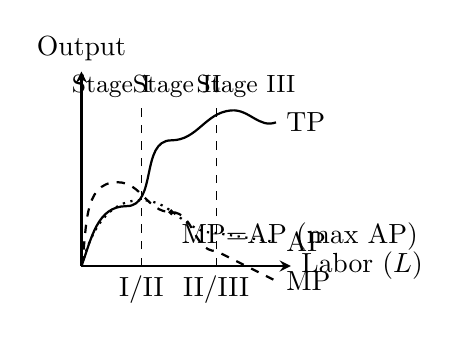
\begin{tikzpicture}[scale=0.38, thick, >=stealth]
    \draw[->] (0,0) -- (7,0) node[right] {Labor ($L$)};
    \draw[->] (0,0) -- (0,6.5) node[above] {Output};
    % TP Curve (sigmoid)
    \draw[thick] (0,0) to[out=70,in=180] (1.5,2) to[out=0,in=180] (3,4.2) to[out=0,in=185] (5,5.2) to[out=5,in=200] (6.5,4.8) node[right] {TP};
    % MP Curve
    \draw[thick, dashed] (0,0) to[out=80,in=180] (1.2,2.8) to[out=0,in=180] (3,1.8) to[out=0,in=180] (4.5,0.5) -- (6.5,-0.5) node[right] {MP};
    % AP Curve
    \draw[thick, dotted] (0,0) to[out=75,in=180] (2,2.2) to[out=0,in=180] (4.5,1.1) -- (6.5,0.8) node[right] {AP};
    % Stage divisions
    \draw[dashed, thin] (2,0) node[below] {I/II} -- (2,5.5);
    \draw[dashed, thin] (4.5,0) node[below] {II/III} -- (4.5,5.5);
    \node at (1,6) {\small Stage I};
    \node at (3.2,6) {\small Stage II};
    \node at (5.5,6) {\small Stage III};
    % MP=AP intersection
    \filldraw (3,1.8) circle (1.5pt) node[below right] {MP=AP (max AP)};
\end{tikzpicture}
\end{center}

\subsection*{Short-Run Cost Curves (Family of Curves)}
\begin{center}
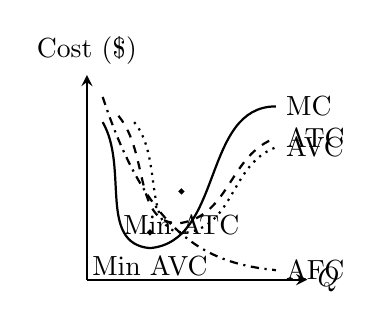
\begin{tikzpicture}[scale=0.4, thick, >=stealth]
    \draw[->] (0,0) -- (7,0) node[right] {$Q$};
    \draw[->] (0,0) -- (0,6.5) node[above] {Cost (\$)};
    % MC
    \draw[thick] (0.5,5) to[out=300,in=175] (2,1) to[out=5,in=180] (6,5.5) node[right] {MC};
    % ATC
    \draw[thick, dashed] (1,5.2) to[out=310,in=185] (3,1.8) to[out=10,in=200] (6,4.5) node[right] {ATC};
    % AVC
    \draw[thick, dotted] (1.5,5) to[out=310,in=185] (3.2,1.5) to[out=10,in=200] (6,4.2) node[right] {AVC};
    % AFC
    \draw[thick, dashdotted] (0.5,5.8) .. controls (2,1.2) and (4,0.5) .. (6,0.3) node[right] {AFC};
    % Intersection points
    \filldraw (2,1.5) circle (1.5pt) node[below=5pt] {Min AVC};
    \filldraw (3,2.8) circle (1.5pt) node[below=5pt] {Min ATC};
\end{tikzpicture}
\end{center}
\textit{Note: MC intersects AVC and ATC at their respective minimum points. ATC = AVC + AFC. The vertical gap between ATC and AVC shrinks as AFC declines.}

\subsection*{Long-Run Average Cost (LRAC) as Envelope}
\begin{center}
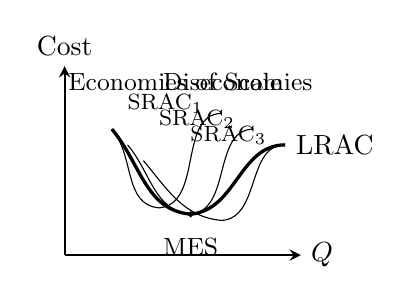
\begin{tikzpicture}[scale=0.4, thick, >=stealth]
    \draw[->] (0,0) -- (7.5,0) node[right] {$Q$};
    \draw[->] (0,0) -- (0,6) node[above] {Cost};
    % SRAC curves
    \draw[thin] (1.5,4) to[out=310,in=175] (3,1.5) to[out=5,in=180] (5,4.5);
    \draw[thin] (2,3.5) to[out=310,in=175] (4,1.3) to[out=5,in=180] (6,4);
    \draw[thin] (2.5,3) to[out=310,in=175] (5,1.1) to[out=5,in=180] (7,3.5);
    \node at (3.2,4.8) {\footnotesize SRAC$_1$}; \node at (4.2,4.3) {\footnotesize SRAC$_2$}; \node at (5.2,3.8) {\footnotesize SRAC$_3$};
    % LRAC envelope
    \draw[very thick] (1.5,4) to[out=310,in=175] (4,1.3) to[out=5,in=180] (7,3.5) node[right] {LRAC};
    \node at (3.5,5.5) {\small Economies of Scale};
    \node at (5.5,5.5) {\small Diseconomies};
    \filldraw (4,1.3) circle (1.5pt) node[below=5pt] {\small MES};
\end{tikzpicture}
\end{center}
\textit{LRAC is the lower envelope of all SRAC curves. Minimum Efficient Scale (MES) is the lowest output level at which LRAC is minimized.}

\columnbreak

% ============================================================================
% PART 5: DETAILED RELATIONSHIPS
% ============================================================================
\section*{5. Key Relationships and Derivations}

\subsection*{Product-Cost Duality}
There is a \textbf{mathematical duality} between production and cost:
\begin{itemize}[leftmargin=*,nosep]
    \item \textbf{MC and MP:} $MC = \frac{w}{MP_L}$. When MP is high (Stage I), MC is low. When diminishing returns set in (MP falls, Stage II), MC rises.
    \item \textbf{AVC and AP:} $AVC = \frac{w \cdot L}{Q} = \frac{w}{AP_L}$. When AP is high, AVC is low. AVC falls when AP rises, and rises when AP falls. AVC reaches minimum at maximum AP.
    \item \textbf{Shape connection:} The U-shape of MC and AVC is derived directly from the inverted-U shape of MP and AP, respectively.
\end{itemize}

\subsection*{Why MC Intersects AVC and ATC at Minimum}
\textbf{Mathematical Proof:} At the minimum of AVC, $\frac{d(AVC)}{dQ} = 0$.
\[
AVC = \frac{TVC}{Q} \quad \Rightarrow \quad \frac{d(AVC)}{dQ} = \frac{Q \cdot \frac{d(TVC)}{dQ} - TVC \cdot 1}{Q^2} = \frac{Q \cdot MC - TVC}{Q^2}
\]
Setting derivative = 0: $Q \cdot MC = TVC \Rightarrow MC = \frac{TVC}{Q} = AVC$.

Similarly, at min ATC: $MC = ATC$. This is \textbf{essential for cost-curve diagram accuracy}.

\subsection*{Long-Run Cost Minimization}
In the long run, the firm chooses $L$ and $K$ to minimize cost for a given output $\bar{Q}$:
\[
\min \; wL + rK \quad \text{s.t.} \quad f(L, K) = \bar{Q}
\]
Condition: $MRTS_{LK} = \frac{MP_L}{MP_K} = \frac{w}{r}$.
Cost function: $C(Q) = wL^*(w,r,Q) + rK^*(w,r,Q)$.

\subsection*{Economies and Diseconomies of Scale}
\begin{itemize}[leftmargin=*,nosep]
    \item \textbf{Economies of Scale (falling LRAC):} Caused by \textbf{specialization of labor/management}, \textbf{indivisibilities} of capital (large machines more efficient), \textbf{volume discounts} on inputs, \textbf{learning by doing}, \textbf{by-product utilization}.
    \item \textbf{Diseconomies of Scale (rising LRAC):} Caused by \textbf{management complexity}, \textbf{communication breakdowns}, \textbf{alienation of labor}, \textbf{increased bureaucracy}, \textbf{transportation costs} as the firm grows geographically.
    \item \textbf{Constant Returns to Scale (flat LRAC):} Perfect scalability; firm can replicate operations efficiently.
\end{itemize}

% ============================================================================
% PART 6: EXTENSIVE CASE STUDIES
% ============================================================================
\section*{6. Comprehensive Case Studies}

\subsection*{Case Study 1: Henry Ford's Assembly Line and the Law of Diminishing Returns}

\textbf{Background:} In 1913, Henry Ford revolutionized automobile manufacturing by introducing the \textbf{moving assembly line} at the Highland Park plant in Michigan. Prior to this, cars were handcrafted by skilled workers. The assembly line broke production into specialized, repetitive tasks, dramatically increasing productivity and reducing costs. The Model T price fell from \$850 (1908) to under \$300 (1924), making the automobile a mass-market product.

\textbf{Production Function Analysis:}
\begin{itemize}[leftmargin=*,nosep]
    \item \textbf{Short-run:} Capital (assembly line, factory) was fixed. Labor was variable.
    \item \textbf{Initial phase (Stage I and early Stage II):} Adding workers to the fixed assembly line led to \textbf{increasing marginal returns}. With specialization, workers became faster at their single repeated task. The division of labor raised $MP_L$. Total product rose sharply, and $AP_L$ (output per worker) increased.
    \item \textbf{Optimal point:} Ford's $5-a-day wage policy (double the prevailing wage) reduced turnover and absenteeism, keeping the labor force stable and productive. The plant operated near the boundary of Stage I and Stage II, where $MP_L \approx AP_L$, maximizing labor productivity.
\end{itemize}

\textbf{The Diminishing Returns Test:}
In later years, Ford attempted to push the system further by continuously speeding up the assembly line and adding more workers to the same physical plant. At some point, diminishing returns set in:
\begin{itemize}[leftmargin=*,nosep]
    \item Workers became \textbf{overcrowded} on the line; task spaces were physically constrained.
    \item Fatigue increased; error rates and accidents rose.
    \item The marginal product of an additional worker became very low; too many workers per machine caused idle time and interference.
    \item Total product still grew, but at a diminishing rate (Stage II). Eventually, adding more workers could have led to negative marginal product (Stage III) -- workers literally getting in each other's way.
\end{itemize}

\textbf{Cost Implications:}
\begin{itemize}[leftmargin=*,nosep]
    \item Initially, high $MP_L$ meant low $MC$ ($MC = w/MP_L$). The \$5 wage was easily absorbed by the massive productivity gains.
    \item As diminishing returns set in, $MP_L$ fell, and $MC$ began to rise. AVC also started increasing after the point of maximum AP.
    \item Ford eventually had to build entirely new, larger plants (e.g., River Rouge Complex, completed 1928) because the existing fixed capital (Highland Park) constrained further output expansion. This was the \textbf{transition from Short Run to Long Run} -- scaling up all inputs to escape the constraints of the fixed factor.
\end{itemize}

\textbf{The River Rouge Complex -- Economies of Scale (Long-Run):}
The River Rouge plant was the largest integrated factory in the world. It demonstrated massive \textbf{internal economies of scale}:
\begin{itemize}[leftmargin=*,nosep]
    \item \textbf{Vertical Integration:} Raw materials (iron ore, coal) arrived at one end; finished Model A cars drove out the other end.
    \item \textbf{Technical Economies:} Specialized machinery for each component (engine blocks, chassis, glass), achieving very low unit costs.
    \item \textbf{Labor Specialization:} Over 100,000 workers, each highly specialized.
    \item \textbf{By-product Use:} Slag from steel production was sold; waste heat reused.
\end{itemize}
However, as the plant grew even larger, \textbf{diseconomies of scale} emerged:
\begin{itemize}[leftmargin=*,nosep]
    \item Management coordination became extremely complex; bureaucratic layers multiplied.
    \item Labor relations deteriorated; the massive workforce was difficult to manage, leading to the famous 1937 ``Battle of the Overpass'' union clashes.
    \item Communication and scheduling across the huge site became inefficient.
    \item LRAC likely began to rise at very large output scales.
\end{itemize}

\textbf{Economic Lessons:}
\begin{enumerate}[leftmargin=*,nosep]
    \item The \textbf{short-run production function} with diminishing returns explains both early productivity miracles and eventual constraints within a given plant.
    \item The \textbf{transition from SR to LR} is a strategic decision: when diminishing returns make MC rise too high, the firm expands fixed capital.
    \item \textbf{Economies of scale} drive long-run cost reductions, but \textbf{diseconomies of scale} eventually limit firm size. Ford's trajectory illustrates both sides of the U-shaped LRAC curve.
    \item The relationship $MC = w/MP_L$ directly links worker productivity to marginal cost -- the fundamental driver of pricing and profitability.
\end{enumerate}

\subsection*{Case Study 2: Semiconductor Fabrication -- Returns to Scale and the Cost Race (TSMC vs. Intel)}

\textbf{Background:} Semiconductor manufacturing (chip fabrication, or ``fabs'') is one of the most capital-intensive industries in the world. A single state-of-the-art fabrication plant costs \$10--\$20 billion. The industry is characterized by massive \textbf{economies of scale}, a steep \textbf{learning curve}, and intense competition driven by cost-per-transistor reduction. Taiwan Semiconductor Manufacturing Company (TSMC) has become the world's dominant player by focusing solely on manufacturing (a ``pure-play foundry''), while Intel historically combined design and manufacturing (IDM model).

\textbf{Production Function:}
The output of a fab can be modeled as a function of capital-intensive equipment (lithography machines, etchers) and highly skilled labor.
\[
Q = f(K, L) \quad \text{with significant fixed capital } K \text{ (ASML EUV machines cost \$200M+ each)}
\]

\textbf{Short-Run Production:}
\begin{itemize}[leftmargin=*,nosep]
    \item \textbf{Fixed Factor:} The fab building and installed equipment ($K$ fixed). Expanding output requires running the fab at higher capacity utilization rates, adding shifts, overtime ($L$ variable).
    \item \textbf{Initially:} MP of labor may rise as the workforce gets trained and processes are optimized (learning-by-doing within a shift).
    \item \textbf{Eventually:} Diminishing returns hit. Adding extra shifts (nights, weekends) leads to worker fatigue, increased defect rates, equipment downtime, and maintenance constraints. The marginal wafer output from an extra labor hour declines. Running fabs above 90--95\% capacity utilization becomes inefficient ($MC$ rises sharply due to defects and breakdowns).
\end{itemize}

\textbf{Long-Run Returns to Scale:}
When Intel or TSMC build a new fab (increasing $K$ and $L$ proportionately), they experience significant economies of scale:

\begin{enumerate}[leftmargin=*,nosep]
    \item \textbf{Technical Indivisibilities:} An EUV lithography machine produces wafers at a massive minimum scale. A larger fab better utilizes the high fixed cost of these machines. \textbf{Doubling fab size more than doubles output} because the most expensive tools operate more efficiently.
    \item \textbf{Learning and Experience Curve:} Cumulative output drives down defect densities and improves yield (the percentage of functional chips per wafer). TSMC's cumulative output is enormous, giving it a cost advantage Intel struggles to match. \textit{Yield improvement} is a pure economy of scale -- fixed R\&D and learning costs spread over larger volume.
    \item \textbf{Economies of Scope:} Advanced fabs can produce multiple chip designs for different clients, sharing the massive fixed costs across many products. TSMC's pure-play model amplifies this -- it serves hundreds of clients (Apple, AMD, Nvidia) on the same process technology.
    \item \textbf{R\&D Amortization:} Semiconductor process R\&D costs billions per node (e.g., moving from 7nm to 5nm technology). These costs are fixed regardless of how many chips are eventually produced. TSMC's large volume allows it to amortize R\&D across a far greater number of chips than Intel, lowering \textbf{average fixed cost (AFC)} dramatically.
\end{enumerate}

\textbf{The Cost Race -- Why Size Matters:}
The average cost per transistor has fallen exponentially (Moore's Law), but the cost per fab has risen exponentially (Rock's Law). This creates a \textbf{virtuous cycle} of scale for the leader:
\begin{itemize}[leftmargin=*,nosep]
    \item Larger volume $\to$ lower AFC and ATC $\to$ lower prices $\to$ more customers $\to$ even larger volume.
    \item TSMC's market share in advanced logic chips exceeds 90\%. Intel, despite its history, has struggled to achieve the scale to compete on cost.
\end{itemize}

\textbf{Diseconomies of Scale -- The Risk for TSMC:}
\begin{itemize}[leftmargin=*,nosep]
    \item \textbf{Geopolitical Concentration:} TSMC's dominance creates supply chain risk (Taiwan Strait tensions). The US CHIPS Act (2022, \$52B subsidies) aims to diversify production.
    \item \textbf{Complexity Management:} As TSMC grows, managing dozens of simultaneous processes, thousands of clients, and supply chains across the globe introduces coordination costs. Some analysts point to potential diseconomies: bureaucratic delays, difficulty in quality control across numerous fabs in different countries.
    \item \textbf{Water and Energy Constraints:} Fabs consume enormous amounts of ultrapure water and electricity. In Taiwan (and Arizona, for TSMC's expansions), resource scarcity imposes \textbf{external diseconomies} that raise costs.
\end{itemize}

\textbf{Graphical Representation of Cost Dynamics:}
\begin{center}
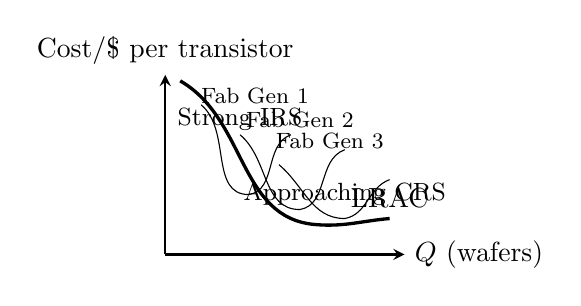
\begin{tikzpicture}[scale=0.38, thick, >=stealth]
    \draw[->] (0,0) -- (8,0) node[right] {$Q$ (wafers)};
    \draw[->] (0,0) -- (0,6) node[above] {Cost/\$ per transistor};
    % LRAC curve: steeply falling, then flat
    \draw[very thick] (0.5,5.8) to[out=330,in=175] (5,1) to[out=355,in=185] (7.5,1.2) node[above] {LRAC};
    \node at (2.5,4.5) {\small Strong IRS};
    \node at (6,2) {\small Approaching CRS};
    % SRAC curves
    \draw[thin] (1.2,5) to[out=320,in=180] (2.8,2) to[out=10,in=200] (4.2,4);
    \draw[thin] (2.5,4) to[out=320,in=180] (4.5,1.5) to[out=10,in=200] (6,3.5);
    \draw[thin] (3.8,3) to[out=320,in=180] (6,1.2) to[out=10,in=200] (7.5,2.5);
    \node at (3,5.3) {\footnotesize Fab Gen 1};
    \node at (4.5,4.5) {\footnotesize Fab Gen 2};
    \node at (5.5,3.8) {\footnotesize Fab Gen 3};
\end{tikzpicture}
\end{center}
\textit{Each SRAC represents a generation of fab technology. LRAC is the envelope, falling steeply then flattening as diminishing returns to scale (managerial complexity) offset technical economies.}

\textbf{Economic Lessons:}
\begin{enumerate}[leftmargin=*,nosep]
    \item \textbf{Returns to scale} are the central competitive dynamic in capital-intensive industries. The firm with larger scale has lower ATC and can underprice rivals.
    \item \textbf{Learning curves} and fixed R\&D amortization are critical sources of increasing returns to scale.
    \item \textbf{The SR vs. LR distinction:} Short-run capacity constraints (diminishing returns within a fab) create business cycle dynamics (chip shortages). Long-run expansion (new fabs) involves strategic scale decisions.
    \item Government industrial policy (CHIPS Act) recognizes the public-good and national-security externality of having domestic scale in semiconductor production, given massive economies of scale.
\end{enumerate}

% ============================================================================
% PART 7: EXAM QUESTIONS
% ============================================================================
\section*{7. Exam Practice Questions \& Model Answers}

\subsection*{Question 1: Calculating Products and Costs}
\textbf{Firm's production function: $Q = 2L^{0.5}$, where $Q$ is output and $L$ is labor. Wage rate $w = \$20$.}
\textbf{(a) Derive $TP_L$, $AP_L$, and $MP_L$ for $L = 1, 4, 9, 16$.}
\textbf{(b) At what $L$ does diminishing returns set in?}
\textbf{(c) Find $TVC$, $AVC$, and $MC$ as functions of $Q$.}
\textbf{(d) Show that $MC = w / MP_L$.}

\vspace{0.1cm}
\textbf{Solution:}
\vspace{0.05cm}
\textbf{(a)}
\begin{tabular}{@{}c|c|c|c@{}}
\hline $L$ & $Q = 2L^{0.5}$ & $AP_L = Q/L$ & $MP_L = dQ/dL = L^{-0.5}$ \\
\hline 1 & 2.00 & 2.00 & 1.00 \\
4 & 4.00 & 1.00 & 0.50 \\
9 & 6.00 & 0.67 & 0.33 \\
16 & 8.00 & 0.50 & 0.25 \\
\hline
\end{tabular}

\textbf{(b)} $MP_L = L^{-0.5}$. $d(MP_L)/dL = -0.5 L^{-1.5} < 0$ for all $L>0$. \textbf{Diminishing returns set in immediately} from the first unit of labor. (This function has diminishing MP throughout.)

\textbf{(c)} $Q = 2L^{0.5} \Rightarrow L = Q^2/4$. $TVC = wL = 20 \cdot (Q^2/4) = 5Q^2$.
$AVC = TVC/Q = 5Q$. $MC = d(TVC)/dQ = 10Q$.

\textbf{(d)} $MP_L = L^{-0.5} = (Q^2/4)^{-0.5} = 2/Q$. $w/MP_L = 20 / (2/Q) = 10Q = MC$. Verified. $\checkmark$

\vspace{0.2cm}

\subsection*{Question 2: Short-Run and Long-Run Costs}
\textbf{A firm's production is $Q = \sqrt{LK}$. In the short run, $K = 16$. $w = 4$, $r = 1$.}
\textbf{(a) Derive SR cost functions: TC(Q), ATC(Q), MC(Q).}
\textbf{(b) In the long run, find the cost-minimizing $L$ and $K$ for a given $Q$, and the LR cost function $C(Q)$.}
\textbf{(c) Compare SR and LR ATC for $Q = 4$, $Q = 8$, $Q = 16$. Explain differences.}

\vspace{0.05cm}
\textbf{Solution:}
\vspace{0.05cm}
\textbf{(a)} SR: $K=16$. $Q = \sqrt{L \cdot 16} = 4\sqrt{L} \Rightarrow L = Q^2/16$.
$TC = wL + rK = 4(Q^2/16) + 1(16) = Q^2/4 + 16$.
$ATC = Q/4 + 16/Q$. $MC = Q/2$.

\textbf{(b)} LR: $MRTS = MP_L/MP_K = \frac{0.5 K^{0.5} L^{-0.5}}{0.5 L^{0.5} K^{-0.5}} = K/L$. Set $K/L = w/r = 4 \Rightarrow K = 4L$.
Output: $Q = \sqrt{L \cdot 4L} = \sqrt{4L^2} = 2L \Rightarrow L = Q/2$, $K = 4(Q/2) = 2Q$.
$C(Q) = 4(Q/2) + 1(2Q) = 2Q + 2Q = 4Q$.
$LRAC = 4$, $LRMC = 4$ (constant returns to scale).

\textbf{(c)}
\begin{itemize}[nosep]
    \item $Q=4$: SR ATC = $4/4 + 16/4 = 1+4 = 5$. LR AC = $4$. SR cost higher (overcapitalized).
    \item $Q=8$: SR ATC = $8/4 + 16/8 = 2+2 = 4$. LR AC = $4$. SR = LR (\textbf{tangency point}: $K=16$ is optimal for $Q=8$).
    \item $Q=16$: SR ATC = $16/4 + 16/16 = 4+1 = 5$. LR AC = $4$. SR cost higher (undercapitalized for larger $Q$).
\end{itemize}

\vspace{0.2cm}

\subsection*{Question 3: Conceptual Comparison}
\textbf{Distinguish clearly between the ``Law of Diminishing Returns'' and ``Decreasing Returns to Scale.'' Provide real-world examples.}

\vspace{0.05cm}
\textbf{Answer:}
\begin{center}
\begin{tabular}{@{}p{2.8cm}p{3cm}p{3cm}@{}}
\toprule
\textbf{Feature} & \textbf{Diminishing Returns} & \textbf{Decreasing Returns to Scale} \\
\midrule
Time Horizon & \textbf{Short Run} (at least one fixed factor) & \textbf{Long Run} (all factors variable) \\
Cause & Adding variable input to fixed input $\to$ congestion & Increasing all inputs proportionately $\to$ output rises less than proportionately \\
Reason & Overcrowding, inefficiency with fixed capacity & Management complexity, coordination problems, bureaucracy \\
Example & Adding more workers to a fixed-size office reduces per-worker output & A startup that grows into a multinational faces communication breakdowns and slower growth \\
\bottomrule
\end{tabular}
\end{center}
\textit{Analogy:} Diminishing returns is like adding more chefs to a fixed kitchen; decreasing returns to scale is like trying to run a global restaurant chain and struggling with management.

\vspace{0.2cm}

\subsection*{Question 4: Application/Graphical}
\textbf{Draw and explain the relationship between MP, AP, MC, and AVC curves. Why does MC intersect AVC at the minimum of AVC?}

\vspace{0.05cm}
\textbf{Answer:} (Provide description and graph). The relationship stems from the duality $AVC = w/AP_L$ and $MC = w/MP_L$. When $AP_L$ is maximum, $AVC$ is minimum. When $MP_L = AP_L$ (intersection at max AP), $MC = AVC$ (intersection at min AVC). The ``average-marginal relationship'' in mathematics dictates: if the marginal is below the average, the average falls; if above, it rises. Thus, $MC$ must equal $AVC$ exactly at the minimum point of $AVC$. The same logic applies for $ATC$.

\end{multicols}

% ============================================================================
% SUMMARY TABLE
% ============================================================================
\vspace{0.3cm}
\begin{center}
\fbox{\begin{minipage}{0.9\textwidth}
\footnotesize
\textbf{Summary Cheat Sheet: Production and Cost}
\begin{center}
\begin{tabular}{@{}p{3cm}p{2.8cm}p{3.2cm}@{}}
\toprule
\textbf{Concept} & \textbf{Formula} & \textbf{Key Insight} \\
\midrule
Production Function & $Q = f(L, K)$ & Maximum output from given inputs \\
Marginal Product & $MP_L = \partial Q/\partial L$ & Extra output from one more unit of labor \\
Average Product & $AP_L = Q/L$ & Output per worker; productivity \\
Diminishing Returns (SR) & $\partial MP_L/\partial L < 0$ & Variable factor on fixed factor $\to$ MP eventually falls \\
Returns to Scale (LR) & $f(\lambda L, \lambda K) \text{ vs. } \lambda Q$ & IRS/CRS/DRS depending on proportional output response \\
$TC = TFC + TVC$ & Sum of fixed and variable costs & TFC independent of Q; TVC rises with Q \\
$MC = dTC/dQ$ & $= w/MP_L$ & Inverse of MP; U-shaped \\
$ATC = AFC + AVC$ & $= TC/Q$ & U-shaped; envelope of AVC and AFC \\
$MC$ cuts $AVC$, $ATC$ & At their minimum points & Mathematical necessity: marginal pulls average \\
LRAC & Envelope of SRACs & Firm chooses optimal plant size for each Q \\
\bottomrule
\end{tabular}
\end{center}

\vspace{0.1cm}
\textbf{Quick Check: Cost Curve Shapes and Causes}
\begin{itemize}[leftmargin=*,nosep]
    \item \textbf{U-shape of MC:} Initially falls due to specialization/returns; rises due to diminishing returns.
    \item \textbf{U-shape of AVC/ATC:} Driven by MC. MC below $\to$ AVC falls; MC above $\to$ AVC rises.
    \item \textbf{AFC falls continuously:} ``Spreading overhead'' -- TFC divided by increasing Q.
    \item \textbf{LRAC U-shape:} Economies of scale (falling), then diseconomies (rising).
\end{itemize}
\end{minipage}}
\end{center}

\end{document}
\newpage

% ============================================================================
% TOPIC 7: Firm Decisions, Revenue and Market Structure
% ============================================================================
\documentclass[10pt,a4paper]{article}
\usepackage[margin=0.7in]{geometry}
\usepackage{multicol}
\usepackage{amsmath}
\usepackage{tikz}
\usepackage{enumitem}
\usepackage{titlesec}
\usepackage{booktabs}
\usepackage{fontspec}

% Compact formatting
\setlength{\columnsep}{0.7cm}
\setlength{\parindent}{0pt}
\setlength{\parskip}{0.12cm}
\titlespacing{\section}{0pt}{0.4cm}{0.15cm}
\titlespacing{\subsection}{0pt}{0.25cm}{0.08cm}
\titlespacing{\subsubsection}{0pt}{0.2cm}{0.05cm}

% Custom section style
\titleformat{\section}{\large\bfseries}{}{0em}{}
\titleformat{\subsection}{\normalsize\bfseries}{}{0em}{}
\titleformat{\subsubsection}{\normalsize\bfseries\itshape}{}{0em}{}

\begin{document}

\begin{center}
{\LARGE \textbf{Firm Decisions, Revenue \& Market Structure}}\\[0.15cm]
{\normalsize \textit{Topic 7: Optimal Input Choice, Profit Maximization, and Market Power}}\\[0.15cm]
\hrule
\end{center}
\vspace{-0.3cm}

\begin{multicols}{2}
\footnotesize

% ============================================================================
% PART 1: DEFINITIONS AND CORE CONCEPTS
% ============================================================================
\section*{1. Core Definitions}

\subsection*{Isoquants and Isocosts}
\textbf{Isoquant:} An \textbf{isoquant} (Equal-Quantity curve) shows all combinations of two inputs (typically Labor $L$ and Capital $K$) that produce the \textbf{same level of output}. It is the firm's analog of the consumer's indifference curve.
\[
Q = f(L, K) = \bar{Q} \quad \text{(constant)}
\]

\textbf{Isocost Line:} An \textbf{isocost} (Equal-Cost line) shows all combinations of $L$ and $K$ that cost the firm the \textbf{same total expenditure}.
\[
C = wL + rK \quad \Rightarrow \quad K = \frac{C}{r} - \frac{w}{r}L
\]
Where: $w$ = wage rate, $r$ = rental rate of capital. Slope of isocost = $-w/r$ (relative input price ratio).

\subsection*{Least Cost Combination (Optimal Input Choice)}
The firm minimizes cost for a given output level by choosing $L$ and $K$ where the isoquant is \textbf{tangent} to the lowest possible isocost line:
\[
MRTS_{LK} = \frac{MP_L}{MP_K} = \frac{w}{r}
\]
\textbf{Marginal Rate of Technical Substitution (MRTS):} The rate at which the firm can substitute $L$ for $K$ while keeping output constant. It equals the ratio of marginal products. At optimum, the last dollar spent on each input yields the same additional output.

\subsection*{Revenue Concepts}
\begin{itemize}[leftmargin=*,nosep]
    \item \textbf{Total Revenue (TR):} $TR = P \times Q$.
    \item \textbf{Average Revenue (AR):} $AR = TR/Q = P$. The demand curve \textbf{is} the AR curve.
    \item \textbf{Marginal Revenue (MR):} $MR = \Delta TR / \Delta Q = d(TR)/dQ$. Additional revenue from selling one more unit.
\end{itemize}

\textbf{Relationship between AR and MR:}
\begin{itemize}[leftmargin=*,nosep]
    \item \textbf{Perfect Competition:} Firm is a price-taker. $P$ is constant. $AR = MR = P$ (horizontal demand curve).
    \item \textbf{Imperfect Competition (Monopoly, Monopolistic Competition, Oligopoly):} Firm faces downward-sloping demand. To sell more, price must fall on \textbf{all} units. $MR < AR = P$. $MR$ curve lies below the demand (AR) curve.
    \[
    MR = P \left(1 + \frac{1}{E_d}\right) \quad \text{or} \quad MR = P \left(1 - \frac{1}{|E_d|}\right)
    \]
    Since $E_d < 0$, $MR < P$ for downward-sloping demand.
\end{itemize}

% ============================================================================
% PART 2: HOW TO REMEMBER
% ============================================================================
\section*{2. Memory Triggers and Conceptual Anchors}

\begin{itemize}[leftmargin=*,nosep]
    \item \textbf{Isoquant = Same Quantity = Production IC:} Just like indifference curves, but for output. Higher isoquant = more output.
    \item \textbf{Isocost = Same Cost = Budget Line:} Just like the consumer's budget line, but for the firm. Slope $= -w/r$ (relative price of labor).
    \item \textbf{Least Cost Tangency:} $MRTS = w/r$. The rate at which you \textit{can} trade machines for workers in the market (price ratio) equals the rate at which you \textit{need} to trade them to keep output constant (MP ratio). ``The market trade-off matches the technical trade-off.''
    \item \textbf{MR vs AR in Imaginary Markets:}
    \begin{itemize}[nosep]
        \item \textbf{Perfect Competition:} ``I can sell all I want at the market price.'' $MR = P$. AR curve is a flat line.
        \item \textbf{Monopoly:} ``To sell more, I must lower the price on EVERY unit.'' $MR$ is below $P$, steeper than demand. ``Price cut bleeds revenue from inframarginal units.''
    \end{itemize}
    \item \textbf{Profit Max Rule:} $MR = MC$. If $MR > MC$: produce more (adds more to revenue than cost). If $MR < MC$: produce less. At $MR = MC$, profit is maximized. \textbf{This rule is universal across ALL market structures.}
    \item \textbf{Market Structure Spectrum -- ``Many to One'':}
    \begin{itemize}[nosep]
        \item \textbf{Perfect Competition:} Infinite firms, identical product.
        \item \textbf{Monopolistic Competition:} Many firms, differentiated product.
        \item \textbf{Oligopoly:} Few firms, strategic interaction.
        \item \textbf{Monopoly:} One firm, no close substitutes.
    \end{itemize}
    \item \textbf{Game Theory in Oligopoly:} ``Prisoner's Dilemma'' -- both firms could earn higher profits by cooperating (high prices), but each has an incentive to cheat (lower price), leading to a worse joint outcome.
\end{itemize}

% ============================================================================
% PART 3: MATHEMATICAL FRAMEWORK
% ============================================================================
\section*{3. Mathematical Formulation}

\subsection*{Cost Minimization Problem}
\[
\min_{L, K} \; wL + rK \quad \text{s.t.} \quad f(L, K) = Q_0
\]
Lagrangian: $\mathcal{L} = wL + rK + \lambda (Q_0 - f(L, K))$.
First-order conditions:
\[
w - \lambda \frac{\partial f}{\partial L} = 0; \quad r - \lambda \frac{\partial f}{\partial K} = 0; \quad Q_0 = f(L, K)
\]
Dividing: $\frac{w}{r} = \frac{MP_L}{MP_K} = MRTS_{LK}$.

The solution $L^*(w, r, Q_0)$, $K^*(w, r, Q_0)$ are \textbf{conditional factor demands}. The cost function $C(w, r, Q_0) = wL^* + rK^*$.

\subsection*{Revenue Functions and MR}
For linear demand $P = a - bQ$:
\[
TR = P \cdot Q = aQ - bQ^2
\]
\[
AR = \frac{TR}{Q} = a - bQ = P
\]
\[
MR = \frac{d(TR)}{dQ} = a - 2bQ
\]
Note: $MR$ has twice the slope of the demand curve ($-2b$ vs. $-b$). Both share same vertical intercept ($a$ on the price axis).

\textbf{MR in terms of elasticity:}
\[
MR = \frac{d(TR)}{dQ} = P + Q \cdot \frac{dP}{dQ} = P \left(1 + \frac{Q}{P} \cdot \frac{dP}{dQ}\right) = P\left(1 + \frac{1}{E_d}\right)
\]

\subsection*{Profit Maximization Condition}
\[
\pi(Q) = TR(Q) - TC(Q)
\]
First-order condition: $\frac{d\pi}{dQ} = MR - MC = 0 \Rightarrow \mathbf{MR = MC}$.
Second-order condition: $\frac{d^2\pi}{dQ^2} < 0 \Rightarrow \frac{d(MR)}{dQ} < \frac{d(MC)}{dQ}$ (slope of MR < slope of MC at optimum).

\textbf{Market-Specific MR:}
\begin{itemize}[nosep]
    \item \textbf{Perfect Competition:} $P$ constant, $MR = P$. Thus condition: $P = MC$.
    \item \textbf{Monopoly:} $MR = P(1 + 1/E_d) = MC$. Since $E_d < 0$, $P > MC$. Markup: $\frac{P - MC}{P} = \frac{1}{|E_d|}$ (Lerner Index).
\end{itemize}

\subsection*{Market Structures Summary Equations}
\begin{center}
\begin{tabular}{@{}p{2cm}p{1.8cm}p{2.2cm}@{}}
\toprule
\textbf{Structure} & \textbf{Demand} & \textbf{Profit Max} \\
\midrule
Perfect Comp. & $P = AR = MR$ (flat) & $P = MC$ ($Q$ where $P=MC$) \\
Monopoly & $P > MR$ (downward) & $MR = MC$, then $P > MC$ \\
Monop. Comp. & $P > MR$ (downward) & $MR = MC$ (SR profit, LR break-even) \\
Oligopoly & Downward (\& interdependent) & $MR = MC$ given rivals' strategies \\
\bottomrule
\end{tabular}
\end{center}

% ============================================================================
% PART 4: GRAPHICAL ANALYSIS
% ============================================================================
\section*{4. Graphical Illustrations}

\subsection*{Isocost-Isoquant: Least Cost Combination}
\begin{center}
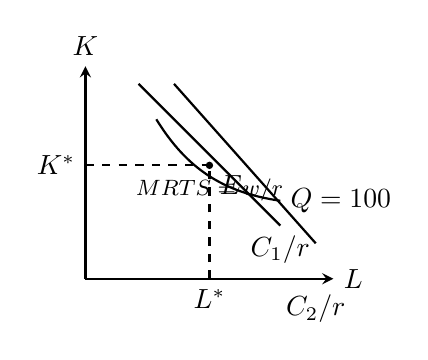
\begin{tikzpicture}[scale=0.45, thick, >=stealth]
    \draw[->] (0,0) -- (7,0) node[right] {$L$};
    \draw[->] (0,0) -- (0,6) node[above] {$K$};
    % Isocost lines
    \draw[thick] (1.5,5.5) -- (5.5,1.5) node[below] {$C_1 / r$};
    \draw[thick] (2.5,5.5) -- (6.5,1) node[below=15pt] {$C_2 / r$};
    % Isoquant
    \draw[thick] (2,4.5) to[bend right=25] (5.5,2.2) node[right] {$Q=100$};
    % Tangency point
    \filldraw (3.5,3.2) circle (2pt) node[below right] {$E$};
    \node at (3.5,2.5) {\footnotesize $MRTS = w/r$};
    \draw[dashed] (3.5,0) node[below] {$L^*$} -- (3.5,3.2);
    \draw[dashed] (0,3.2) node[left] {$K^*$} -- (3.5,3.2);
\end{tikzpicture}
\end{center}
\textit{Point $E$ minimizes cost for producing $Q=100$. The firm cannot afford the $C_2$ isocost; $C_1$ is affordable but produces less than 100. At E, $MRTS = w/r$.}

\subsection*{MR and AR for a Monopolist (Linear Demand)}
\begin{center}
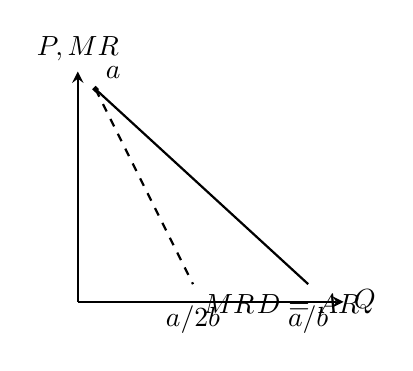
\begin{tikzpicture}[scale=0.45, thick, >=stealth]
    \draw[->] (0,0) -- (7.5,0) node[right] {$Q$};
    \draw[->] (0,0) -- (0,6.5) node[above] {$P, MR$};
    % Demand (AR) curve
    \draw[thick] (0.5,6) -- (6.5,0.5) node[below] {$D = AR$};
    % MR curve (twice the slope)
    \draw[thick, dashed] (0.5,6) -- (3.25,0.5) node[below right] {$MR$};
    \filldraw (0.5,6) circle (1.5pt) node[above right] {$a$};
    \node at (3.25,-0.5) {$a/2b$}; \node at (6.5,-0.5) {$a/b$};
\end{tikzpicture}
\end{center}
\textit{For $P = a - bQ$, $MR = a - 2bQ$. MR is twice as steep and crosses the x-axis at half the quantity.}

\subsection*{Profit Maximization: MR = MC}
\begin{center}
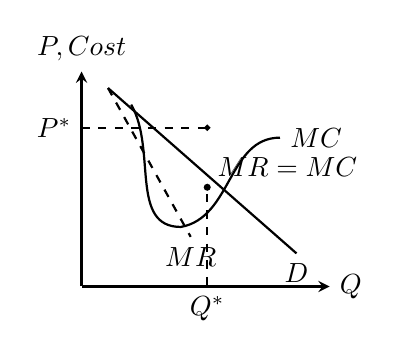
\begin{tikzpicture}[scale=0.42, thick, >=stealth]
    \draw[->] (0,0) -- (7.5,0) node[right] {$Q$};
    \draw[->] (0,0) -- (0,6.5) node[above] {$P, Cost$};
    \draw[thick] (0.8,6) -- (6.5,1) node[below] {$D$};
    \draw[thick, dashed] (0.8,6) -- (3.3,1.5) node[below] {$MR$};
    \draw[thick] (1.5,5.5) to[out=300, in=180] (3,1.8) to[out=10, in=180] (6,4.5) node[right] {$MC$};
    \filldraw (3.8,3) circle (2pt) node[above right] {$MR=MC$};
    \draw[dashed] (3.8,2.8) -- (3.8,0) node[below] {$Q^*$};
    \draw[dashed] (0,4.8) node[left] {$P^*$} -- (3.8,4.8);
    \filldraw (3.8,4.8) circle (1.5pt);
\end{tikzpicture}
\end{center}
\textit{Firm produces $Q^*$ where $MR=MC$. Price $P^*$ is read from the demand curve at $Q^*$. Shaded area (if ATC was drawn) = profit.}

% ============================================================================
% PART 5: MARKET STRUCTURES - DETAILED ANALYSIS
% ============================================================================
\section*{5. Market Structure Models (Detailed)}

\subsection*{Perfect Competition}
\textbf{Characteristics:}
\begin{itemize}[leftmargin=*,nosep]
    \item \textbf{Large number} of buyers and sellers -- no single agent affects price.
    \item \textbf{Homogeneous} product -- perfect substitutes.
    \item \textbf{Free entry and exit} -- zero barriers.
    \item \textbf{Perfect information} -- all agents know prices and technology.
    \item Firm is a \textbf{price taker}.
\end{itemize}

\textbf{Short-Run Equilibrium:} $P = MC$. Firm may earn \textbf{supernormal profit} ($P > ATC$), \textbf{normal profit} ($P = ATC$), or operate at \textbf{loss} ($P < ATC$ but $P > AVC$) to minimize loss. Shutdown if $P < AVC$.

\textbf{Long-Run Equilibrium:} Free entry/exit drives economic profit to zero. $P = MC = \min ATC$. \textbf{Allocative efficiency} ($P = MC$) and \textbf{productive efficiency} ($P = \min ATC$) achieved.

\subsection*{Monopoly}
\textbf{Characteristics:}
\begin{itemize}[leftmargin=*,nosep]
    \item \textbf{Single seller}, no close substitutes.
    \item \textbf{High barriers to entry} (legal, patents, control of resources, natural monopoly).
    \item Firm is a \textbf{price maker}, faces market demand.
\end{itemize}

\textbf{Equilibrium:} $MR = MC$, then charge $P^*$ from demand curve. $P^* > MC$. \textbf{Deadweight loss} exists (underproduction relative to competitive ideal).

\textbf{Price Discrimination:} Monopolist can increase profit by charging different prices to different consumers:
\begin{itemize}[nosep]
    \item 1st Degree (Perfect): Each consumer pays their maximum willingness to pay. No consumer surplus remains.
    \item 2nd Degree: Different prices for different quantities (bulk discounts, block pricing).
    \item 3rd Degree: Different prices in different market segments based on elasticity (e.g., student/senior discounts).
\end{itemize}

\subsection*{Monopolistic Competition (Chamberlin)}
\textbf{Characteristics:}
\begin{itemize}[leftmargin=*,nosep]
    \item \textbf{Many sellers}, free entry/exit.
    \item \textbf{Differentiated products} -- perceived or real quality differences, branding, location. Each firm has slight market power.
    \item Demand curve is \textbf{highly elastic} but downward-sloping.
\end{itemize}

\textbf{Short-Run:} Like a mini-monopoly. $MR = MC$, earns profit/loss.

\textbf{Long-Run:} Entry drives profit to zero ($P = ATC$). But unlike perfect competition, $P > MC$ (not allocatively efficient) and $P > \min ATC$ (excess capacity -- firm produces left of minimum efficient scale). Consumers pay higher price but enjoy \textbf{variety}.

\subsection*{Oligopoly and Game Theory}
\textbf{Characteristics:}
\begin{itemize}[leftmargin=*,nosep]
    \item \textbf{Few dominant firms}; high barriers to entry.
    \item Products may be homogeneous (steel, oil) or differentiated (automobiles, smartphones).
    \item \textbf{Strategic interdependence} -- each firm's decisions depend on rivals' expected actions. Modeled using \textbf{Game Theory}.
\end{itemize}

\textbf{Cournot Model (Quantity Competition):} Firms choose output simultaneously. Each firm's optimal output depends on rival's output. Equilibrium: each correctly guesses the other's output; no incentive to deviate. Market price between competitive and monopoly levels.

\textbf{Bertrand Model (Price Competition):} Firms set prices simultaneously. With homogeneous goods, undercutting drives price down to $MC$ (paradoxically, two firms can yield competitive outcome).

\textbf{Game Theory -- Prisoner's Dilemma (Oligopoly Pricing):}
Two firms (A and B) decide: \textbf{High Price (Cooperate)} or \textbf{Low Price (Defect)}.
\begin{center}
\begin{tabular}{cc|c|c|}
\multicolumn{2}{c}{} & \multicolumn{2}{c}{\textbf{Firm B}} \\
\multicolumn{2}{c}{} & High Price & Low Price \\
\cline{3-4}
\multirow{2}{*}{\textbf{Firm A}} & High Price & (10, 10) & (2, 15) \\
\cline{3-4}
& Low Price & (15, 2) & (5, 5) \\
\cline{3-4}
\end{tabular}
\end{center}
\textit{(Payoffs in millions. A's payoff first, B's second.)}
\begin{itemize}[nosep]
    \item \textbf{Dominant Strategy for Each:} Low Price (Defect). Regardless of rival's choice, defecting yields higher payoff.
    \item \textbf{Nash Equilibrium:} (Low, Low) $\to$ (5, 5).
    \item \textbf{Cooperative Outcome:} (High, High) $\to$ (10, 10) is better for both but unstable because each has incentive to cheat.
    \item This explains why cartels (like OPEC) tend to break down without enforcement.
\end{itemize}

\textbf{Collusion and Cartels:} Firms may collude (jointly set $MR = MC$, act like a monopoly) to maximize joint profits. Illegal in most jurisdictions (antitrust laws). Cartels face incentive to cheat (prisoner's dilemma) and must have enforcement mechanisms.

\textbf{Kinked Demand Curve (Sweezy Model):} Explains price rigidity in oligopoly. Competitors match price cuts but not price increases. Creates a kink in the demand curve and a discontinuous MR curve; MC can shift within the gap without changing optimal price.

% ============================================================================
% PART 6: EXTENSIVE CASE STUDIES
% ============================================================================
\section*{6. Comprehensive Case Studies}

\subsection*{Case Study 1: OPEC and the Prisoner's Dilemma of Oil Cartels (1973--2024)}

\textbf{Background:} The Organization of the Petroleum Exporting Countries (OPEC), formed in 1960, is the world's most famous (and only partially successful) cartel. It controls roughly 40\% of global oil production. OPEC's core dilemma is the classic \textbf{prisoner's dilemma}: all members collectively benefit from restricting output to keep prices high, but each member individually benefits from cheating and producing more than its quota.

\textbf{Cooperative Equilibrium (Cartel Profit Maximization):}
OPEC acts as a \textbf{multi-plant monopolist}. It sets total output where $MR_{\text{world oil}} = MC_{\text{aggregate}}$ and allocates quotas to members. The collective monopoly price ($P_m$) is high; each member earns supernormal profits.

\textbf{Incentive to Cheat:}
Each member country faces an individual $P > MC$ (since P is set at monopoly level). If a single country (e.g., Saudi Arabia in some periods, Iraq, Venezuela) secretly increases production above its quota, it sells more barrels at the high monopoly price, increasing its own revenue. The price effect (small price drop from extra output) is borne by \textit{all} members, while the quantity effect (extra revenue) accrues to the cheater alone. This is the \textbf{free-rider problem} in cartels.

\textbf{Historical Evidence: Prisoner's Dilemma in Action.}

\textit{Episode 1: 1973 Oil Embargo \& 1970s Success.} OPEC successfully cut production, quadrupling prices. Members initially cooperated. The high price held because demand was highly inelastic in the short run.

\textit{Episode 2: 1980s Collapse.} As high prices persisted, demand became more elastic (conservation, fuel-efficient cars). Non-OPEC supply expanded (North Sea, Alaska). OPEC members, facing reduced market share, began \textbf{cheating on quotas}. Saudi Arabia, traditionally the ``swing producer,'' cut its output to defend prices alone, but other members overproduced. By 1986, oil prices crashed from \$30 to below \$10/barrel. The cartel had collapsed into the non-cooperative Nash equilibrium (high output, low price).

\textit{Episode 3: 2020 Price War (Saudi Arabia vs. Russia).} After COVID-19 crushed demand, OPEC+ (OPEC plus Russia) attempted to coordinate production cuts. Russia refused to cut its quota. Saudi Arabia responded by flooding the market (a strategic play in the repeated game), driving prices negative briefly (WTI futures hit -\$37). This was a \textbf{punishment strategy} in a repeated game: Saudi Arabia signaled its willingness to endure short-term pain to enforce long-term cooperation. The cartel subsequently agreed to historic production cuts.

\textit{Episode 4: 2022--2024 Coordination Amid Geopolitical Tension.} The Russia-Ukraine war disrupted supply. OPEC+ maintained cuts, demonstrating that when external shocks align members' interests (everyone gains from high prices with limited ability to expand output), cooperation can hold. However, internal tensions (smaller African producers wanting to produce more, UAE seeking higher baseline quotas) persist.

\textbf{Game Theory Lessons:}
\begin{enumerate}[leftmargin=*,nosep]
    \item \textbf{Static game (one-shot):} Defection (cheating) is the dominant strategy $\to$ cartel unstable.
    \item \textbf{Repeated game:} If the game is infinitely repeated, \textbf{tit-for-tat} strategies (cooperate if rival cooperated last period; defect if they defected) can sustain cooperation if the discount rate is low enough (future profits matter). Saudi Arabia has often played this role.
    \item \textbf{Monitoring and Punishment:} Effective cartels need transparency (observing output) and enforcement mechanisms. OPEC's monitoring has been historically weak, leading to endemic cheating.
    \item \textbf{Market Structure evolves:} Entry of new producers (shale oil, renewables) erodes cartel power. The shale revolution made non-OPEC supply more elastic, limiting OPEC's ability to raise prices without losing significant market share.
\end{enumerate}

\textbf{Economic Concepts Demonstrated:} Prisoner's dilemma, dominant strategy, Nash equilibrium, cartel instability, repeated game strategies, elasticity and monopoly power.

\subsection*{Case Study 2: The Streaming Wars -- Oligopoly and Strategic Interaction (Netflix, Disney+, Amazon Prime, 2019--2024)}

\textbf{Background:} The global streaming video market evolved from a near-monopoly (Netflix, 2015--2019) to an \textbf{oligopoly} with the entry of deep-pocketed competitors: Disney+ (2019), Apple TV+ (2019), HBO Max (2020, now Max), Amazon Prime Video, and others. The industry exemplifies non-price competition, strategic investment, and game-theoretic behavior.

\textbf{Market Structure Analysis:}
\begin{itemize}[leftmargin=*,nosep]
    \item \textbf{Few major firms (Oligopoly):} Netflix, Disney+, Amazon Prime, Max, Apple TV+ dominate. High concentration but no single monopoly.
    \item \textbf{High barriers to entry:} Massive content spending (billions annually for original programming), technology infrastructure, and subscriber base lock-in. New entrants need enormous capital.
    \item \textbf{Differentiated products:} Each platform differentiates by exclusive content (Netflix: \textit{Stranger Things}; Disney+: Marvel, Star Wars; Amazon: \textit{LOTR: Rings of Power}; Apple: \textit{Ted Lasso}).
    \item \textbf{Strategic interdependence:} Pricing, content spending, and bundling decisions are made with rivals' expected reactions in mind.
\end{itemize}

\textbf{Game Theory: A Content Spending ``Arms Race''}

The competition resembles a \textbf{prisoner's dilemma} in content investment.

\textit{Scenario:} Two firms (Netflix and Disney+) must choose: \textbf{High Content Budget (\$15B+)} or \textbf{Moderate Content Budget (\$8B)}.

\begin{center}
\begin{tabular}{cc|c|c|}
\multicolumn{2}{c}{} & \multicolumn{2}{c}{\textbf{Disney+}} \\
\multicolumn{2}{c}{} & High Budget & Moderate Budget \\
\cline{3-4}
\multirow{2}{*}{\textbf{Netflix}} & High Budget & (5, 4) & (9, 2) \\
\cline{3-4}
& Moderate Budget & (2, 9) & (7, 7) \\
\cline{3-4}
\end{tabular}
\end{center}
\textit{(Hypothetical profit indices. High spending $\to$ high subscriber appeal but high costs.)}

\begin{itemize}[leftmargin=*,nosep]
    \item If both choose \textbf{Moderate Budget}, they earn reasonable profits (7, 7). Total industry profitability is high.
    \item However, if one spends \textbf{High} while the other spends Moderate, the high-spender captures market share and subscriber growth (9 vs. 2 for the rival).
    \item \textbf{Dominant Strategy?} If each fears the rival will spend high, the best response is also to spend high (to avoid being left behind). The Nash Equilibrium is (High, High) with profits (5, 4) -- lower for both than (Moderate, Moderate).
    \item This is precisely what happened: Netflix, Disney, Amazon, and Apple all ramped up content spending to \$10--\$20 billion per year, eroding profitability. Netflix's free cash flow was negative for years due to this arms race.
\end{itemize}

\textbf{Strategic Behavior Observed:}
\begin{enumerate}[leftmargin=*,nosep]
    \item \textbf{Non-Price Competition:} Price competition is muted (prices crept up slowly). Primary competition is through \textbf{content quality/exclusivity} (differentiation) and \textbf{marketing}. This is classic monopolistic competition / oligopoly behavior -- avoid price wars, compete on non-price dimensions.
    \item \textbf{Entry Deterrence / Pre-emption:} Netflix's massive early spending on originals was partly a \textbf{first-mover strategy} to build a content library so large that rivals would find it difficult to compete (barrier to entry).
    \item \textbf{Bundling (Economies of Scope):} Disney+ bundled with Hulu and ESPN+; Amazon Prime Video bundled with Prime shipping; Apple TV+ bundled with Apple One. Bundling leverages market power across multiple markets to lock in subscribers (reduce churn).
    \item \textbf{Reaction Functions in Pricing:} When Netflix raised prices (2022--2023), Disney+ followed shortly after. This is consistent with \textbf{price leadership} or \textbf{conscious parallelism} -- a form of tacit collusion where firms monitor and match price moves without explicit agreement.
    \item \textbf{Churn and Password Sharing (2023):} Netflix's crackdown on password sharing was a \textbf{strategic move} to increase revenue from existing content without additional spending (raising MR without raising MC). Competitors watched; if successful, they'll adopt similar strategies (a ``best-response'' imitation).
    \item \textbf{Ad-Supported Tiers (2023--2024):} Both Netflix and Disney+ introduced cheaper ad-supported plans. This is \textbf{third-degree price discrimination}: segmenting consumers by willingness to pay (price-sensitive consumers accept ads; less price-sensitive pay for ad-free). This increases total revenue without losing high-value subscribers. In game terms, it's a new strategic variable introduced simultaneously.
\end{enumerate}

\textbf{Evolution Toward a New Equilibrium:}
By 2023--2024, the industry showed signs of moving from the ``content arms race'' to a more \textbf{cooperative equilibrium} (at least tacitly):
\begin{itemize}[leftmargin=*,nosep]
    \item Content spending growth slowed; firms emphasized ``profitability over growth.''
    \item Price increases became coordinated signals.
    \item Some content licensing resumed: Netflix began licensing HBO shows; a move toward cooperation (expanding pie) rather than pure competition.
    \item This suggests the industry may be evolving from a non-cooperative prisoner's dilemma outcome toward a \textbf{tacitly collusive} outcome, potentially increasing joint profits.
\end{itemize}

\textbf{Economic Lessons:}
\begin{enumerate}[leftmargin=*,nosep]
    \item \textbf{Oligopoly theory} accurately predicts arms races in non-price competition (advertising, R\&D, content) and the tragedy of excessive spending.
    \item \textbf{Differentiation} is the central strategy: firms create market power (downward-sloping demand) through unique content, even in a crowded market.
    \item \textbf{Repeated interaction} and signaling can lead toward tacit collusion, reducing competition over time.
    \item \textbf{Game theory frameworks} (prisoner's dilemma, reaction functions, strategic complements/substitutes) are essential for understanding and predicting firm behavior in concentrated markets.
\end{enumerate}

\columnbreak

% ============================================================================
% PART 7: EXAM QUESTIONS
% ============================================================================
\section*{7. Exam Questions \& Model Answers}

\subsection*{Question 1: Cost Minimization (Isocost-Isoquant)}
\textbf{A firm's production function is $Q = L^{0.5} K^{0.5}$. Wage $w = 10$, rental $r = 40$. The firm wants to produce $Q = 100$ units.}
\textbf{(a) Find the optimal ($L^*, K^*$) combination that minimizes cost.}
\textbf{(b) Calculate the minimum total cost.}
\textbf{(c) Show that at the optimum, $MRTS = w/r$.}

\vspace{0.05cm}
\textbf{Solution:}
\vspace{0.05cm}
\textbf{(a)} $MP_L = 0.5 L^{-0.5} K^{0.5}$, $MP_K = 0.5 L^{0.5} K^{-0.5}$.
$MRTS = MP_L/MP_K = K/L$. Set $K/L = w/r = 10/40 = 1/4 \Rightarrow K = 0.25L$.
Output: $Q = L^{0.5} (0.25L)^{0.5} = L^{0.5} \cdot 0.5 L^{0.5} = 0.5L = 100 \Rightarrow \mathbf{L=200}$. Then $\mathbf{K = 0.25(200) = 50}$.

\textbf{(b)} $TC = 10(200) + 40(50) = 2000 + 2000 = \mathbf{4000}$.

\textbf{(c)} At optimum: $K/L = 50/200 = 0.25 = 1/4 = 10/40 = w/r$. Verified. $\checkmark$

\vspace{0.2cm}

\subsection*{Question 2: Profit Maximization (Monopoly)}
\textbf{Monopolist faces: Demand $P = 120 - 2Q$, Total Cost $TC = 100 + 4Q + Q^2$.}
\textbf{(a) Find profit-maximizing $Q$, $P$, and $\pi$.}
\textbf{(b) Compare with perfectly competitive outcome ($P = MC$).}
\textbf{(c) Calculate consumer surplus, producer surplus, and deadweight loss under monopoly.}

\vspace{0.05cm}
\textbf{Solution:}
\vspace{0.05cm}
\textbf{(a)} $TR = (120 - 2Q)Q = 120Q - 2Q^2$. $MR = 120 - 4Q$.
$MC = 4 + 2Q$. Set $MR = MC$: $120 - 4Q = 4 + 2Q \Rightarrow 116 = 6Q \Rightarrow \mathbf{Q^* = 19.33}$.
$P^* = 120 - 2(19.33) = \mathbf{81.33}$.
$TR = 120(19.33) - 2(19.33)^2 \approx 1573.3$. $TC = 100 + 4(19.33) + (19.33)^2 \approx 550.9$.
$\pi = 1573.3 - 550.9 = \mathbf{1022.4}$.

\textbf{(b)} Competitive: $P = MC$. $120 - 2Q = 4 + 2Q \Rightarrow 116 = 4Q \Rightarrow Q_c = 29$.
$P_c = 120 - 2(29) = 62$. Monopolist produces less (19.33 vs. 29) at higher price (81.33 vs. 62).

\textbf{(c)} Under monopoly:
\begin{itemize}[nosep]
    \item CS = area below demand, above $P^*$, up to $Q^*$. $CS = \frac{1}{2}(120 - 81.33)(19.33) = \frac{1}{2}(38.67)(19.33) \approx 373.8$.
    \item PS (monopoly) = $TR - TVC = 1573.3 - (4(19.33) + 19.33^2) = 1573.3 - 450.9 = 1122.4$. (Note: TFC excluded from PS; or PS = $\pi + TFC = 1022.4 + 100 = 1122.4$.)
    \item Competitive CS = $\frac{1}{2}(120-62)(29) = \frac{1}{2}(58)(29) = 841$.
    \item Competitive PS = $\frac{1}{2}(62-4)(29) = 841$ (since MC at Q=0 is 4).
    \item DWL = Competitive Total Surplus $-$ Monopoly Total Surplus = $(841+841) - (373.8+1122.4) = 1682 - 1496.2 = \mathbf{185.8}$.
\end{itemize}

\vspace{0.2cm}

\subsection*{Question 3: Game Theory (Oligopoly)}
\textbf{Two firms play a simultaneous pricing game. Each chooses High Price or Low Price. Payoff matrix (A's profit, B's profit in \$M):}

\begin{center}
\begin{tabular}{cc|c|c|}
\multicolumn{2}{c}{} & \multicolumn{2}{c}{Firm B} \\
\multicolumn{2}{c}{} & High & Low \\
\cline{3-4}
\multirow{2}{*}{Firm A} & High & (8, 8) & (1, 12) \\
\cline{3-4}
& Low & (12, 1) & (3, 3) \\
\cline{3-4}
\end{tabular}
\end{center}

\textbf{(a) Find the Nash equilibrium (or equilibria).}
\textbf{(b) Is this a prisoner's dilemma? Explain.}
\textbf{(c) If the game is repeated infinitely with a discount factor $\delta = 0.9$, can cooperation (High, High) be sustained using a Grim Trigger strategy? Show calculation.}

\vspace{0.05cm}
\textbf{Solution:}
\vspace{0.05cm}
\textbf{(a)}
If A chooses High, B compares 8 (High) vs 12 (Low) $\to$ B chooses Low.
If A chooses Low, B compares 1 (High) vs 3 (Low) $\to$ B chooses Low.
\textit{Low is dominant strategy for B.} By symmetry, Low is also dominant for A.
\textbf{Nash Equilibrium: (Low, Low) with payoffs (3, 3).}

\textbf{(b)} Yes, it is a prisoner's dilemma. The cooperative outcome (High, High) yields (8, 8), which is \textbf{Pareto superior} to the Nash equilibrium (3, 3). But each player has a dominant strategy to defect, resulting in a worse outcome for both.

\textbf{(c)} Grim Trigger: Cooperate (High) in period 1. If rival ever defects, switch to (Low) forever.
Cooperating yields: $8 + 8\delta + 8\delta^2 + \dots = \frac{8}{1-\delta}$.
Defecting today yields: $12 + 3\delta + 3\delta^2 + \dots = 12 + \frac{3\delta}{1-\delta}$.
Cooperation sustainable if: $\frac{8}{1-\delta} \geq 12 + \frac{3\delta}{1-\delta}$.
With $\delta = 0.9$: LHS = $8/(0.1) = 80$. RHS = $12 + 3(0.9)/(0.1) = 12 + 27 = 39$.
Since $80 > 39$, cooperation \textbf{can be sustained}. The threat of future punishment is credible and severe enough ($\delta$ high enough) to deter defection.

\vspace{0.2cm}

\subsection*{Question 4: Perfect Competition vs. Monopoly Comparison}
\textbf{Compare the long-run equilibrium outcomes of perfect competition and monopolistic competition. Why does monopolistic competition involve ``excess capacity''?}

\vspace{0.05cm}
\textbf{Answer:}
\textbf{Perfect Competition (LR):} $P = MC = \min ATC$. Firms produce at the minimum point of their ATC curve (productive efficiency) and price equals marginal cost (allocative efficiency). No excess capacity -- each firm operates at optimal scale.

\textbf{Monopolistic Competition (LR):} Free entry drives profit to zero, so $P = ATC$. However, because demand is downward-sloping (differentiation), $P > MC$ (allocative inefficiency). The tangency of demand and ATC occurs on the \textbf{downward-sloping portion} of ATC, left of the minimum efficient scale. The difference between this output level and the minimum-ATC output is \textbf{excess capacity}: firms produce less than the optimal scale, meaning resources are not fully utilized per firm. Society ``pays'' for product variety with higher average costs and prices relative to perfect competition.

\textbf{Is this inefficient?} Yes, from a static cost perspective. But the \textbf{variety} itself is valuable to consumers (love of variety). Thus, the ``excess capacity'' is the price of differentiated products and consumer choice.

\end{multicols}

% ============================================================================
% SUMMARY TABLE
% ============================================================================
\vspace{0.3cm}
\begin{center}
\fbox{\begin{minipage}{0.9\textwidth}
\footnotesize
\textbf{Summary Cheat Sheet: Firm Decisions, Revenue \& Market Structure}
\begin{center}
\begin{tabular}{@{}p{3cm}p{2.8cm}p{3.2cm}@{}}
\toprule
\textbf{Concept} & \textbf{Key Formula/Condition} & \textbf{Significance} \\
\midrule
Least Cost Combination & $MRTS_{LK} = MP_L/MP_K = w/r$ & Optimal input mix; minimizes cost \\
MR for Imperfect Competition & $MR = P(1 + 1/E_d)$ & MR below price; demand elasticity matters \\
Profit Maximization & $MR = MC$ & Universal rule across all market structures \\
Perfect Comp. (LR) & $P = MC = \min ATC$ & Allocative \& productive efficiency \\
Monopoly & $MR = MC$, then $P > MC$ & Underproduction, deadweight loss, positive profit \\
Monop. Competition (LR) & $P = ATC$, $P > MC$ & Zero profit, excess capacity, variety \\
Oligopoly (Nash Eqm) & Mutual best response & Strategic interdependence \\
Prisoner's Dilemma & Dominant strategy $\to$ defection & Explains cartel instability, arms races \\
Lerner Index (Market Power) & $L = (P - MC)/P = 1/|E_d|$ & Higher = more monopoly power \\
\bottomrule
\end{tabular}
\end{center}

\vspace{0.1cm}
\textbf{Quick Market Structure Identification:}
\begin{itemize}[leftmargin=*,nosep]
    \item \textbf{Price-Taker?} ($P = MR$) $\to$ Perfect Competition.
    \item \textbf{One firm, high barriers, no substitutes?} $\to$ Monopoly.
    \item \textbf{Many firms, differentiated product, easy entry?} $\to$ Monopolistic Competition.
    \item \textbf{Few firms, strategic moves, mutual dependence?} $\to$ Oligopoly.
\end{itemize}
\end{minipage}}
\end{center}

\end{document}
\newpage

% ============================================================================
% TOPIC 8: Macroeconomics
% ============================================================================
\documentclass[10pt,a4paper]{article}
\usepackage[margin=0.7in]{geometry}
\usepackage{multicol}
\usepackage{amsmath}
\usepackage{tikz}
\usepackage{enumitem}
\usepackage{titlesec}
\usepackage{booktabs}
\usepackage{fontspec}

% Compact formatting
\setlength{\columnsep}{0.7cm}
\setlength{\parindent}{0pt}
\setlength{\parskip}{0.12cm}
\titlespacing{\section}{0pt}{0.4cm}{0.15cm}
\titlespacing{\subsection}{0pt}{0.25cm}{0.08cm}
\titlespacing{\subsubsection}{0pt}{0.2cm}{0.05cm}

% Custom section style
\titleformat{\section}{\large\bfseries}{}{0em}{}
\titleformat{\subsection}{\normalsize\bfseries}{}{0em}{}
\titleformat{\subsubsection}{\normalsize\bfseries\itshape}{}{0em}{}

\begin{document}

\begin{center}
{\LARGE \textbf{Macroeconomics: Key Concepts and Analysis}}\\[0.15cm]
{\normalsize \textit{Topic 8: National Income, Macroeconomic Problems, Policy, and Investment Appraisal}}\\[0.15cm]
\hrule
\end{center}
\vspace{-0.3cm}

\begin{multicols}{2}
\footnotesize

% ============================================================================
% PART 1: DEFINITIONS AND CORE CONCEPTS
% ============================================================================
\section*{1. Core Definitions and Foundational Concepts}

\subsection*{What is Macroeconomics?}
\textbf{Macroeconomics} is the branch of economics that studies the behavior and performance of the \textbf{economy as a whole}. It focuses on aggregate measures such as total output, total employment, the general price level, and the overall rate of economic growth. Unlike microeconomics (individual markets), macroeconomics deals with \textbf{aggregate variables} and the interactions between broad sectors.

\textbf{Key Macroeconomic Questions:}
\begin{itemize}[leftmargin=*,nosep]
    \item Why do some countries grow faster than others?
    \item What causes unemployment and inflation?
    \item How can government policy stabilize the economy?
    \item What determines interest rates, exchange rates, and the balance of trade?
\end{itemize}

\subsection*{GDP, GNP, and National Income}
\textbf{Gross Domestic Product (GDP):} The total \textbf{market value} of all \textbf{final} goods and services produced within a country's \textbf{geographic borders} in a given period (usually a year).

\textbf{Gross National Product (GNP):} The total market value of all final goods and services produced by a country's \textbf{residents} (citizens and firms), regardless of where production takes place.
\[
GNP = GDP + \text{Net Factor Income from Abroad (NFIA)}
\]
NFIA = Income earned by domestic residents abroad minus income earned by foreigners within the country. Example: Profit remitted by Toyota's US factory to Japan counts in Japan's GNP, US's GDP.

\textbf{Net National Product (NNP) and National Income (NI):}
\[
NNP = GNP - \text{Depreciation (Capital Consumption Allowance)}
\]
\[
NI = NNP - \text{Indirect Business Taxes} + \text{Subsidies}
\]
National Income ($Y$) can be measured via three approaches (\textbf{Circular Flow Identity}):
\begin{enumerate}[leftmargin=*,nosep]
    \item \textbf{Expenditure Approach:} $Y = C + I + G + (X - M)$
    \item \textbf{Income Approach:} $Y = \text{Wages} + \text{Rent} + \text{Interest} + \text{Profit}$
    \item \textbf{Value-Added (Product) Approach:} Sum of value added at each stage of production.
\end{enumerate}

\subsection*{Nominal GDP vs. Real GDP}
\textbf{Nominal GDP:} GDP measured at \textbf{current market prices}. It can increase due to higher production (real growth) or higher prices (inflation). $\text{Nominal GDP}_t = \sum P_t \times Q_t$.

\textbf{Real GDP:} GDP measured at \textbf{constant base-year prices}. It isolates changes in physical output, removing the effect of price changes. $\text{Real GDP}_t = \sum P_{\text{base}} \times Q_t$.

\textbf{GDP Deflator (Price Index):}
\[
GDP\ \text{Deflator} = \frac{\text{Nominal GDP}}{\text{Real GDP}} \times 100
\]
It measures the \textbf{overall price level} of all goods and services included in GDP. It is a broader measure than CPI (Consumer Price Index), which only covers consumer goods.

\subsection*{Saving, Consumption, and Investment}
\begin{itemize}[leftmargin=*,nosep]
    \item \textbf{Consumption ($C$):} Spending by households on goods and services (durables, non-durables, services). The largest component of GDP (60--70\% in developed economies).
    \item \textbf{Saving ($S$):} The part of disposable income not spent on consumption. $S = Y_d - C$. The \textbf{Marginal Propensity to Save (MPS)} is the fraction of an additional dollar of income that is saved. $MPS = \Delta S / \Delta Y$.
    \item \textbf{Investment ($I$):} Spending by firms on \textbf{capital goods} (machinery, factories, equipment), changes in \textbf{inventories}, and \textbf{residential construction}. It is a \textbf{flow} concept (adding to the \textbf{stock} of capital). Gross Investment = Net Investment + Depreciation.
\end{itemize}

\textbf{Key Relationships:}
\begin{itemize}[nosep]
    \item \textbf{Consumption Function (Keynes):} $C = a + bY_d$, where $a$ is autonomous consumption, $b$ is MPC ($0 < b < 1$).
    \item \textbf{Saving Function:} $S = -a + (1-b)Y_d = -a + MPS \cdot Y_d$.
    \item \textbf{MPC + MPS = 1.}
    \item In a closed economy with no government: $Y = C + I$ and at equilibrium, $S = I$.
\end{itemize}

% ============================================================================
% PART 2: HOW TO REMEMBER
% ============================================================================
\section*{2. Memory Triggers and Conceptual Anchors}

\begin{itemize}[leftmargin=*,nosep]
    \item \textbf{GDP vs. GNP:} ``D'' for \textbf{D}omestic (within borders, no matter who produces). ``N'' for \textbf{N}ational (citizens, no matter where). Mnemonic: \textbf{GDP = Geography; GNP = Nationality (Passport).}
    \item \textbf{Nominal vs. Real:} \textbf{N}ominal = \textbf{N}ow prices (current, inflated). \textbf{R}eal = \textbf{R}eal quantity (base-year prices, apples-to-apples comparison across time).
    \item \textbf{GDP Deflator = ``Inflation Remover'':} Deflator $\uparrow$ means prices have risen. To convert Nominal to Real: $\text{Real} = \text{Nominal} / (\text{Deflator} / 100)$.
    \item \textbf{The Circular Flow:} Households supply labor $\to$ Firms pay wages $\to$ Households consume $\to$ Firms produce. Income = Expenditure = Output. \textbf{``One person's spending is another person's income.''}
    \item \textbf{Consumption and Saving:} MPC = ``If I get an extra dollar, how much of it do I spend?'' MPS = ``...how much do I save?'' They must sum to 1.
    \item \textbf{Unemployment Types:}
    \begin{itemize}[nosep]
        \item \textbf{Frictional:} ``Between jobs'' -- searching, transitioning. Normal, healthy.
        \item \textbf{Structural:} ``Skills mismatch'' -- your job skills are obsolete (e.g., coal miner in a green economy). Requires retraining.
        \item \textbf{Cyclical:} ``Because the economy is bad'' -- due to recession, insufficient aggregate demand. Policy can fix this.
    \end{itemize}
    \item \textbf{Inflation = Too Much Money Chasing Too Few Goods:} Demand-pull (economy overheated) vs. Cost-push (input prices rise, e.g., oil shock).
    \item \textbf{Fiscal vs. Monetary Policy:} \textbf{Fiscal} = Government (Congress, Treasury) -- taxes and spending. \textbf{Monetary} = Central Bank (Fed) -- interest rates, money supply. Mnemonic: ``\textbf{F}iscal = \textbf{F}ederal budget; \textbf{M}onetary = \textbf{M}oney supply.''
    \item \textbf{NPV, IRR, Payback -- Investment Decision Mnemonics:}
    \begin{itemize}[nosep]
        \item \textbf{NPV:} ``\textbf{N}et \textbf{P}resent \textbf{V}alue'' -- accept if positive ($NPV > 0$).
        \item \textbf{IRR:} ``\textbf{I}nternal \textbf{R}ate of \textbf{R}eturn'' -- accept if IRR > cost of capital.
        \item \textbf{Payback Period:} ``How fast do I get my money back?'' Shorter is better.
    \end{itemize}
\end{itemize}

% ============================================================================
% PART 3: MATHEMATICAL FRAMEWORK
% ============================================================================
\section*{3. Mathematical Formulation and Models}

\subsection*{National Income Identity (Expenditure)}
\[
Y = C + I + G + NX
\]
Where $NX = X - M$ (Net Exports). In a closed economy without government: $Y = C + I$.

\subsection*{Equilibrium in the Keynesian Cross Model}
Aggregate Expenditure ($AE$) = $C + I + G + NX$. Equilibrium: $Y = AE$.
With $C = a + bY_d$, $Y_d = Y - T$ (disposable income, $T$ = taxes net of transfers):
\[
Y = a + b(Y - T) + I + G + NX
\]
Solving for $Y$:
\[
Y = \frac{1}{1-b} \left( a - bT + I + G + NX \right)
\]
The \textbf{multiplier} $k = \frac{1}{1-b} = \frac{1}{MPS}$. A \$1 change in autonomous spending changes equilibrium output by \$k.

\subsection*{Inflation Rate}
\[
\pi_t = \frac{P_t - P_{t-1}}{P_{t-1}} \times 100
\]
Where $P_t$ is the price level (CPI or GDP Deflator) in period $t$.

\subsection*{Unemployment Rate}
\[
u = \frac{\text{Unemployed}}{\text{Labor Force}} \times 100
\]
Labor Force = Employed + Unemployed (actively seeking work). Note: Discouraged workers (not seeking) are not counted in the labor force.

\subsection*{Okun's Law (Relationship: Output and Unemployment)}
A 1 percentage point increase in cyclical unemployment is associated with approximately a 2\% decline in output relative to potential GDP (varies by country/time). $\frac{Y - Y^*}{Y^*} \approx -2 (u - u^*)$.

\subsection*{Phillips Curve (Short-Run Trade-off)}
\[
\pi = \pi^e - \beta (u - u^*) + \nu
\]
Where $\pi$ is actual inflation, $\pi^e$ is expected inflation, $u^*$ is natural rate of unemployment, $\nu$ is a supply shock. In the short run, there is a trade-off between inflation and unemployment. In the long run, the curve is vertical at the natural rate ($u = u^*$).

\subsection*{Investment Decision Rules}
\textbf{Net Present Value (NPV):}
\[
NPV = \sum_{t=0}^{n} \frac{CF_t}{(1 + r)^t}
\]
Where $CF_t$ = net cash flow in year $t$, $r$ = discount rate (cost of capital), $n$ = project life. \textbf{Decision:} Accept if $NPV > 0$.

\textbf{Internal Rate of Return (IRR):} The discount rate $r^*$ such that $NPV = 0$.
\[
0 = \sum_{t=0}^{n} \frac{CF_t}{(1 + r^*)^t}
\]
\textbf{Decision:} Accept if $IRR > r$ (cost of capital).

\textbf{Payback Period:} The time (usually years) required for cumulative net cash flows to equal the initial investment. Simpler but ignores time value of money and cash flows beyond payback.

\textbf{Cost-Benefit Analysis (CBA):} Systematic process of comparing total social benefits against total social costs of a project or policy, often including non-market valuation (environmental, health). Converts all impacts to monetary terms where possible. Benefit-Cost Ratio: $BCR = \frac{\sum B_t/(1+r)^t}{\sum C_t/(1+r)^t}$. Accept if $BCR > 1$.

% ============================================================================
% PART 4: GRAPHICAL ANALYSIS
% ============================================================================
\section*{4. Graphical Illustrations}

\subsection*{Circular Flow of Income (Two-Sector)}
\begin{center}
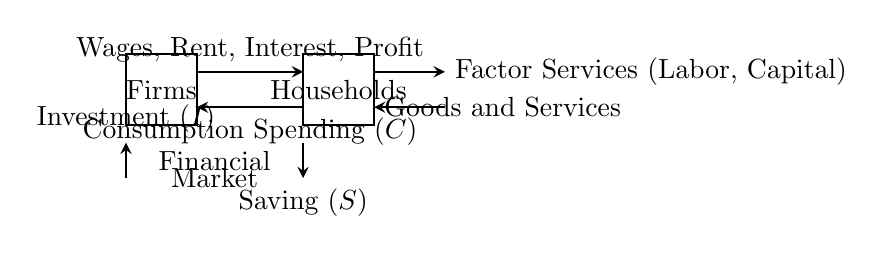
\begin{tikzpicture}[scale=0.45, thick, >=stealth]
    % Firms
    \draw (0,2) rectangle (2,4) node[midway] {Firms};
    % Households
    \draw (5,2) rectangle (7,4) node[midway] {Households};
    % Flows
    \draw[->] (2,3.5) -- (5,3.5) node[midway, above] {Wages, Rent, Interest, Profit};
    \draw[->] (5,2.5) -- (2,2.5) node[midway, below] {Consumption Spending ($C$)};
    \draw[->] (7,3.5) -- (9,3.5) node[right] {Factor Services (Labor, Capital)};
    \draw[->] (9,2.5) -- (7,2.5) node[right] {Goods and Services};
    \draw[->] (5,1.5) -- (5,0.5) node[below] {Saving ($S$)};
    \draw[->] (0,0.5) -- (0,1.5) node[above] {Investment ($I$)};
    \node at (2.5,1) {Financial};
    \node at (2.5,0.5) {Market};
\end{tikzpicture}
\end{center}
\textit{Inner loop: Real flows (factors, goods). Outer loop: Money flows (income, spending). Leakage: Saving. Injection: Investment. In equilibrium: $S = I$.}

\subsection*{Keynesian Cross: Equilibrium Output}
\begin{center}
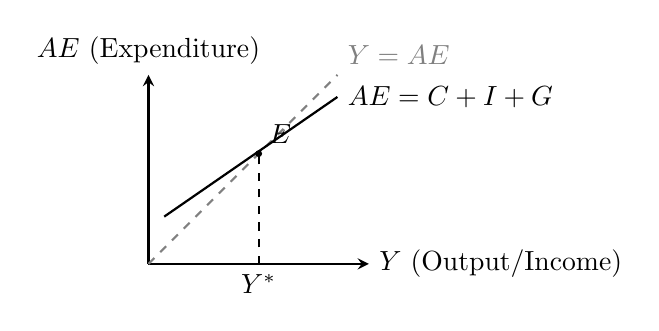
\begin{tikzpicture}[scale=0.4, thick, >=stealth]
    \draw[->] (0,0) -- (7,0) node[right] {$Y$ (Output/Income)};
    \draw[->] (0,0) -- (0,6) node[above] {$AE$ (Expenditure)};
    % 45-degree line
    \draw[thick, dashed, gray] (0,0) -- (6,6) node[above right] {$Y=AE$};
    % AE curve
    \draw[thick] (0.5,1.5) -- (6,5.3) node[right] {$AE = C + I + G$};
    % Equilibrium
    \filldraw (3.5,3.5) circle (2pt) node[above right] {$E$};
    \draw[dashed] (3.5,0) node[below] {$Y^*$} -- (3.5,3.5);
\end{tikzpicture}
\end{center}
\textit{Equilibrium where $AE$ line intersects the 45-degree line ($Y=AE$). If $Y < Y^*$, inventories fall unexpectedly, firms increase production. The multiplier amplifies changes in autonomous spending.}

\subsection*{Phillips Curve (Short-Run vs. Long-Run)}
\begin{center}
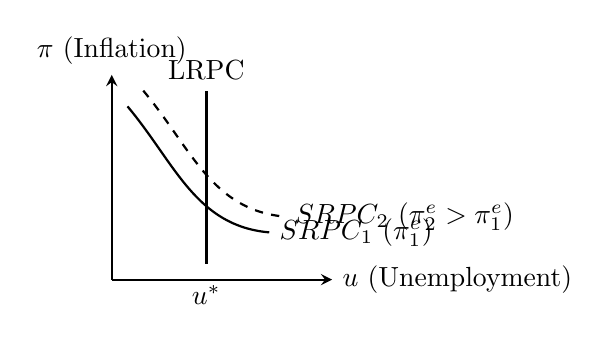
\begin{tikzpicture}[scale=0.4, thick, >=stealth]
    \draw[->] (0,0) -- (7,0) node[right] {$u$ (Unemployment)};
    \draw[->] (0,0) -- (0,6.5) node[above] {$\pi$ (Inflation)};
    % LRPC (vertical)
    \draw[very thick] (3,0.5) -- (3,6) node[above] {LRPC};
    \node at (3,-0.5) {$u^*$};
    % SRPC curves
    \draw[thick] (0.5,5.5) to[out=310, in=175] (5,1.5) node[right] {$SRPC_1$ ($\pi^e_1$)};
    \draw[thick, dashed] (1,6) to[out=310, in=175] (5.5,2) node[right] {$SRPC_2$ ($\pi^e_2 > \pi^e_1$)};
\end{tikzpicture}
\end{center}
\textit{Short-run Phillips Curve (SRPC) slopes down: lower unemployment temporarily achievable with higher inflation. Long-run Phillips Curve (LRPC) is vertical at the Natural Rate of Unemployment ($u^*$): no long-run trade-off.}

% ============================================================================
% PART 5: FISCAL AND MONETARY POLICY
% ============================================================================
\section*{5. Macroeconomic Policy}

\subsection*{Fiscal Policy}
Conducted by the \textbf{government} (Treasury/Finance Ministry). Uses \textbf{government spending ($G$)} and \textbf{taxation ($T$)} to influence aggregate demand.
\begin{itemize}[leftmargin=*,nosep]
    \item \textbf{Expansionary:} Increase $G$ or decrease $T$ $\to$ boosts AD (shifts AE up/IS right). Used during recession. Financed by borrowing (deficit spending).
    \item \textbf{Contractionary:} Decrease $G$ or increase $T$ $\to$ reduces AD. Used to cool overheating economy, combat inflation.
    \item \textbf{Automatic Stabilizers:} Built-in features that automatically adjust: progressive taxes (revenues fall in recession), unemployment benefits (spending rises). No new legislation required.
    \item \textbf{Limitations:} \textbf{Crowding out} -- government borrowing raises interest rates, reducing private investment. \textbf{Time lags} -- recognition, implementation, and impact lags. \textbf{Ricardian equivalence} -- consumers save tax cuts anticipating future tax hikes, neutralizing fiscal stimulus.
\end{itemize}

\subsection*{Monetary Policy}
Conducted by the \textbf{Central Bank} (e.g., Federal Reserve, ECB). Manages \textbf{money supply} and \textbf{interest rates} to achieve price stability, full employment, and economic growth.
\begin{itemize}[leftmargin=*,nosep]
    \item \textbf{Tools:}
    \begin{enumerate}[nosep]
        \item \textbf{Policy Interest Rate (e.g., Federal Funds Rate):} Lower rate $\to$ cheaper borrowing $\to$ stimulates investment and consumption $\to$ AD shifts right. Higher rate to cool economy.
        \item \textbf{Open Market Operations (OMOs):} Buying government bonds injects money into banking system (expansionary). Selling bonds withdraws money (contractionary).
        \item \textbf{Reserve Requirements:} Lower required reserve ratio allows banks to lend more. Rarely changed.
        \item \textbf{Quantitative Easing (QE):} Central bank purchases long-term securities to lower long-term rates when short-term rates near zero. Used extensively post-2008 and COVID-19.
    \end{enumerate}
    \item \textbf{Transmission Mechanism:} Policy rate $\downarrow$ $\to$ market rates $\downarrow$ $\to$ borrowing $\uparrow$ $\to$ $C$ and $I$ $\uparrow$ $\to$ AD $\uparrow$ $\to$ Output $\uparrow$, Unemployment $\downarrow$.
    \item \textbf{Inflation Targeting:} Many central banks target ~2\% inflation. If inflation exceeds target, they raise rates.
    \item \textbf{Limitations:} \textbf{Liquidity trap} -- interest rates are near zero, monetary policy ineffective (Keynesian). \textbf{Long and variable lags} (Milton Friedman).
\end{itemize}

\subsection*{Policy Mix}
Fiscal and monetary policies can work together or at cross-purposes. Example: 2008--2009 Global Financial Crisis saw coordinated expansionary fiscal (stimulus packages) and monetary (near-zero rates, QE) policy globally.

\columnbreak

% ============================================================================
% PART 6: EXTENSIVE CASE STUDIES
% ============================================================================
\section*{6. Comprehensive Case Studies}

\subsection*{Case Study 1: The Great Recession (2008--2009) and the Global Policy Response}

\textbf{Background:} The subprime mortgage crisis in the US triggered a global financial meltdown. Banks collapsed (Lehman Brothers, Sept 2008), credit markets froze, and aggregate demand plummeted. The world entered the deepest recession since the 1930s.

\textbf{Macroeconomic Impact:}
\begin{itemize}[leftmargin=*,nosep]
    \item \textbf{US GDP:} Fell by 4.3\% from peak (Dec 2007) to trough (June 2009).
    \item \textbf{Unemployment:} US unemployment rate doubled from 5.0\% (Dec 2007) to 10.0\% (Oct 2009). Cyclical unemployment surged.
    \item \textbf{Inflation:} Plummeted; fears of deflation emerged (CPI briefly negative in 2009).
    \item \textbf{Global Spillover:} World trade collapsed by over 20\%. Export-dependent economies (Germany, Japan, China) severely hit. GDP contracted globally in 2009 -- the first global GDP decline since WWII.
\end{itemize}

\textbf{Policy Response: Unprecedented Monetary and Fiscal Expansion.}

\textit{1. Monetary Policy (Federal Reserve):}
\begin{itemize}[leftmargin=*,nosep]
    \item \textbf{Interest Rate Cuts:} Fed cut Federal Funds Rate from 5.25\% (Aug 2007) to 0--0.25\% (Dec 2008). Effectively hit the \textbf{zero lower bound}.
    \item \textbf{Quantitative Easing (QE1):} With rates at zero, the Fed launched massive asset purchases. Between 2008 and 2014, the Fed's balance sheet expanded from \$900 billion to over \$4.5 trillion. Purchased mortgage-backed securities (MBS) and Treasury bonds to lower long-term rates, support housing market, and inject liquidity.
    \item \textbf{Credit Facilities:} Created special lending facilities to unfreeze commercial paper, money market, and corporate bond markets.
    \item \textbf{Effectiveness:} Prevented a complete financial meltdown. Lowered long-term mortgage rates to historical lows, supporting a housing recovery. Critics argued QE contributed to asset price bubbles and wealth inequality (wealth effect benefited asset holders).
\end{itemize}

\textit{2. Fiscal Policy (US Government):}
\begin{itemize}[leftmargin=*,nosep]
    \item \textbf{Economic Stimulus Act (2008):} \$152 billion in tax rebates. Modest impact.
    \item \textbf{American Recovery and Reinvestment Act (ARRA, 2009):} \$787 billion (later revised to \$831 billion). Largest fiscal stimulus in US history at the time. Comprised:
    \begin{itemize}[nosep]
        \item \textbf{Tax cuts (\$288B):} Personal and business tax reductions.
        \item \textbf{Spending (\$499B):} Infrastructure, education, healthcare, renewable energy, aid to states.
    \end{itemize}
    \item \textbf{Automatic Stabilizers:} Unemployment insurance extensions, food stamps (SNAP) expanded automatically, providing significant income support without new legislation.
\end{itemize}

\textbf{Analysis Using Keynesian Cross Multiplier:}
Assume MPC ($b$) = 0.6. Multiplier $k = 1/(1-0.6) = 2.5$. A \$800B fiscal stimulus would theoretically boost GDP by up to \$2,000B (if no crowding out). In reality, the multiplier was likely smaller (0.5--1.5) due to:
\begin{itemize}[nosep]
    \item \textbf{Crowding out:} Some private investment displaced (though limited at zero rates).
    \item \textbf{Imports:} Part of spending leaked abroad (open-economy multiplier smaller).
    \item \textbf{Ricardian effects:} Households saved part of tax cuts.
    \item \textbf{Uncertainty:} Deep uncertainty reduced MPC (precautionary saving rose).
\end{itemize}
Nevertheless, most economists (CBO, IMF estimates) conclude the ARRA saved/created 2--3 million jobs and prevented a much deeper recession.

\textbf{NPV of Bailouts vs. Fiscal Stimulus:}
TARP (Troubled Asset Relief Program, 2008) to bail out banks: \$700B authorized. Surprisingly, the government \textbf{earned a positive return} on bank bailouts (\~ +{\$}20B) because banks repaid with interest. CBA showed fiscal cost was minimal. NPV of auto bailout (GM, Chrysler) was arguably positive due to saved jobs and supply chains versus long-run cost.

\textbf{Global Dimensions:}
\begin{itemize}[leftmargin=*,nosep]
    \item \textbf{China:} Massive \$586B fiscal stimulus (2008--2010), mostly infrastructure investment. GDP growth remained > 8\%, preventing global depression.
    \item \textbf{Europe:} ECB cut rates but was slower. Sovereign debt crisis (Greece, 2010) forced \textbf{austerity} (contractionary fiscal policy) in the periphery, prolonging recession. Contrast with US/China expansion.
\end{itemize}

\textbf{Economic Lessons:}
\begin{enumerate}[leftmargin=*,nosep]
    \item \textbf{Zero lower bound} constrains conventional monetary policy; unconventional tools (QE) are essential but have side effects.
    \item \textbf{Fiscal policy} is a critical complement when monetary policy is exhausted.
    \item \textbf{Coordination} matters: simultaneous global fiscal expansion was more effective than any country acting alone (positive spillovers via trade).
    \item \textbf{Political economy:} Austerity during a liquidity trap is self-defeating; it deepens recession and increases debt/GDP ratio (as GDP denominator shrinks).
    \item \textbf{Investment decisions} during crisis must consider extreme uncertainty: NPV and IRR calculations fail if future cash flows are radically uncertain. Firms delayed investment despite low rates (``wait and see'' option value).
\end{enumerate}

\subsection*{Case Study 2: The Post-COVID Inflation Surge (2021--2023) and the Return of Monetary Tightening}

\textbf{Background:} After COVID-19 hit in 2020, governments and central banks unleashed an even larger stimulus than 2008. As the economy reopened, demand surged but supply chains were broken, leading to the highest inflation in 40 years.

\textbf{The Shock and Policy:}
\begin{itemize}[leftmargin=*,nosep]
    \item \textbf{Fiscal Stimulus:} US: \$2.2T CARES Act (2020), \$900B relief (Dec 2020), \$1.9T American Rescue Plan (March 2021). Total \~ \$5T, \~ 25\% of GDP.
    \item \textbf{Monetary Easing:} Fed cut rates to 0\%, resumed massive QE (\$120B/month purchases). ECB, BoJ, BoE similar.
    \item \textbf{Direct Transfers:} Unprecedented direct checks to households (\$1,200 + \$600 + \$1,400 per adult) boosted \textbf{disposable income} even as GDP fell temporarily. \textbf{Personal saving rate} spiked to 33\% (April 2020).
\end{itemize}

\textbf{Inflationary Mechanism:}
As vaccines rolled out (2021), pent-up demand exploded. But supply couldn't respond:
\begin{itemize}[leftmargin=*,nosep]
    \item \textbf{Goods demand surge:} Consumers shifted from services (travel, dining) to goods (electronics, furniture, home improvement).
    \item \textbf{Supply chain bottlenecks:} Port congestion (LA/Long Beach), semiconductor shortage (Case Study in Topic 2), labor shortages (``Great Resignation''), shipping container costs up 500\%.
    \item \textbf{Energy price spike:} Russia-Ukraine war (Feb 2022) sent oil and natural gas prices soaring (cost-push shock).
    \item \textbf{Inflation:} US CPI inflation hit 9.1\% (June 2022), UK > 11\%, Eurozone > 10\%. Far above 2\% targets.
\end{itemize}

\textbf{Monetary Policy Reversal (2022--2023):}
Central banks pivoted aggressively from easing to tightening:
\begin{itemize}[leftmargin=*,nosep]
    \item \textbf{Fed:} Raised rates from 0.25\% to 5.50\% (March 2022--July 2023) -- fastest tightening in 40 years. Began Quantitative Tightening (QT) -- shrinking balance sheet.
    \item \textbf{Transmission:} Mortgage rates jumped from 3\% to 7\%+. Housing market cooled. Business investment slowed.
    \item \textbf{Goal:} Reduce aggregate demand to bring it in line with constrained supply, cooling inflation without causing deep recession (``soft landing'').
\end{itemize}

\textbf{Evaluation of Policy -- The Soft Landing Debate:}
By mid-2024, inflation had fallen to \~ 3\% without a large rise in unemployment (remained below 4\%). This ``immaculate disinflation'' surprised many economists. Possible reasons:
\begin{enumerate}[leftmargin=*,nosep]
    \item \textbf{Supply recovery:} Bottlenecks eased; labor force participation recovered.
    \item \textbf{Well-anchored expectations:} Despite high inflation, long-term inflation expectations remained near 2\%, so \textbf{Phillips Curve} remained flat (inflation fell without requiring large unemployment increase).
    \item \textbf{Lags:} Full effect of rate hikes may still be in pipeline; recession risk not eliminated.
    \item \textbf{Fiscal contraction:} Pandemic stimulus expired, acting as automatic fiscal tightening.
\end{enumerate}

\textbf{Investment Decisions in High-Inflation Environment:}
Firms evaluating projects in 2022--2023 faced:
\begin{itemize}[leftmargin=*,nosep]
    \item \textbf{Higher discount rate ($r$):} As central bank rates rose, cost of capital ($r$) increased, reducing \textbf{NPV} of long-term projects. Green energy capital-intensive projects (wind, solar) were particularly sensitive to higher rates.
    \item \textbf{Inflation in cash flows:} Nominal revenues rose with inflation, but real costs uncertain. Distinction between real and nominal NPV became critical.
    \item \textbf{Uncertainty:} High inflation volatility made forecasting future cash flows more difficult, increasing the ``option value of waiting'' and delaying irreversible investment.
    \item \textbf{Payback period became more popular:} In uncertain times, firms favored projects with faster payback to reduce risk exposure.
\end{itemize}
\textit{Example NPV Shift:} A \$100M renewable project with \$10M annual real cash flow for 20 years. At $r = 0.04$ (real): $NPV \approx -\$100M + \$135.9M = +\$35.9M$ (Accept). At $r = 0.08$ (real, after rate hikes): $NPV = -\$100M + \$98.2M = -\$1.8M$ (Reject). Monetary tightening directly kills marginal projects.

\textbf{Economic Lessons:}
\begin{enumerate}[leftmargin=*,nosep]
    \item \textbf{Inflation} can emerge from a combination of demand-pull (massive fiscal stimulus) and cost-push (supply chain, energy) shocks.
    \item \textbf{Monetary policy} operates with lags; central banks risk over-tightening if they don't account for them.
    \item \textbf{Real vs. Nominal} distinctions are crucial for investment evaluation under changing inflation.
    \item \textbf{Fiscal-monetary interaction:} Generous fiscal transfers during supply constraints contributed to inflation, creating a policy dilemma: support citizens vs. control inflation.
    \item \textbf{The Phillips curve} is not stable; it depends on expectations, supply conditions, and credibility of central banks.
\end{enumerate}

% ============================================================================
% PART 7: EXAM QUESTIONS
% ============================================================================
\section*{7. Exam Questions \& Model Answers}

\subsection*{Question 1: National Income Calculation}
\textbf{Given the following data for a closed economy (in \$ billions): $C = 200 + 0.75Y_d$, $I = 300$, $G = 400$, $T = 200$ (lump-sum tax).}
\textbf{(a) Find equilibrium GDP.}
\textbf{(b) Calculate the government spending multiplier.}
\textbf{(c) If potential GDP is 2,800, what change in $G$ is needed to close the output gap?}
\textbf{(d) If the government simultaneously increases $G$ by 50 and $T$ by 50, what happens to equilibrium GDP? (Balanced Budget Multiplier)}

\vspace{0.05cm}
\textbf{Solution:}
\vspace{0.05cm}
\textbf{(a)} $Y_d = Y - T = Y - 200$. $AE = 200 + 0.75(Y-200) + 300 + 400 = 200 + 0.75Y - 150 + 700 = 750 + 0.75Y$. Set $Y = AE$: $Y = 750 + 0.75Y \Rightarrow 0.25Y = 750 \Rightarrow \mathbf{Y^* = 3000}$.

\textbf{(b)} Multiplier $k = 1/(1-0.75) = 1/0.25 = \mathbf{4}$.

\textbf{(c)} Output gap = $2800 - 3000 = -200$ (recessionary gap, though note 3000 > 2800, i.e., economy is above potential, i.e., inflationary gap). If potential = 2800, and current = 3000, gap = +200. To close, need $\Delta Y = -200$. $\Delta G = \Delta Y / k = -200 / 4 = \mathbf{-50}$. Reduce $G$ by 50.

\textbf{(d)} Balanced budget multiplier: $\Delta G = \Delta T = 50$. Effect: $\Delta Y = k \cdot \Delta G + k_T \cdot \Delta T$, where $k_T = -b/(1-b) = -0.75/0.25 = -3$. $\Delta Y = 4(50) + (-3)(50) = 200 - 150 = +50$.
The \textbf{Balanced Budget Multiplier = 1}: equal increase in $G$ and $T$ raises Y exactly by the amount of the increase. (Here, $1/(1-b) + (-b/(1-b)) = (1-b)/(1-b) = 1$).

\vspace{0.2cm}

\subsection*{Question 2: Real vs. Nominal GDP and Deflator}
\textbf{An economy produces only apples and oranges. Data: Base Year 2020.}

\begin{center}
\begin{tabular}{@{}l|cc|cc@{}}
\toprule
& \multicolumn{2}{c|}{\textbf{2020}} & \multicolumn{2}{c}{\textbf{2023}} \\
& Qty & Price & Qty & Price \\
\midrule
Apples & 100 & \$2 & 120 & \$3 \\
Oranges & 50 & \$4 & 60 & \$5 \\
\bottomrule
\end{tabular}
\end{center}

\textbf{(a) Calculate Nominal GDP in 2020 and 2023.}
\textbf{(b) Calculate Real GDP in 2023 at 2020 prices.}
\textbf{(c) Calculate the GDP Deflator for 2023.}
\textbf{(d) What is the growth rate of real GDP from 2020 to 2023?}

\vspace{0.05cm}
\textbf{Solution:}
\vspace{0.05cm}
\textbf{(a)} Nominal 2020 = $100(2) + 50(4) = 200 + 200 = \mathbf{400}$. Nominal 2023 = $120(3) + 60(5) = 360 + 300 = \mathbf{660}$.

\textbf{(b)} Real 2023 (at 2020 prices) = $120(2) + 60(4) = 240 + 240 = \mathbf{480}$.

\textbf{(c)} Deflator 2023 = $(660/480) \times 100 = \mathbf{137.5}$.

\textbf{(d)} Real GDP 2020 = Nominal 2020 = 400 (base year). Real growth = $(480 - 400) / 400 \times 100 = \mathbf{20\%}$. (Nominal growth was 65\%, but much was inflation.)

\vspace{0.2cm}

\subsection*{Question 3: Investment Appraisal}
\textbf{A project requires initial investment of \$500,000. Expected net cash flows: Year 1: \$150,000; Year 2: \$200,000; Year 3: \$250,000; Year 4: \$100,000. Discount rate = 10\%.}
\textbf{(a) Calculate NPV. Should the project be accepted?}
\textbf{(b) Calculate the payback period.}
\textbf{(c) If the discount rate rises to 15\%, recalculate NPV. Explain the change.}

\vspace{0.05cm}
\textbf{Solution:}
\vspace{0.05cm}
\textbf{(a)} 
$NPV = -500,000 + \frac{150,000}{1.1} + \frac{200,000}{1.1^2} + \frac{250,000}{1.1^3} + \frac{100,000}{1.1^4}$
$= -500,000 + 136,363.6 + 165,289.3 + 187,828.7 + 68,301.3$
$= -500,000 + 557,782.9 = \mathbf{+\$57,783}$. Since $NPV > 0$, \textbf{accept}.

\textbf{(b)} Cumulative cash flows: Y1: \$150,000; Y2: \$350,000; Y3: \$600,000. Initial investment \$500,000 recovered between Y2 and Y3. Fraction of Y3 needed: $(500,000 - 350,000) / 250,000 = 0.6$. Payback = \textbf{2.6 years}.

\textbf{(c)} At 15\%:
$NPV = -500,000 + 130,434.8 + 151,228.7 + 164,379.1 + 57,175.3 = -500,000 + 503,217.9 = +\$3,218$ (still positive, just barely). Higher discount rate reduces PV of distant cash flows, reducing NPV. If $r$ rises enough, NPV turns negative $\to$ reject project.

\vspace{0.2cm}

\subsection*{Question 4: Policy Analysis}
\textbf{Explain, using AD-AS or IS-LM logic, why a central bank would raise interest rates in response to high inflation. What are the risks?}

\vspace{0.05cm}
\textbf{Answer:} High inflation indicates aggregate demand exceeds aggregate supply (or supply has contracted). Raising the policy interest rate makes borrowing more expensive, reducing consumption (durables, housing) and business investment. This shifts the AD curve leftward (or shifts LM up/left), reducing output and thus reducing inflationary pressure. The \textbf{risk} is that monetary policy operates with ``long and variable lags'' (Friedman). If the central bank tightens too aggressively or late, it may: (1) overshoot and cause a recession (AD falls too much below potential), leading to unemployment; (2) fail to anchor expectations, causing a wage-price spiral; (3) trigger a financial crisis if highly leveraged sectors (real estate, banks) cannot handle higher rates; (4) exacerbate fiscal sustainability issues by raising government borrowing costs. A ``soft landing'' (reducing inflation without recession) is the goal, but historically difficult.

\end{multicols}

% ============================================================================
% SUMMARY TABLE
% ============================================================================
\vspace{0.3cm}
\begin{center}
\fbox{\begin{minipage}{0.9\textwidth}
\footnotesize
\textbf{Summary Cheat Sheet: Macroeconomics}
\begin{center}
\begin{tabular}{@{}p{3cm}p{2.5cm}p{3.5cm}@{}}
\toprule
\textbf{Concept} & \textbf{Formula/Identity} & \textbf{Key Insight} \\
\midrule
GDP (Expenditure) & $Y = C + I + G + NX$ & Total spending = Total output \\
GNP & $GNP = GDP + NFIA$ & Based on residency, not geography \\
Real GDP & $\sum P_{\text{base}} Q_t$ & Removes inflation; measures true growth \\
GDP Deflator & $\frac{\text{Nominal GDP}}{\text{Real GDP}} \times 100$ & Broadest price index \\
Consumption Function & $C = a + bY_d$ & MPC ($b$) + MPS = 1 \\
Multiplier & $k = 1/(1-b)$ & Amplifies autonomous spending changes \\
Unemployment Rate & $u = \frac{U}{LF} \times 100$ & Excludes discouraged workers \\
Inflation Rate & $\pi = \frac{P_t - P_{t-1}}{P_{t-1}} \times 100$ & \% change in price level \\
NPV & $NPV = \sum CF_t / (1+r)^t$ & Accept if $NPV > 0$ \\
IRR & $NPV = 0 \to r^*$ & Accept if $IRR > \text{cost of capital}$ \\
Fiscal Policy & $G$ and $T$ & Government spending \& taxation \\
Monetary Policy & Interest rates, money supply & Central bank manages demand \\
\bottomrule
\end{tabular}
\end{center}

\vspace{0.1cm}
\textbf{Quick Policy Reference:}
\begin{itemize}[leftmargin=*,nosep]
    \item \textbf{Recession} $\to$ Expansionary: $\uparrow G$, $\downarrow T$, $\downarrow r$, QE.
    \item \textbf{Inflation} $\to$ Contractionary: $\downarrow G$, $\uparrow T$, $\uparrow r$, QT.
    \item \textbf{Liquidity Trap} $\to$ Monetary policy ineffective; rely on fiscal policy.
    \item \textbf{NPV Rule:} Positive NPV $\to$ Accept project; IRR > Hurdle Rate $\to$ Accept.
\end{itemize}
\end{minipage}}
\end{center}

\end{document}
\newpage

\end{document}